%*******10********20********30********40********50********60********70********80

% For all chapters, use the newdefined chap{} instead of chapter{}
% This will make the text at the top-left of the page be the same as the chapter

\chap{Θεωρητικό Υπόβαθρο και Σχετική Βιβλιογραφία} \label{c:complex}
%ΠΕΡΙΓΡΑΦΗ ΤΟΥ ΤΙ ΑΚΡΙΒΩΣ ΠΑΡΟΥΣΙΑΖΕΤΑΙ ΣΤΟ ΚΕΦΑΛΑΙΟ

Στο συγκεκριμένο κεφάλαιο γίνεται επεξήγηση των βασικών εννοιών και τεχνολογιών που αναφέρονται στην εργασία. Παρουσιάζονται οι έννοιες της Επαυξημένης Πραγματικότητας, του μοντέλου κάμερας pinhole, της ανίχνευσης δεικτών (markers) και το πεδίο της αναγνώρισης χειρονομιών σε εφαρμογές. Επιπλέον γίνεται ανασκόπηση των σχετικών επιστημονικών εργασιών και εφαρμογών, καθώς και των ανοικτών προκλήσεων στον ερευνητικό τομέα.



\section{Επαυξημένη Πραγματικότητα}
%ΟΡΙΣΜΟΣ+ΤΙ ΥΠΑΡΧΕΙ ΣΗΜΕΡΑ+ΔΙΑΦΟΡΑ ΑΠΟ VR+ OTI EXEI NA KANEI ME AR APO ERGASIES ALLON


%verykokou
Ο όρος επαυξημένη πραγματικότητα, διεθνώς γνωστή ως augmented reality (AR), αναφέρεται στην τεχνολογία που επιτρέπει την προσθήκη ψηφιακών πληροφοριών, που παράγονται από έναν υπολογιστή, στον πραγματικό κόσμο, μέσω κατάλληλων συσκευών. Πρόκειται για ένα ταχέως εξελισσόμενο ερευνητικό πεδίο, το οποίο στοχεύει στον εμπλουτισμό της αντίληψης της πραγματικότητας από το χρήστη.


Ιδανικά, τα αντικείμενα που συμπληρώνουν τον πραγματικό κόσμο παρουσιάζονται να συνυπάρχουν στον ίδιο χώρο με αυτόν. Ωστόσο, δεν αποτελούν μόνο οπτικές πληροφορίες. Η επαυξημένη πραγματικότητα, δυνητικά, μπορεί να βελτιώσει και τις πέντε αισθήσεις, και κυρίως – εκτός από την όραση – την ακοή και την αφή, αν και σήμερα η κυρίαρχη χρήση της είναι η προσθήκη οπτικών πληροφοριών στον πραγματικό κόσμο. 


Υπάρχουν διάφοροι ορισμοί της επαυξημένης πραγματικότητας, εκ των οποίων ευρέως αποδεκτός είναι ο ορισμός που έδωσε ο Ronald Azuma το 1997 \cite{azuma1997}. Σύμφωνα με αυτόν, η επαυξημένη πραγματικότητα είναι μία παραλλαγή της εικονικής πραγματικότητας (virtual reality), αλλά δε θα πρέπει να συγχέεται με την τελευταία, διότι συμπληρώνει τον πραγματικό κόσμο και δεν τον υποκαθιστά. 



Στόχος της εικονικής πραγματικότητας είναι η πλήρης «εμβύθιση» του χρήστη σε ένα περιβάλλον πλήρως ελεγχόμενο από υπολογιστή, το οποίο δεν του επιτρέπει να δει τον πραγματικό κόσμο γύρω του. Οι χρήστες εμβυθίζονται σε μία σκηνή που αν και αποτελείται εξ' ολοκλήρου από γραφικά, γίνται αντιληπτή σαν να ήταν πραγματική.  Για να δημιουργηθεί μια ρεαλιστική εικονική σκηνή, το επίπεδο των λεπτομερειών των γραφικών που συνιστούν τα αντικείμενα της εικονικής σκηνής πρέπει να είναι ιδιαίτερα υψηλό και η απεικόνιση πρέπει να πραγματοποιείται σε πραγματικό χρόνο. Ωστόσο όσο υψηλότερο είναι το επίπεδο των λεπτομερειών, τόσο μειώνεται η απόδοση ενός συστήματος προσπαθώντας να τα απεικονίσει. Ο συνθετικός αυτός κόσμος μπορεί να μιμείται τις ιδιότητες ενός πραγματικού κόσμου, είτε αυτός υπάρχει είτε όχι, ή και να διαφέρει σημαντικά από την πραγματικότητα, δημιουργώντας ένα φανταστικό κόσμο, στον οποίο οι φυσικοί νόμοι δεν ισχύουν πλέον [8]. 


Η επαυξημένη πραγματικότητα στοχεύει στην ενσωμάτωση συνθετικών πληροφοριών στο πραγματικό περιβάλλον – ή σε ένα βίντεο του πραγματικού περιβάλλοντος – με αποτέλεσμα αυτό να μην αποκρύπτεται εντελώς, αλλά αντίθετα να έχει κυρίαρχο ρόλο. Τα εικονικά αντικείμενα σε ένα περιβάλλον επαυξημένης πραγματικότητας, δεν είναι απαραίτητο να έχουν ένα υψηλό επίπεδο λεπτομερειών. Η ρεαλιστική ποιότητά τους περιορίζεται μόνο από τις παραμέτρους της εφαρμογής. 

Μία ακόμα διαφορά ανάμεσα σε συστήματα επαυξημένης και εικονικής πραγματικότητας βασίζεται στο ποσοστό του περιεχομένου της σκηνής που απεικονίζεται. Ένα σύστημα επαυξημένης πραγματικότητας, στο οποίο απεικονίζονται μόνο μερικά απλά εικονικά αντικείμενα σε μία σκηνή, απαιτεί λιγότερη ισχύ από ένα σύστημα εικονικής πραγματικότητας, στο οποίο πρέπει να απεικονίζεται ολόκληρη η σκηνή.


Επιπλέον, διαφορές ανάμεσα στα δύο συστήματα παρατηρούνται στο πρόβλημα του registration(γεωαναφορά). Αφού το registration ασχολείται με τη σωστή τοποθέτηση εικονικών αντικειμένων εντός ενός πραγματικού περιβάλλοντος, τα συστήματα εικονικής πραγματικότητας δεν επηρεάζονται, αφού έχουν να κάνουν μόνο με εικονικές σκηνές. Η θέση όλων των αντικειμένων σε μία σκηνή VR περιγράφεται με βάση ένα κοινό σύστημα συντεταγμένων. Αυτό σημαίνει ότι ένα σύστημα VR έχει πάντα σωστό registration χωρίς να πρέπει να σπαταλά υπολογιστικούς πόρους για την εύρεσή του. Όσον αφορά την απόδοση, το χαμηλό υπολογιστικό κόστος για απεικόνιση γραφικών χαμηλής ποιότητας αντισταθμίζεται από το υπολογιστικό κόστος που απαιτείται για το registration.

Τέλος, στα συστήματα VR, οι συσκευές απεικόνισης χρησιμοποιούνται για να ανιχνεύουν τη τη θέση του χρήστη μαζί με μία οθόνη που απεικονίζει την ψηφιακή σκηνή. Σε ένα σύστημα επαυξημένης πραγματικότητας, υπάρχουν πολλοί διαφορετκοί συνδυασμοί εξοπλισμοί για την ανίχνευση και την πληροφόρηση του χρήστη.
%---

Τα συστήματα επαυξημένης πραγματικότητας σύμφωνα με την καταπληκτική ερευνητική επισκόπηση του πεδίου από τους Azuma et al. (2001) έχουν τα ακόλουθα τρία χαρακτηριστικά \cite{azuma2001}:

\begin{itemize}
\item Συνδυάζουν το πραγματική με την εικονική πληροφορία
\item Επιτρέπουν την αλληλεπίδραση σε πραγματικό χρόνο
\item Λειτουργούν αναφορικά με τον πραγματικό τρισδιάστατο κόσμο
\end{itemize}  


Τα παραπάνω χαρακτηριστικά καθίστανται σημαντικά στην αξιολόγηση αν ένα σύστημα είναι σύστημα επαυξημένης πραγματικότητας ή όχι. Έτσι, για παράδειγμα, κάποιες ταινίες, μολονότι μπορεί να περιλαμβάνουν φωτορεαλιστικά εικονικά αντικείμενα τα οποία συνδυάζονται ομαλά με το τρισδιάστατο πραγματικό περιβάλλον, δεν είναι διαδραστικές σε πραγματικό χρόνο και επομένως δεν αποτελούν συστήματα επαυξημένης πραγματικότητας \cite{azuma1997}. Αντίθετα, η εισαγωγή των εικονικών δεδομένων οφείλεται σε προεπεξεργασία, η οποία αντιτίθεται με το δεύτερο χαρακτηριστικό των συστημάτων επαυξημένης πραγματικότητας.

%augmented virtuality continuum
Σύμφωνα με τους Paul Milgram et al. (1994), η επαυξημένη πραγματικότητα ανήκει στην τεχνολογία της μικτής πραγματικότητας (mixed reality) [8].

Στη δημοσίευσή τους, ορίζεται το «συνεχές πραγματικότητας - εικονικότητας» (reality - virtuality continuum), το οποίο μπορεί να χρησιμοποιηθεί για τη σύγκριση των διαφόρων μορφών της μεικτής πραγματικότητας με την τοποθέτησή τους σε ένα φάσμα, όπως φαίνεται στην Εικόνα 1-1. 

Στη μία άκρη του φάσματους βρίσκεται το πραγματικό περιβάλλον, που δεν περιέχει καμία εικονική πληροφορία. Ενώ μετακινούμαστε προς τα δεξιά, εντοπίζεται η επαυξημένη πραγματικότητα, όπου τα τεχνητά αντικείμενα προστίθενται στον φυσικό κόσμο. Αμέσως πιο δεξιά, εντοπίζεται η επαυξημένη εικονικότητα, όπου τα αντικείμενα του φυσικού κόσμου(όπως μία ζωντανή απεικόνιση μίας απομακρυσμένης προβολής) προστίθενται σε ένα πλήρως εικονικό περιβάλλον "εμβύθισης". Φτάνοντας στο δεξί άκρος του φάσματος, παρατηρείται ένα πλήρως συνθετικό περιβάλλον, στο οποίο δεν υπάρχει καμία πληροφορία από τον φυσικό κόσμο.Κάθε είδος 3D περιβάλλοντος μπορεί να τοποθετηθεί κατά μήκος του φάσματος και μπορεί να χρησιμοποιηθεί για την εύκολη σύγκριση των χαρακτηριστικών του.

Επομένως στο περιβάλλον μεικτής πραγματικότητας, αντικείμενα του πραγματικού και του εικονικού κόσμου – δηλαδή οτιδήποτε μεταξύ των άκρων του συνεχούς – παρουσιάζονται μαζί σε μία συσκευή θέασης. Η μεικτή πραγματικότητα περιλαμβάνει τόσο την επαυξημένη πραγματικότητα, όσο και την επαυξημένη εικονικότητα (augmented virtuality). Ενώ στην πρώτη, το περιβάλλον που παρατηρείται είναι κυρίως αληθινό και έχουν προστεθεί βελτιώσεις που παράγονται από υπολογιστή, στην επαυξημένη εικονικότητα το παρατηρούμενο περιβάλλον είναι κυρίως εικονικό και επαυξάνεται με τη χρήση πραγματικών δεδομένων.

%ADD IMAGE OF CONTINUUM

Αυτός ο ορισμός δεν περιορίζει την επαυξημένη πραγματικότητα στη χρήση μόνο συσκευών απεικόνισης που τοποθετούνται στο κεφάλι του χρήστη(HMDs), επιτρέποντας τη χρήση προβολέων και φορητών συσκευών απεικόνισης, αλλά απκλείοντας μη διαδραστικά μέσα όπως οι ταινίες και τα τηλεοπτικά δρώμενα. 

Για να υπερθέσουμε τρισδιάστατα εικονικά μοντέλα σε αυτ΄που βλέπουν οι χρήστες, ένα σύστημα ΑR πρέπει να συνδυάζει τις πληροφορίες που παράγονται από έναν υπολογιστή με αισθητήρες που μπορούν να μετρήσουν τη θέση και τον προσανατολισμό του χρήστη. 

Καθώς ο χρήστης κινείται στο φυσικό κόσμο, η απεικόνιση των πληροφοριών ανανεώνεται σε πραγματικό χρόνο από τον υπολογιστή. Η ακρίβεια της τοποθέτησης των εικονικών αντικειμένων πάνω στο φυσικό κόσμο επηρεάζει τον ρεαλισμό της εμπειρίας του χρήστη.


%-----------


%AR=Combination of Computer Graphics & COmputer Vision
Ουσιαστικά η επαυξημένη πραγματικότητα αποτελεί συνδυασμό του κλάδου των Γραφικών Υπολογιστών και της Όρασης Υπολογιστών. Ο συνδυασμός αλγορίθμων και μεθόδων των δύο αυτών συγγενών επιστημών είναι το κλειδί για την επίτευξη σημαντικών αποτελεσμάτων σε εφαρμογές που επεξεργάζονται εικόνες ή βίντεο, εξάγουν πληροφορίες από μία σκηνή και επαυξάνουν τη σκηνή με γραφικά.

Για να μπορέσει ο υπολογιστής να δημιουργήσει συναφείς πληροφορίες, πρέπει πρώτα να κατανοήσει κάποιες παραμέτρους. Οι παράμετροι αυτοί έχουν να κάνουν με πληροφορίες σχετικά με το περιβάλλον στο οποίο βρίσκεται ο χρήστης, καθώς και με τη θέση και τον προσανατολισμό του μέσα στο περιβάλλον αυτό. Με βάση αυτές τις πληροφορίες, ο υπολογιστής μπορεί να τοποθετήσει τις επαυξημένες πληροφορίες σωστά σε σχέση με τoν περιβάλλοντα χώρο. Αυτή η εναρμόνιση των εικονικών αντικειμένων με αντικείμενα της πραγματικής σκηνή είναι γνωστή με τον όρο registration. 

Η ανάπτυξη των τεχνικών της όρασης υπολογιστών συντελεί στην καλύτερη αναγνώριση της σκηνής και την εξαγωγή χαρακτηριστικών που βοηθούν στη γνώση της ακριβούς τοποθεσίας στην οποία πρέπει να τοποθετηθούν τα εικονικά αντικείμενα. Ορισμένες ερευνητικές μέθοδοι που αναπτύχθηκαν στο πεδίο της όρασης υπολογιστών εφαρμόζονται και σε συστήματα επαυξημένης πραγματικότητας. Μερικές από αυτές είναι ο εντοπισμός και η ανίχνευση markers και χαρακτηριστικών μία σκηνής, η ανίχνευση και ο εντοπισμός κίνησης, η ανάλυση εικόνας, η αναγνώριση χειρονομιών και η κατασκευή περιβαλλόντων που περιέχουν έναν αριθμό από διαφορετικούς αισθητήρες.


Από την άλλη πλευρά, τα γραφικά συντελούν στην επαύξηση της πραγματικότητας με τη φωτορεαλιστική απεικόνιση τρισδιάστατων μοντέλων σε πραγματικό χρόνο, και τις διαδραστικές κινήσεις τους (animations)

%-------------------------------------------------


Ένα τυπικό σύστημα επαυξημένης πραγματικότητας μπορεί να διαιρεθεί σε 2 κύριες εργασίες: το tracking και το registration.
Πρέπει δηλαδή να ανιχνευθεί ένα γνωστό πρότυπο που είναι αποθηκευμένο στη μνήμη ενός υπολογιστή(marker tracking) \cite{krevelen2010} και έπειτα να προστεθεί ένα εικονικό αντικείμενο στη σκηνή σωστά πάνω σε αυτό το πρότυπο.



\subsection{Ιστορική Αναδρομή}
%ΣΥΝΤΟΜΗ ΙΣΤΟΡΙΚΗ ΑΝΑΔΡΟΜΗ ΑΠΟ ΑΛΛΕΣ ΕΡΓΑΣΙΕΣ

Η τεχνολογίας της επαυξημένης πραγματικότητας υπαινίσσεται για πρώτη φορά το 1901, μέσα από το μυθιστόρημά του Frank Baum με τίτλο «The Master Key», όπου περιγράφεται ένα ζευγάρι ειδικών γυαλιών, το οποίο υπερθέτει στο μέτωπο του κάθε ανθρώπου, που βρίσκεται στο οπτικό πεδίο εκείνου που φοράει τα γυαλιά, ένα γράμμα το οποίο περιγράφει το χαρακτήρα του. [1] [9].


Τα πρώτα πρωτότυπα επαυξημένης πραγματικότητας(Fig. 3), δημιουργήθηκαν από τον πρωτοπόρο στην επιστήμη των γραφικών υπολογιστών Ivan Sutherland και τους φοιτητές του στα πανεπιστήμια του Harvard και της Utah, την δεκαετία του 1960 [151]. Συγκεκριμένα κατασκεύασαν μία τρισδιάστατη συσκευή απεικόνισης που τοποθετείται στο κεφάλι του χρήστη, ενώ παράλληλα κρέμεται από το ταβάνι, με σκοπό να επαυξήσει την σκηνή με τρισδιάστατες πληροφορίες, παρουσιάζοντας στο χρήστη μία προοπτική εικόνα, η οποία αλλάζει καθώς αυτός κουνά το κεφάλι του ή κινείται σε μία περιορισμένη περιοχή. Λόγω των ειδικών κατόπτρων στα πρίσματα μέσω των οποίων ο χρήστης κοιτάζει, μπορεί να βλέπει ταυτόχρονα τόσο τις εικόνες αυτές όσο και αντικείμενα από τον πραγματικό χώρο. Οι εικόνες που παρουσιάζονται στο χρήστη είναι εικόνες διάφανων τρισδιάστατων αντικειμένων, τα οποία αποτελούνται μόνο από τις κύριες ακμές τους και όχι συμπαγών τρισδιάστατων αντικειμένων, λόγω των τεχνικών περιορισμών της εποχής. Το συγκεκριμένο σύστημα θεωρείται, ωστόσο, το πρώτο σύστημα επαυξημένης πραγματικότητας και είναι πραγματικά καινοτόμο για την εποχή. \cite{sutherland1968head}


 

Το 1975 ο Myron Krueger δημιουργεί ένα εργαστήριο τεχνητής πραγματικότητας με το όνομα "Videoplace" στο Πανεπιστήμιο του Κονέκτικατ στις Ηνωμένες Πολιτείες, το οποίο αποτελείται από δύο ή περισσότερα δωμάτια που μπορεί να απέχουν οποιαδήποτε απόσταση μεταξύ τους, μία οθόνη προβολής σε κάθε δωμάτιο και ειδικό hardware, έτσι ώστε οι χρήστες να βλέπουν την εικόνα τους ως μία λευκή σιλουέτα στην οθόνη προβολής να κάνει τις ίδιες κινήσεις με αυτούς. Ταυτόχρονα, δίνεται η δυνατότητα αλληλεπίδρασης με γραφικά αντικείμενα της οθόνης, όπως κείμενο. Επίσης, η εικόνα κάθε χρήστη μπορεί να χρωματιστεί, να σμικρυνθεί ή να περιστραφεί, ενώ γενικά προσφέρονται πολλοί τρόποι αλληλεπίδρασης, όπως η ζωγραφική με τα δάκτυλα [12], [13], [14]. 


Στις αρχές της δεκαετίες του 1990, και συγκεκριμένα το 1992, επινοείται ο όρος "επαυξημένη πραγματικότητα" από δύο επιστήμονες που εργάζονταν στη Boeing, τους Caudell and Mizell [42], οι οποίοι ανέπτυξαν ένα πειραματικό σύστημα επαυξημένης πραγματικότητας για να βοηθήσουν τους εργάτες να συναρμολογήσουν τις πολύπλοκες δέσμες καλωδίων των αεροσκφών[21]. Η εικόνα Figure 1 παρουσιάζει το HMD που αναπτύχθηκε.


Το ίδιο έτος, οι Steven Feiner, Blair MacIntyre και Doree Seligmann παρουσιάζουν το πρώτο κύριο άρθρο πάνω σε ένα πρωτότυπο σύστημα επαυξημένης πραγματικότητας (βλ. Εικόνα 1-4). Tο σύστημα αυτό, με την ονομασία KARMA («Knowledge-based Augmented Reality Maintenance Assistance»), χρησιμοποιεί ένα σύστημα HMD για την υποβοήθηση του τελικού χρήστη κατά τη συντήρηση ενός εκτυπωτή laser \cite{feiner1993knowledge}.



Το 1994, όπως αναφέραμε και σε προηγούμενη ενότητα, ο Paul Milgram παρουσίασε το συνεχές εικονικότητας-πραγματικότητας\cite{milgram1994taxonomy}, το οποίο αποκαλείται και συνεχές επαυξημένης πραγματικότητας. Την ίδια χρονιά, η επαυξημένη πραγματικότητα εισάγεται στο χώρο της τέχνης και της διασκέδασης, αφού δημιουργείται η πρώτη θεατρική παραγωγή επαυξημένης πραγματικότητας με την ονομασία «Dancing in Cyberspace», στην οποία χορευτές και ακροβάτες αλληλεπιδρούν με εικονικά αντικείμενα σε πραγματικό χρόνο, τα οποία προβάλλονται στη σκηνή [1], [17], [20]. 



Το 1995 ο Jun Rekimoto αναπτύσσει το πρώτο φορητό σύστημα χειρός επαυξημένης πραγματικότητας που βασίζεται σε έγχρωμους επίπεδους στόχους, ευρέως γνωστούς μέχρι σήμερα ως markers, το επονομαζόμενο NaviCam (βλ. Εικόνα 1-5). Το 1996 ο ίδιος δημιουργεί ένα 2D barcode σύστημα για εφαρμογές επαυξημένης πραγματικότητας (βλ. Εικόνα 1-6), που βασίζεται σε ασπρόμαυρα τετράγωνα markers δύο διαστάσεων, το CyberCode. Αυτός ο τύπος marker χρησιμοποιείται ακόμα και σήμερα \cite{arth2015history}


Το 1997, ο Ronald Azuma δημοσίευεσε μία αναλυτική έρευνα πάνω στο πεδίο της επαυξημένης πραγματικότητας\cite{azuma1997}, ενώ το 1998 οι Bruce Thomas et al. [25] επιχειρούν να επεκτείνουν την επαυξημένη πραγματικότητα σε εξωτερικούς χώρους, αφού αναπτύσσουν ένα οπτικό σύστημα πλοήγησης για πεζούς, το «Map-in-hat». Πρόκειται για ένα φορητό υπολογιστικό σύστημα, εφοδιασμένο με λογισμικό πλοήγησης, με μία διάφανη συσκευή θέασης, ψηφιακή πυξίδα και GPS (βλ. Εικόνα 1-7). To σύστημα αυτό, ενώ αρχικά περιορίζεται μόνο σε εφαρμογές πλοήγησης, αργότερα εξελίσσεται στο σύστημα Tinmith, που χρησιμοποιείται σε πληθώρα εφαρμογών επαυξημένης πραγματικότητας [21].

Το 1999 ιδρύεται η εταιρία Total Immersion μία από τις πρώτες εταιρίες ανάπτυξης λύσεων επαυξημένης πραγματικότητας, η οποία με το προϊόν της, D’Fusion, παρέχει μία πληθώρα εργαλείων για δημιουργία εφαρμογών επαυξημένης πραγματικότητας [4], [26].

Την ίδια χρονιά, ο Hirokazu Kato αναπτύσσει τη βιβλιοθήκη για εφαρμογές επαυξημένης πραγματικότητας ARToolKit, η οποία παρέχεται στο κοινό ως βιβλιοθήκη ανοικτού κώδικα από το εργαστήριο ΗΙΤ Lab (Human Interface Technology Laboratory) του Πανεπιστημίου της Washington. H βιβλιοθήκη αυτή επιτρέπει τη λήψη βίντεο και την τοποθέτηση – σε πραγματικό χρόνο – εικονικών μοντέλων πάνω σε markers που εντοπίζονται στην εκάστοτε σκηνή, έτσι ώστε να ακολουθούν την κίνηση της κάμερας. Η βιβλιοθήκη ARToolKit αποτελεί τη βάση για πολλές εφαρμογές επαυξημένης πραγματικότητας που ακολουθούν και χρησιμοποιείται ευρέως ακόμα και σήμερα ως έχει ή ελαφρώς παραλλαγμένη.



Έκτοτε σημειώνονται σημαντικά βήματα προόδου στον τομέα της επαυξημένης πραγματικότητας και όλο και περισσότεροι επιστήμονες, αλλά και εταιρίες δείχνουν ενδιαφέρον για την τεχνολογία αυτή, με αποτέλεσμα να αναπτύσσεται πληθώρα εφαρμογών. Από τα επιτεύγματα των ετών αυτών, έως το 2013, κρίνεται σκόπιμη η παράθεση κάποιων σταθμών - σημαντικών γεγονότων στην ιστορία της επαυξημένης πραγματικότητας.

Λόγω της ραγδαίας ανάπτυξης του κλάδου της επαυξημένης πραγματικότητας, ο R.Azuma δημοσίευσε και νέα έρευνα το 2001\cite{azuma2001}, όπου αναλύει τις νεότερες εφαρμογές και καινοτομίες που παρουσίαστηκαν.
Την ίδια χρονιά δημιουργείται το πρώτο πρόγραμμα περιήγησης επαυξημένης πραγματικότητας, Real-World Wide Web (RWWW), από τους Bob Kooper και Blair MacIntyre [30], μια εφαρμογή που υπερθέτει δεδομένα από τον Παγκόσμιο Ιστό (World Wide Web) στον πραγματικό κόσμο, μέσω μίας συσκευής HMD. Τα δεδομένα αυτά ανανεώνονται ανάλογα με τη θέση και τον προσανατολισμό του χρήστη.
Επίσης την ίδια χρονιά, οι Vlahakis et al. παρουσιάζουν το Archeoguide, ένα σύστημα επαυξημένης πραγματικότητας για μνημεία πολιτιστικης κληρονομιας 
το οποίο δημιουργείται για τον ιστορικό χώρο της Αρχαίας Ολυμπίας στην Ελλάδα. Περιλαμβάνει μία διεπαφή πλοήγησης στο χώρο, τρισδιάστατα μοντέλα αρχαίων ναών και αγαλμάτων, καθώς και εικονικούς δρομείς που συναγωνίζονται για τη νίκη στο αρχαίο στάδιο.


Το 2002, ο Mann [25] προσέθεσε έναν ακόμα άξονα στο συνεχές πραγματικότητας-εικονικότητας του Milgram για να καλύψει και άλλες μορφές του φάσματος. Το νέο αυτό δισδιάστατο συνεχές που παρουσίασε, ορίζει τις έννοιες mediated reality και mediated virtuality (see left illustration in Figure 3). Όπως αναφέρεται, ένα σύστημα μπορεί να αλλάξει την πραγματικότητα με διάφορους τρόπους. Μπορεί να προθέσει κάτι (augmented reality), να αφαιρέσει κάτι (diminished reality), ή να μετατρέχει κάτι σε κάτι άλλο (modulated reality). Με τον όρο diminished reality, αναφερόμαστε στη διαδικασία κατά την οποία αφαιρούμε από τη περιβάλλον πραγματικά αντικείμενα της σκηνής. Επομένως η diminished reality είναι κατά κάποιον τρόπο το αντίθετο της επαξημένης πραγματικότητας. 

Επίσης, την ίδια χρονιά (2002) διοργανώνεται το πρώτο διεθνές συνέδριο μικτής και επαυξημένης πραγματικότητας, International Symposium on Mixed Reality and Augmented Reality (ISMAR), το οποίο διοργανώνεται σε ετήσια βάση μέχρι και σήμερα και δίνει τη δυνατότητα στους ερευνητές να ανταλλάσσουν ιδέες, σκέψεις και συμπεράσματα \cite{ismar}.


Το 2006 η Nokia εισάγει το πρόγραμμα MARA (Mobile Augmented Reality Applications project). H πρωτότυπη αυτή εφαρμογή χρησιμοποιεί εργαλεία όπως επιταχυνσιόμετρο, πυξίδα και GPS για τον υπολογισμό της θέσης και του προσανατολισμού του κινητού τηλεφώνου, με αποτέλεσματην υπέρθεση πληροφοριών για πραγματικά αντικείμενα σε ζωντανό βίντεο, εκμεταλλευόμενη τις δυνατότητες του κινητού τηλεφώνου [36], [37], ενώ το 2008 δημιουργείται το πρόγραμμα περιήγησης επαυξημένης πραγματικότητας Wikitude από την Αυστριακή εταιρία Mobilizy GmbH (βλ. Εικόνα 1-10), μία εφαρμογή επαυξημένης πραγματικότητας βάσει θέσης, που αξιοποιεί τα χαρακτηριστικά και την κάμερα ενός κινητού τηλεφώνου για να υπερθέσει πληροφορίες από το διαδίκτυο για τον περιβάλλοντα χώρο σε βίντεο, σε πραγματικό χρόνο.[39].

Το 2009, η εταιρία SPRXmobile δημιουργεί το πρόγραμμα περιήγησης επαυξημένης πραγματικότητας Layar, μία παραλλαγή του Wikitude [21]. Με την εφαρμογή αυτή, ανιχνεύοντας με το κινητό τηλέφωνο το περιεχόμενο διαφόρων προϊόντων, όπως εφημερίδες και περιοδικά που συνοδεύονται από το σήμα του Layar, οι χρήστες μπορούν να δουν επιπρόσθετο ψηφιακό υλικό, όπως για παράδειγμα βίντεο σχετικό με τη στατική εικόνα που απεικονίζεται. Επίσης, παρέχεται και η δυνατότητα σε όποιον θέλει – επί πληρωμή – να προσθέσει ψηφιακό υλικό σε στατικές εικόνες, με το προϊόν Layar Creator.

Το 2010 η Microsoft δημιούργησε τη συσκευή Kinect η οποία αποτέλεσε τη βάση για την ανάπτυξη εφαρμογών επαυξημένης πραγματικότητας και κυρίως βιντεοπαιχνιδιών σε μεγαλύτερη κλίμακα.

Το 2012 η εταιρεία Oculus VR ανακοινώνει τη συσκευή ανάπτυξης Oculus Rift, ένα HMD εικονικής πραγματικότητας head-mounted display. Η δημοσιότητα που έλαβε η δημιουργία του συγκεκριμένου προϊόντος αποτέλεσε την αρχή για τη δημιουργία μιας σειρά από head-mounted displays κυρίως για το χώρο της βιομηχανίας των βιντεοπαιχνιδιών. (see Fig.17(a)).


To 2013 διατίθεται το Google Glass μέσω του προγράμματος "Explorer", το οποίο είχε ανακοινωθεί ως Project Glass το 2012 από την Google και συγκεντρώνει θετικά και αρνητικά σχόλια, καθώς και προβληματισμό σχετικά με την προστασία των προσωπικών δεδομένων(see Fig.17(b). Ωστόσο η διάθεση του συγκεκριμένου προϊόντος σταμάτησε το 2015.

Τον Ιανουάριο του 2015, η Microsoft ανακοίνωσε τη συσκευή Hololens,η οποία συνδυάζει την εικονική και την επαυξημένη πραγματικότητα [93]. Πρόκειται για μία συσκευή η οποία είναι ένας ολοκληρωμένος υπολογιστής με μία see-through display και αρκετούς αισθητήρες.\cite{hololens}
Το 2015 μία από τις μεγαλύτερες εταιρίες ανάπτυξης εργαλείων λογισμικού επαυξημένης πραγματικότητας, η Metaio, η οποία δημιούργησε το Junaio, έναν περιηγητή επαυξημένης πραγματικότητας για φορητές συσκευές Android και iOS, εξαγοράστηκε από την Apple σε μία κίνηση\cite{applemetaio} που δείχνει πως το μέλλον της ανθρωπότητας θα είναι σίγουρα "επαυξημένο". 


Η επαυξημένη πραγματικότητα είναι μία τεχνολογία που μπορεί να αξιοποιηθεί από πολλούς επιστημονικούς κλάδους και επιτρέπει την ανάπτυξη πληθώρας εφαρμογών. Σήμερα γίνονται προσπάθειες για την αξιοποίηση των δυνατοτήτων της πολλά υποσχόμενης εν λόγω τεχνολογίας σε διάφορους τομείς, μέσω της ανάπτυξης εφαρμογών που απευθύνονται σε άτομα με διαφορετικά ενδιαφέροντα και ασχολίες.




\subsection{Εφαρμογές} \label{sec:apps}
%ΑΝΑΦΕΡΕ ΧΑΡΑΚΤΗΡΙΣΤΙΚΕΣ ΕΦΑΡΜΟΓΕΣ ΣΕ GAMING,IATRIΚΗ, MILITARY,TOURISM

Στην ενότητα αυτή καταγράφονται οι κυριότεροι τομείς στους οποίους η επαυξημένη πραγματικότητα έχει εφαρμογή και αναφέρονται συνοπτικά διάφορα αντιπροσωπευτικά είδη εφαρμογών σε κάθε τομέα. 

Η τεχνολογίας της Επαυξημένης Πραγματικότητας μπορεί να αξιοποιηθεί σε πολλές περιοχές εφαρμογών. Αυτές περιλαμβάνουν  It is well suited for on-site visualisation both indoors and outdoors, for visual guidance in assembly, maintenance and training.

Η επαυξημένη πραγματικότητα επιτρέπει τη δημιουργία διαδραστικών βιντεοπαιχνιδιών και εναλλακτικών τρόπων διαφήμισης προϊόντων. Επίσης μπορεί να χρησιμοποιηθεί για τη σύνδεση τρισδιάστατων γραφικών και βίντεο με έντυπα όπως περιοδικά ή διαφημιστικά φυλλάδια. Τέλος, έχει δοκιμαστεί σε ιατρικές εφαρμογές για διάφορους σκοπούς. Στη συνέχεια παρουσιάζονται χρήσεις της επαυξημένης πραγματικότητας και παραδείγματα εφαρμογών, που δείχνουν πώς αξιοποιήθηκε.  



%AR for entertainment and gaming

Η επαυξημένη πραγματικότητα έχει διεισδύσει στον τομέα της ψυχαγωγίας, δείχνοντας τις συναρπαστικές δυνατότητές της. Κυκλοφορούν πολλά παιχνίδια επαυξημένης πραγματικότητας, τα οποία προσελκύουν το κοινό λόγω της δυνατότητας που του προσφέρουν να αλληλεπιδρά σε πραγματικό χρόνο τόσο με πραγματικά όσο και με εικονικά αντικείμενα. Μπορεί να απευθύνονται σε έναν ή περισσότερους χρήστες και να χρησιμοποιούν κινητά τηλέφωνα, υπολογιστές, φορητούς ή μη, ή ΗΜDs, προσφέροντας μοναδικές εμπειρίες στους χρήστες. Πέρα όμως από τα παιχνίδια, υπάρχουν και λογοτεχνικά βιβλία επαυξημένης πραγματικότητας για παιδιά αλλά και κόμικς [47], όπου τρισδιάστατες σκηνές της ιστορίας παρουσιάζονται πάνω από τις πραγματικές σελίδες και καθιστούν πιο ενδιαφέρουσα την εμπειρία του διαβάσματος. Κοινή είναι πλέον η χρήση της στα καθημερινά δελτία καιρού. Ο τηλεθεατής. μέσω του δέκτη του, βλέπει τον παρουσιαστή μπροστά από το χάρτη πρόγνωσης του καιρού, ο οποίος στην πραγματικότητα δεν υπάρχει. Με χρήση της επαυξημένης πραγματικότητας, το φόντο μπροστά από το οποίο βρίσκεται ο παρουσιαστής, αντικαθίσταται σε πραγματικό χρόνο από το χάρτη, ο οποίος μάλιστα περιλαμβάνει κινούμενα γραφικά στοιχεία. Η επαυξημένη πραγματικότητα χρησιμοποιείται και στον αθλητισμό και η τεχνολογία αυτή εφαρμόζεται ήδη κατά την αναμετάδοση αγώνων. Ένα παράδειγμα αποτελεί η παραγόμενη από υπολογιστή κίτρινη γραμμή που φαίνεται στα γήπεδα των ποδοσφαιρικών αγώνων στους τηλεοπτικούς δέκτες (βλ. Εικόνα 1-15) και είναι ορατή μόνο από τους τηλεθεατές, διευκολύνοντάς τους στην κατανόηση τυχούσας παράβασης των κανονισμών του παιχνιδιού [1], [48]. Επίσης, η επαυξημένη πραγματικότητα χρησιμοποιείται σε πληθώρα αθλητικών γεγονότων για να δείξει διαφημίσεις να υπερτίθενται σε συγκεκριμένες περιοχές της μεταδιδόμενης εικόνας [1], [7].


%krevelen
Όπως η εικονική πραγματικότητα, έτσι και η επαυξημένη πραγματικότητα μπορεί να εφαρμοστεί στη βιομηχανία της ψυχαγωγίας για τη δημιουργία παιχνιδιών, αλλά και για την ενίσχυση  σημαντικών γεγονότων που λαμβάνουν χώρα κατά τη μετάδοση αγώνων και αθλημάτων. 
Οι πισίνες, οι αγωνιστικοίς χώροι, οι πίστες αγώνων ταχύτητας και άλλα παρόμοια περιβάλλοντα έχουν γνωστές ιδιότητες και χαρακτηριστικά, με αποτέλεσμα η επαύξηση του βίντεο το οποίο τα απεικονίζει να μπορεί να γίνει εύκολα. Ένα παράδειγμα είναι το σύστημα Fox-Trax [43], που χρησιμοποιείται για την επισήμανση της τοποθεσίας μιας σφαίρας hockey, η οποία δεν φαίνεται εύκολα, καθώς μετακινείται γρήγορα στον πάγο. Επίσης η επαυξημένη πραγματικότητα μπορεί να χρησιμοποιηθεί για την ζωντανή απεικόνιση της απόδοσης κολυμβητών αλλά και για την ζωντανή κατάταξη οδηγών σε αγώνες ταχύτητας.  Χάρη στα προβλεπόμενα περιβάλλοντα(ομοιόμορφοι παίκτες σε πράσινα, λευκά ή μπλε πίστες), οι επισημάνσεις απεικονίζονται στην πίστα αλλά όχι πάνω στους παίκτες.(Fig. 21b).



Το 2000 οι Bruce Thomas et al. [29] δημιουργούν το πρώτο παιχνίδι επαυξημένης πραγματικότητας, το ARQuake, που αποτελεί μία παραλλαγή του διάσημου παιχνιδιού Quake για ηλεκτρονικό υπολογιστή (βλ. Εικόνα 1-8). Το παιχνίδι βασίζεται σε ένα σύστημα ανίχνευσης 6 βαθμών ελευθερίας και χρησιμοποιεί GPS, μία ψηφιακή πυξίδα και οπτική ανίχνευση των επίπεδων στόχων. Οι χρήστες εφοδιάζονται με ένα φορητό υπολογιστή στην πλάτη τους, ένα HMD και μία απλή συσκευή εισόδου [4], [21].

Ένας αριθμός από βιντεοπαιχνίδια για προετοιμασμένα εσωτερικά περιβάλλοντα έχουν αναπτυχθεί, όπως το παιχνίδι μάχης ενάντια σε εξωγήινους "Aqua-
Gauntlet" [155], το "ContactWater", το "ARHockey" και το "2001 AR Odyssey" [154]. Έχουν είσης αναπτυχθεί βιντεοπαιχνίδια επαυξημένης πραγματικότητας όπως το"AR-Bowling" του Matysczok et al. [104] , και το AR tennis για κινητά της Nokia από τους Henrysson et al. [71] created  (Fig. 22).



Τρία είναι εκείνα τα χαρακτηριστικά της επαυξημένης πραγματικότητας που επιτρέπουν την υποστήριξη καινοτόμων βιντεοπαιχνιδιών για υπολογιστές σε σύγκριση με την εικονική πραγματικότητα \cite{Thomas2012}.

\begin{itemize}
\item \textbf{Η Επαυξημένη πραγματικότητα απαιτεί την απεικόνιση γραφικών μόνο σε ένα συγκεκριμένο ποσοστό του οπτικού πεδίου του χρήστη.} Το μεγαλύτερο ποστοστό της σκηνής που βλέπει ο χρήστης αποτελείται από τον πραγματικό κόσμο και μονο τα ψηφιακά αντικείμενα του παιχνιδιού απαιτούν γραφικά που παράγονται από υπολογιστές. Αντίθετα στην εικονική πραγματικότητα, ολόκληρος ο ψηφιακός κόσμος πρέπει να δημιουργηθεί από τους υπολογιστές, προκαλώντας τους χρήστες να νομίζουν ότι βρίσκονται σε έναν συνθετικό κόσμο. Η χρήση βοηθημάτων και συστημάτων απεικόνισης CAVE επιτρέπει πιο φυσική αλληλεπίδραση, αλλά και πάλι ο χρήστης βρίσκεται εγκλωβισμένος σε έναν συνθετικό κόσμο, αν και αυτό δεν είναι πάντα κακό, αφού για παράδειγμα ο χρήστης μπορεί να "μεταφερθεί" σε έναν νέο ψηφιακό κόσμο που δεν υπάρχει στην πραγματικότητα.
  
\item \textbf{Η ιδιότητα της επαυξημένης πραγματικότητας να επιτρέπει στους χρήστες να βλέπουν τον φυσικό κόσμο, παρέχει μία καλύτερη αίσθηση του που βρίσκονται και ποιος είναι γύρω τους.} H δυνατότητα να βλέπουν οι χρήστες τον πραγματικό κόσμο κατά τη διάρκεια του βιντεοπαιχνιδιού επιτρέπει την ελευθερία των κινήσεων και την αποφυγή εμποδίων όπως καρέκλες, δέντρα ή άλλα άτομα. Επίσης το γεγονός ότι μπορούν να βλέπουν άλλα άτομα είναι ένας ιδιαίτερα ενδιαφέρων συνδυασμός για συνεργασία μέσα σε βιντεοπαιχνίδια. Για παράδειγμα, το να στοχεύει ένας χρήστης ένα άλλο άτομο με ένα πραγματικό όπλο ακτίνων laser και να το πυροβολά εικονικά είναι πιο άμεσο από το να πυροβολά έναν εικονικό χαρακτήρα. 
  
\item \textbf{Η φυσικότητα της κίνησης σε ανοιχτούς χώρους είναι πιο ελκυστική για τους χρήστες.} Η κίνηση των χρηστών σε μεγάλες ή μικρές περιοχές επιτρέπει την κατανόηση και την εμπειρία του παιχνιδιού καλύτερα. Το να περπατάει κάποιος σε μία θέση είναι διασθητικά πιο εύκολο από το να χρησιμοποιεί ένα πληκτρολόγιο ή ένα ποντίκι. Επίσης το να μπορεί να σηκώσει πραγματικά αντικείμενα και να τα χρησιμοποιήσει ως συσκευές εισόδου είναι ιδιαίτερα ευχάριστο για το χρήστη.
\end{itemize}

  


%Medical apps

Πέρα από τον τομέα της ψυγαγωγίας, ένα από τα πιο σημαντικά πεδία εφαρμογών της επαυξημένης πραγματικότητας είναι εκείνο του τομέα της ιατρικής, όπου  μπορεί να χρησιμοποιηθεί για τη βοήθεια στη διάγνωση και τη θεραπεία μίας νόσου ή για την εκτέλεση μίας χειρουργικής επέμβασης. 

Για παράδειγμα, τα δεδομένα που συλλέγονται από μία εξέταση όπως είναι η μαγνητική τομογραφία, η αξονική τομογραφία ή οι απεικονίσεις υπερήχων μπορούν να συνδυαστούν έτσι ώστε να υπερτεθούν συγκεκριμένες πληροφορίες σχετικά με την ανατομία ενός ασθενή, πάνω του. Έτσι ο γιατρός έχει τη δυνατότητα να δει στο "εσωτερικό" του ασθενούς κατά την ώρα της εξέτασης και να συμβάλλει στην ολοκλήρωση της διάγνωσης με ένα τρόπο περισσότερο καινοτόμο σε σχέση με μία απλή εξέταση (βλ. Εικόνα 1-11) [1], [4], [42], [43]. Ακόμη, τέτοιου είδους πληροφορίες είναι πολύ σημαντικές στον τομέα της ελάχιστα επεμβατικής χειρουργικής, διότι παρέχουν μία εικόνα του εσωτερικού του ασθενούς, χωρίς την ανάγκη για μεγαλύτερες τομές \cite{fuchs1998augmented}. Κατά τη διάρκεια μίας επέμβασης, η επαυξημένη πραγματικότητα θα μπορούσε να χρησιμοποιηθεί για την αναγνώριση και επισήμανση οργάνων του ασθενούς και μελών του σώματός του στα οποία θα πρέπει – ή θα απαγορεύεται – να επέμβουν οι γιατροί. Παράλληλα, εικονικές οδηγίες θα μπορούσαν να υπενθυμίζουν στο χειρούργο τα βήματα μίας εγχείρισης.

Ο Fuchs et al. [62] παρουσίασε ένα σύστημα για λαπαροσκοπική εγχείριση όπου προσομοιώνεται η θέση των λαπαροσκοπίων που πραγματοποιείται μέσω μικρών τομών στον ασθενή. (Fig. 19). Οι Kotranza and Lok [92] παρατήρησαν ότι η χρήση επαυξημένων ανδρείκελων ασθενών σε συνδυασμό με απτικής ανάδραση είχε ως αποτέλεσμα την επίκληση της ίδιας συμπεριφορά από τους ειδικούς σαν να είχαν μπροστά τους πραγματικούς ασθενείς. 


%GRAPSE GIA TO ARACHNOFOBIA TREATMENT APO HIT LAB NZ




%combat and simulation
Τέλος, πρέπει να σημειωθεί ότι από τη δεκαετία του 70 και μέχρι σήμερα, στρατιωτικές υπηρεσίες σε συνεργασία με διάφορα πανεπιστημιακά ιδρύματα και ερευνητικά κέντρα ασχολούνται με την αξιοποίηση των δυνατοτήτων της επαυξημένης πραγματικότητας, για εφαρμογές σχετικές με τις ανάγκες των σωμάτων στρατού, ναυτικού και αεροπορίας, σε θέματα διεξαγωγής πολεμικών επιχειρήσεων, εκπαίδευσης προσωπικού κ.ά. Μάλιστα αξίζει να αναφερθεί, ότι το μεγαλύτερο μέρος της έρευνας σε πανεπιστήμια και εταιρίες είναι αποτέλεσμα χρηματοδότησης για στρατιωτική έρευνα.


Εφαρμογές επαυξημένης πραγματικότητας αναπτύχθηκαν για τα μαχητικά αεροσκάφη έτσι ώστε να παρέχουν οπτικές ενδείξεις στους πιλότους, επαυξάνοντας τη σκηνή που παρατηρούν.Συγκεκριμένα τα Head-Up Displays (HUDs) αποτελούν μία διάφανη συσκευή που τοποθετείται στο οπτικό πεδίο των πιλότων και δείχνει τις επιπρόσθετες πληροφορίες, επιτρέποντάς τους να έχουν «το κεφάλι ψηλά», ενώ τα Helmet-Mounted Displays (HMDs) προσαρμόζονται στο κράνος τους και προβάλλουν πληροφορίες μπροστά στα μάτια τους. Σε περίπτωση μάχης, ένα σύστημα επαυξημένης πραγματικότητας θα μπορούσε να προβάλλει χρήσιμα δεδομένα σε ειδικά γυαλιά των στρατιωτών σε πραγματικό χρόνο. Για παράδειγμα, άνθρωποι ή διάφορα αντικείμενα θα μπορούσαν να επισημαίνονται με κατάλληλα σήματα, τα οποία να δείχνουν αν πρόκειται για πιθανούς εχθρούς ή κινδύνους. 


Προφανώς οι δυνατότητες ανάπτυξης εφαρμογών επαυξημένης πραγματικότητας εντοπίζονται σε πολλά ακόμα επιστημονικά πεδία, όπως αυτό του τουρισμού, της συναρμολόγησης, των κατασκευών και της διαφήμισης.



\subsection{Περιβάλλον και Τεχνολογίες Επαύξησης}
%ziegler
Ένα από τα σημαντικότερα ζητήματα κατά το σχεδιασμό μιας εφαρμογής επαυξημένης πραγματικότητας είναι πώς θα επιτευχθεί ο συνδυασμός εικονικού και πραγματικού κόσμου. Αυτό επιτυγχάνεται κυρίως μέσω της χρήσης συσκεύων απεικόνισης που προσαρτώνται στο κεφάλι του χρήστη, ωστόσο μπορούν να χρησιμοποιηθούν και φορητές συσκευές.
Μάλιστα οι περισσότερες πειραματικές εργασίες χρησιμοποιούν την οθόνη ενός υπολογιστή, ενός tablet ή ενός κινητού, διότι το κόστος συσκευών HMDs είναι πολύ μεγάλο. 

%--
Ένα απλό σύστημα επαυξημένης πραγματικότητας αποτελείται από μία κάμερα, μία υπολογιστική μονάδα(φορητός υπολογιστής, tablet, etc), μία οθόνη, κατάλληλο λογισμικό και – ανάλογα με την εφαρμογή – διάφορους αισθητήρες (GPS, πυξίδα, επιταχυνσιόμετρα), markers ή εικόνες - πρότυπα προς αναγνώριση και πιθανώς και άλλα.
Η κάμερα καταγράφει την εικόνα μιας πραγματικής σκηνής και έπειτα το σύστημα επαυξάνει την εικόνα προσθέτοντας εικονικά αντικείμενα. Το τελικό αποτέλεσμα εμφανίζεται στην οθόνη.
Η εικόνα \ref{fig:ar_example} παρουσιάζει ένα παράδειγμα απλού συστήματος επαυξημένης πραγματικότητας που βασίζεται στην ανίχνευση ενός ασπρόμαυρου δείκτη (marker).
Πιο συγκεκριμένα το σύστημα καταγράφει τη σκηνή, ανιχνεύει το marker και εξάγει την τοποθεσία και τον προσανατολισμό της κάμερας. Στη συνέχεια επαυξάνει το βίντεο, τοποθετώντας το εικονικό αντικείμενο πάνω στη σκηνή και συγκεκριμένα πάνω στο marker και έπειτα το τελικό επαυξημένο βίντεο παρουσιάζεται στην οθόνη.


\begin{figure}[H]
    \centering
    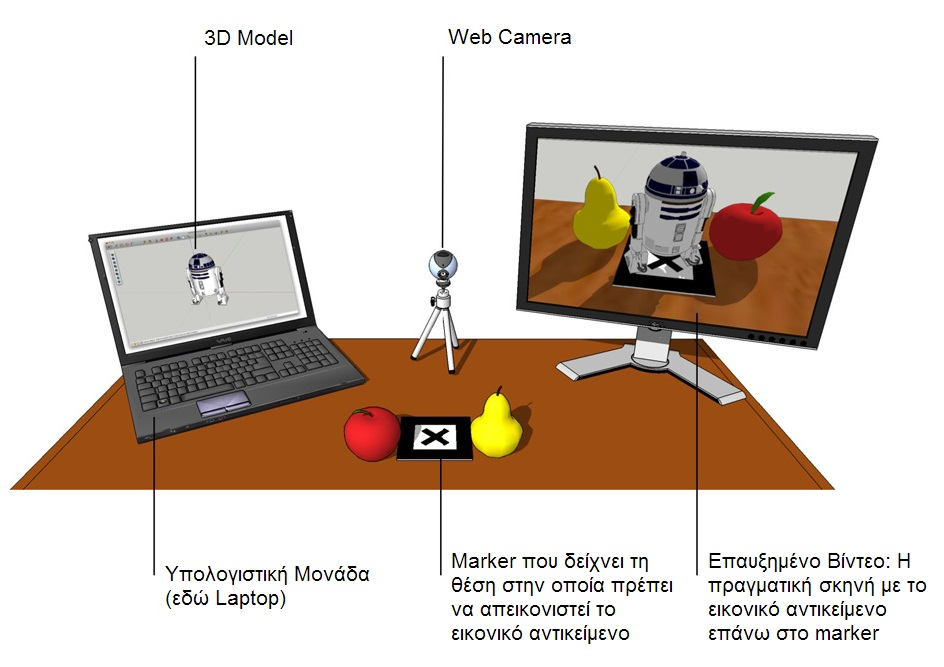
\includegraphics[scale=0.25, angle=0]{Files/Figures/ar_system_example.jpg}
    \caption[Παράδειγμα εγκατάστασης ενός συστήματος επαυξημένης πραγματικότητας ]{ Παράδειγμα εγκατάστασης ενός συστήματος επαυξημένης πραγματικότητας \cite{ar_example}}
    \label{fig:ar_example}
\end{figure}


Η κύρια διαδικασία για τη σωστή λειτουργία ενός συστήματος επαυξημένης πραγματκότητας έχει να κάνει με το κομμάτι της ανίχνευσης. Το κομμάτι αυτό ασχολείται με τον υπολογισμό της σχετικής πόζας της κάμερας σε πραγματικό χρόνο. Με τον όρο πόζα (pose) περιγράφουμε τους 6 βαθμούς ελευθερίας της τοποθεσίας ενός αντικειμένου, δηλαδή τη θέση του στον τρισδιάστατο χώρο και τον προσανατολισμό στον τριασδιάστατο χώρο.

Η διαδικασία της ανίχνευσης είναι αυτή που επιτρέπει την προσθήκη εικονικών αντικειμένων σε μία πραγματική σκηνή.
Η βασική διαφορά σε σύγκριση με άλλα εργαλεία επεξεργασίας εικόνας παρατηρείται στο γεγονός ότι στην επαυξημένη πραγματικότητα τα εικονικά αντικείμενα μετακινούνται και περιστρέφονται σε 3 διαστάσεις αντί για 2 όπως γίνεται συνήθως σε εικόνες.  Ο απλούστερος τρόπος εκτίμησης της πόζας είναι η χρήση δεικτών (markers). 
Ωστόσο, το μαθηματικό μοντέλο ( προβολική γεωμετρία) πίσω από τις μεθόδους υπολογισμού της πόζας είναι το ίδιο. 

Παρόμοια προβλήματα βελτιστοποίησης διαμορφώνονται σε διαφορετικές μεθόδους υπολογισμού της πόζας και λύνονται με τις ίδιες μεθόδους βελτιστοποίησης.  
Μπορούμε να θεωρήσουμε ότι οι markers είναι ένας ειδικός τύπος χαρακτηριστικού και επομένως μπορούμε να ορίσουμε μεθόδους με βάση την ανίχνευση markers και μετέπειτα μεθόδους με βάση την ανίχνευση χαρακτηριστικών, καθώς και υβριδικές μεθόδους. Στη συγκεκριμένη διπλωματική εργασία θα επικεντρωθούμε σε συστήματα επαυξημένης πραγματικότητας που βασίζονται σε markers.

Συνήθως η καταγραφή της εικόνας δεν είναι σημαντικό κομμάτι στην επαυξημένη πραγματικότητα. Συνήθως χρησιμοποιούνται έτοιμες βιβλιοθήκες για το σκοπό αυτό,

Τα εργαλεία και οι βιβλιοθήκες επαυξημένης πραγματικότητας παρέχουν υποστήριξη για την καταγραφή εικόνας και βίντεο. Η διαδικασία τηςα απεικόνισης ζωγραφίζει την εικονική εικόνα πάνω στην εικόνα του βίντεο. Στα γραφικά υπολογιστών, η εικονική σκηνή προβάλλεται πάνω στο επίπεδο της εικόνας χρησιμοποιώντας μία εικονική κάμερα και αυτή η προβολή απεικονίζεται στο τέλος. 

Απαιτείται ουσιαστικά η χρήση μίας εικονικής κάμερας που είναι παρόμοια με τη πραγματική κάμερα του συστήματος. Με αυτό τον τρόπο τα εικονικά αντικείμενα προβάλλονται στη σκηνή με τον ίδιο τρόπο με τον οποίο θα προβάλλονταν πραγματικά αντικείμενα και το αποτέλεσμα είναι γεωμετρικά πειστικό. Για να μπορέσουμε να μιμηθούμε τις ιδιότητες της πραγματικής κάμερας, το σύστημα πρέπει να ξέρει τα οπτικά χαρακτηριστικά της κάμερας. Η διαδικασία κατά την οποία προσδιορίζονται αυτά τα χαρακτηριστικά ονομάζεται βαθμονόμηση κάμερας.

Η βαθμονόμηση της κάμερας μπορεί να είναι μέρος του συστήματος επαυξημένης πραγματικότητας ή ξεχωριστή διαδικασία. Πολλές βιβλιοθήκες παρέχουν εργαλεία βαθμονόμησης, όπως για παράδειγμα οι βιβλιοθήκες ArUco, ALVAR, ARToolkit.


Ωστόσο για τη διαδικασία της βαθμονόμησης μπορούν να χρησιμοποιηθούν και τρίτα εργαλεία βιβλιοθηκών όπως το Matlab ή η OpenCV. 

Στην εργασία αυτή αφού περιγράψουμε τη διαδικασία της βαθμονόμησης, θεωρούμε ότ έχουμε πάντα μία σωστά βαθμονομημένη κάμερα για την ανάπτυξη της εφαρμογής μας.

Η ποικιλία των συσκευών οι οποίες υποστηρίζουν συστήματα επαυξημένης πραγματικότητας είναι μεγάλη και περιλαμβάνει σταθερούς και φορητούς υπολογιστές, tablets, κινητά και άλλες υπολογιστικές μονάδες. Ανάλογα με την εφαρμογή, μπορεί να αξιοποιηθεί η ενσωματωμένη κάμερα της συσκευής, μία απλή USC κάμερα, μία Firewire κάμερα ή μία ψηφιακή κάμερα. Μπορεί επίσης να χρησιμοποιηθεί μία συσκευή απεικόνισης που προσαρτάται στο κεφάλι του χρήστη(HMD), μία συσκευή απεικόνισης οπτικής τεχνολογίας ή η ίδια η οθόνη της υπολογιστικής μονάδας. Επίσης μπορεί το σύστημα να προβάλλει την επαυξημένη σκηνή στον πραγματικό κόσμο\cite{jones2013illumiroom} ή να χρησιμοποιηθεί μια στερεοσκοπική συσκευή απεικόνισης. Η κατάλληλη εγκατάσταση εξαρτάται από την εφαρμογή και το περιβάλλον στο οποίο αναπτύσσεται.









Ο συνδυασμός πραγματικών και εικονικών εικόνων σε μία συγχωνευμένη εικόνα παρουσιάζει τεχνικές δυσκολίες για τους σχεδιαστές εφαρμογών επαυξημένης πραγματικότητας.  Το ερώτημα, στο οποίο καλούνται να απαντήσουν, έχει να κάνει με το πώς θα πραγματοποιηθεί η συνένωση των δύο εικόνων. Στην ενότητα αυτή παρουσιάζονται τα είδη τεχνολογιών θέασης της επαυξημένης σκηνής \cite{azuma1997} \cite{Vallino1998}  \cite{azuma2001}.





-Head-Worn Displays (HWDs)
Οι συσκευές αυτές, γνωστές ως Head-Worn Displays (HWD) ή Head-Attached Displays, φοριούνται στο κεφάλι του χρήστη ή σε κάποιο μέρος του κεφαλιού. Στις παρακάτω παραγράφους περιγράφονται οι κυριότερες κατηγορίες των συσκευών αυτών.\cite{barfield2001fundamentals}


Στην επαυξημένη πραγματικότητα υπάρχουν δύο βασικές κατηγορίες συστημάτων απεικόνισης που αξιοποιούν τα HMDs ως μέσο για την οπτική διεπαφή. 

Επιτυγχάνεται τοποθετώντας οπτικούς μπροστά από τα μάτια του χρήστη. Κάθε σύστημα έχει συγκεκριμένα πλεονεκτήματα και μειονεκτήματα, που σχετίζονται με το σχεδιασμό μιας εφαρμογής και είναι απαραίτητο  να θεωρήσουμε όλες τις παραμέτρους πριν την υλοποίηση του συστήματος AR.Αξίζει να σημειωθεί ότι τα non-immersive HMDs μπορεί να είναι μονοσκοπικά ή στερεοσκοπικά. Οι διαφορές ανάμεσα τους πρέπει να εξεταστούν όταν γίνεται η επιλογή του σχεδιασμού με βάση ένα optical based system. Οι οπτικές προσεγγίσεις είναι απλούστερες και φθηνότερες. Ο κόσμος φαίνεται μέσα από οπτικούς combiners,οπότε υπάρχει μόνο ένα video stream να ανησυχούμε. Στα see-through systems η μόνη διαθέσιμη πληροφορία είναι η θέση της κεφαλής του χρήστη που προέρχεται από έναν head tracker. 



Για την ενίσχυση της "εμβύθισης" του χρήστη χρειάζονται διάφορες τεχνολογίες απεικόνισης της επαυξημένης σκηνής. Τα HMDs έχουν ευρεία χρήση σε εφαρμογές εικονικής πραγματικότητας. Ένα σύστημα Head-Mounted Display (HMD) είναι μία συσκευή που προσαρτάται στο κεφάλι του χρήστη και συνδυάζει την εικόνα του πραγματικού κόσμου με εικονικά αντικείμενα, μέσω χρήσης οπτικής ή βίντεο τεχνολογίας. 
Στο πεδίο της επαυξημένης πραγματικότητας χρησιμοποιούνται 2 είδη HMD. Συγκεκριμένα τα video see-through and optical see-through. Ο όρος “see-through” προέρχεται από την ανάγκη του χρήστη να μπορεί να βλέπει τον πραγματικό κόσμο που βρίσκεται μπροστά του, ακόμα και όταν φοράει το HMD.

 
\textbf{Optical See-Through Displays}


Η τεχνολογία αυτή βασίζεται στη δημιουργία ενός συστήματος παρουσίασης το οποίο προσαρτάται στο κεφάλι του χρήστη (optical see-through HMDs) που απαιτεί την τοποθέτηση "οπτικών συνδυαστών" (συνήθως ημιδιαπερατών και ημιανακλαστικών κάτοπτρων ) μπροστά από τα μάτια του χρήστη, που του επιτρέπουν να δει τόσο το πραγματικό περιβάλλον γύρω του, όσο και τα εικονικά αντικείμενα που παράγονται από τον υπολογιστή. 
Τα εικονικά αντικείμενα ανακλούνται μέσω των κατόπτρων από τις οθόνες που είναι προσαρτημένες στο κεφάλι του, με βάση την τρέχουσα θέση του, όπως φαίνεται στην εικόνα ~\ref{fig:videoseethrough} ).  Επομένως, όταν οι χρήστες μετακινούν τα κεφάλια τους, τα εικονικά αντικείμενα διατηρούν τη θέση τους στον κόσμο σαν να ήταν κομμάτι του πραγματικου περιβάλλοντος.



Τα optical see-through συστήματα δε χρησιμοποιούν καθόλου την είσοδο του σήματος βίντεο, με αποτέλεσμα ο χρήστη να βλέπει το πραγματικό περιβάλλον, και όχι μία αναπαράσταση μέσω βίντεο, πετυχαίνοντας την αξιοποίηση της υψηλής ανάλυσης του πραγματικού κόσμου όπως τον παρατηρεί ο χρήστης. Ουσιαστικά, η συγχώνευση του πραγματικού κόσμου με την εικονική επαύξηση γίνεται οπτικά μπροστά από το χρήστη \cite{Vallino1998} . Αυτή η τεχνολογία είναι παρόμοια με τα  heads up displays (HUD) που χρησιμοποιούνται στα cockpits μαχητικών αεροσκαφών και παρουσιάστηκαν στην προηγούμενη ενότητα~\ref{sec:apps}

Επιπλέον παρουσιάζουν ορισμένα πλεονεκτήματα. Αρχικά θεωρούνται ασφαλή διότι οι χρήστες μπορούν να δουν τη πραγματική σκηνή που βρίσκεται μπροστά τους, ακόμα και αν υπάρξει σφάλμα στην παροχή ισχύος, με αποτέλεσμα η συγκεκριμένη τεχνολογία να είναι ιδανική για στρατιωτικούς και ιατρικούς σκοπούς. Ωστόσο, κι άλλες συσκευές εισόδου όπως κάμερες είναι απαραίτητες για αλληλεπίδραση και registration. Επιπλέον παρουσιάζουν χαμηλό κόστος, και δεν επηρεάζονται από το πρόβλημα της παράλλαξης το οποίο δημιουργεί μία διαφορά ως προς τη θέση των ματιών και της κάμερας \cite{krevelen2010} .


Εφόσον οι χρήστες βλέπουν την πραγματική σκηνή, το εικονικό μέρος είναι ο μόνος λόγος που προκαλείται καθυστέρηση(lag). Για τον ίδιο λόγο, η ποιότητα της σκηνής της προβολής του κόσμου είναι πολύ καλύτερη από την αναπαράσταση μέσω βίντεο. Επομένως η χρήση ενός see-through system εξαλείφει το πρόβλημα της καθυστέρησης του συστήματος και βελτιώνει την ποιότητα προβολής της επαυξημένης σκηνής. 


Ωστόσο πέρα από πλεονεκτήματα, ο συνδυασμός εικονικών αντικειμένων ολογραφικά μέσα από κάτοπτρα και φακούς δημιουργεί και μειονεκτήματα, καθώς μειώνεται η φωτεινότητα, αλλά και η αίσθηση "εμβύθισης" του χρήστη. Επομένως η συγκεκριμένη τεχνική φαίνεται ακατάλληλη για εξωτερική χρήση. Παράλληλα, μία σημαντική παράμετρος, αυτή του πεδίου όρασης του χρήστη (field-of-view) περιορίζεται και μπορεί να προκληθεί ψαλιδισμός των εικονικών εικόνων στα άκρα των ανακλαστήρων. Τέλος, η απόκρυψη των πραγματικών αντικειμένων (occlusion) είναι δυσκολότερη επειδή το φως συνδυάζεται πάντα με την εικονική εικόνα. 

Επιπλέον το γεγονός ότι δεν υπάρχει σήμα βίντεο, αφού δεν υπάρχει κάμερα. Επομένως οι αισθητήρες θέσης μέσα στο HMD είναι ο μόνος τρόπος να εξάγουμε πληροφορίες της πόζας για λόγους registration. Αυτό έχει σαν συνέπεια τη μείωση της ακρίβειας του registration, αν η επιλεγμένη μέθοδος head tracking που χρησιμοποιείται δεν είναι απόλυτα ακριβής \cite{Malik2002} .

H ποιότητα της εικονικής επαύξησης είναι συνήθως χαμηλή, αφού ο μικρός οπτικός συνδυαστής μπροστά από το μάτι του χρήστη είναι χαμηλής ανάλυσης. Έτσι περιορίζεται η εμφάνιση την εμφάνιση των λεπτομερειών των γραφικών που προβάλλονται στην έξοδο. Η ποιότητα των εικονικών αντικειμένων περιορίζεται από την ταχύτητα επεξεργασίας και τις γραφικές ικανότητες του συστήματος επαύξησης. Επομένως η δημιουργία πειστικών επαυξήσεων γίνεται δυσκολότερη αφού ο πραγματικός κόσμος θα εμφανίζεται κανονικά, σε αντίθεση με τα εικονικά αντικείμενα που θα εμφανίζονται pixilated. Αν ένα σύστημα επαυξημένης πραγματικότητας απαιτεί εικονικά αντικείμενα με γραφικά υψηλής ανάλυσης, τότε προτιμώνται συνήθως συστήματα video see-through ή monitor-based \cite{Mcdonald2003} . 


\begin{figure}[H]
    \centering
    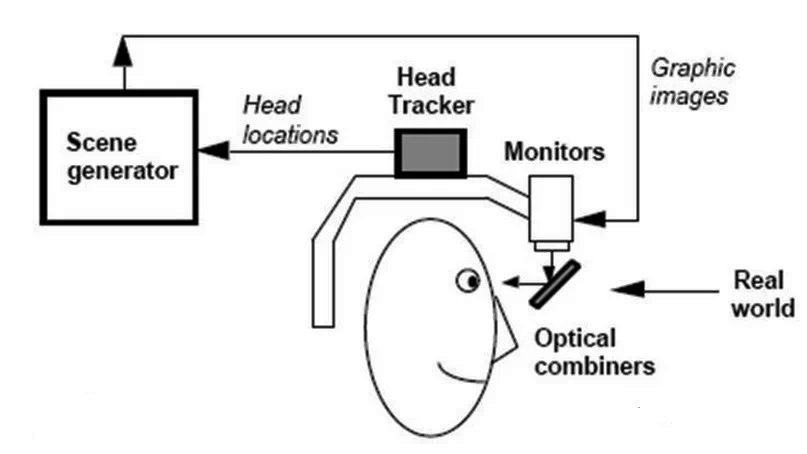
\includegraphics[scale=0.7, angle=0]{Files/Figures/optical.jpg}
    \caption[Διάγραμμα συστήματος Optical See-Through Display \cite{azuma1997}]{ Διάγραμμα συστήματος Optical See-Through Display \cite{azuma1997}}
    \label{fig:opticalseethrough}
\end{figure}



\textbf{Video See-Through Displays}

Τα HMDs που χρησιμοποιούν βίντεο τεχνολογία (video see-through HMDs), συνδυάζουν ένα «κλειστό» HMD (closed-view HMD) και μία ή δύο βιντεοκάμερες προσαρτημένες στο κεφάλι του χρήστη, όπως φαίνεται στην εικόνα ~\ref{fig:videoseethrough} . Η σκηνή του πραγματικού κόσμου καταγράφεται από τις βιντεοκάμερες, οι οποίες του παρέχουν τη δυνατότητα να βλέπει τον πραγματικό κόσμο. Με αυτό τον τρόπο, ο χρήστης δε βλέπει τον πραγματικό κόσμο απευθείας, αλλά αντίθετα βλέπει μόνο αυτό που απεικονίζεται στις μικρές οθόνες στο εσωτερικό του HMD.  

 

Το πλεονέκτημα των συστημάτων τέτοιου τύπου παρατηρείται στο ότι κατά τη καταγραφή της πραγματικής σκηνής μέσω βίντεο, μπορούν να εξαχθούν πληροφορίες για τη σκηνή. Οι ψηφιοποιημένες εικόνες επιτρέπουν την ανίχνευση της κίνησης του κεφαλιού του χρήστη παρέχοντας μεγαλύτερη ακρίβεια κατά τη διαδικασία του tracking της θέσης του κεφαλιού και επομένως οδηγεί σε πιο ακριβές registration. Επιπλέον η απεικόνιση του βίντεο είναι συνήθως υψηλής ανάλυσης και δίνεται η δυνατότητα να απεικονιστούν τα εικονικά αντικείμενα με λεπτομερή γραφικά σε συνδυασμό με το βίντεο εισόδου.Συνεπώς, αυξάνεται η ρεαλιστικότητα και η εμβύθιση του χρήστη που μπορεί να προσφέρει ο επαυξημένος κόσμος \cite{krevelen2010} .


Αυτή η διαδικασία συγχώνευσης προσθέτει ωστόσο καθυστερήσεις στο σύστημα. Οι καθυστερήσεις του συστήματος λόγω της καταγραφής, της επεξεργασίας, της επαύξησης και της απεικόνισης σε κάθε frame του βίντεο μεταφράζεται σε lag που καταλαβαίνει ο χρήστης με αποτέλεσμα να χάνεται η αίσθηση της εμβύθισης. Αυτό είναι ένα μειονέκτημα στα συστήματα video see-through technology που δεν μπορεί να αποφευχθεί αλλά μπορεί να ελαχιστοποιηθεί. Μειονεκτήματα εντοπίζονται επίσης στη χαμηλή ανάλυση απεικόνισης του πραγματικού κόσμου, στο περιορισμένο field-of-view (αν και μπορεί να αυξηθεί εύκολα), και τον αποπροσανατολισμό των χρηστών λόγω της παράλλαξης (eye-offset) λόγω της θέσης της κάμερας σε μία απόσταση από τη πραγματική θέση των ματιών του χρήστη. Τέλος, μία μεγάλη διαφορά ανάμεσα στις κάμερες και τα μάτια του χρήστη, μπορεί να ελλατώσει την αίσθηση της εμβύθισης, αφού τα πάντα στις σκηνές που καταγράφονται θα μετατοπιστούν ψηλότερα ή χαμηλότερα από εκεί που θα έπρεπε να είναι(ως προς την κανονικό επίπεδο της θέσης των ματιών) \cite{Malik2002} . 



\begin{figure}[H]
    \centering
    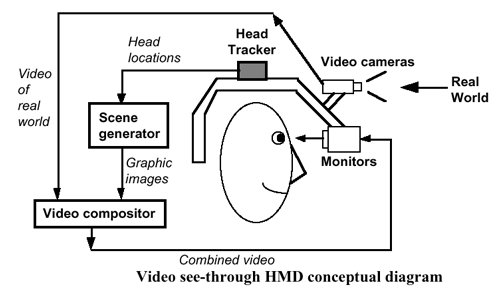
\includegraphics[scale=0.8, angle=0]{Files/Figures/videoseethrough.jpg}
    \caption[Διάγραμμα συστήματος Video See-Through Display \cite{azuma1997}]{ Διάγραμμα συστήματος Video See-Through Display \cite{azuma1997}}
    \label{fig:videoseethrough}
\end{figure}


\textbf{Monitor-based Systems}


Πέρα όμως από τις συσκευές τεχνολογίας HMD, υπάρχουν και συσκεύες απεικόνισης σε οθόνη με χρήση βίντεο-τεχνολογίας. Οι συσκευές αυτές απεικονίζουν τις επαυξημένες σκηνές σε μία κοινή οθόνη, κάνοντας χρήση της επεξεργασίας εικόνας και της μίξης του εικονικού με το πραγματικό. Η απλούστερη προσέγγιση ενός monitor-based συστήματος απεικόνισης, φαίνεται στο~\ref{fig:monitor} .

Το είδος αυτό της επαυξημένης πραγματικότητας αποτελεί μία από τις πιο απλές και αποδοτικές λύσεις, καθώς απαιτεί έναν τυπικό ηλεκτρονικό υπολογιστή και  και μία βιντεοκάμερα USB ή Firewire. Ωστόσο αυτή η απλότητα προκαλεί συνέπειες στον τομέα της εμβύθισης του χρήστη σε περιβάλλοντα επαυξημένης πραγματικότητας, λόγω του σχετικά μικρού μεγέθους της οθόνης και του συνακόλουθου μικρού οπτικού πεδίου. Το σύστημα επαύξησης μπορεί να χρησιμοποιήσει τεχνικές με βάση την όραση υπολογιστών για να υπολογίσει τις πληροφορίες της πόζας(θέση και προσανατολισμός) του χρήστη για σκοπούς registration (ανιχνεύοντας χαρακτηριστικά ή πρότυπα για παράδειγμα).

Ακόμη, μειονέκτημα αποτελεί η ποιότητα της εικόνας, καθώς αυτή περιορίζεται από την ανάλυση της κάμερας. Προφανώς, το να βλέπει κάποιος τον πραγματικό κόσμο μέσα από τη μικρή οθόνη ενός υπολογιστή περιορίζει το ρεαλισμό και την φορητότητα του επαυξημένου κόσμου. Επιπλέον, εφόσο κάθε frame της κάμερας χρειάζεται επεξεργασία από το σύστημα επαύξησης, μπορεί να καταγραφεί καθυστέρηση λόγω του χρόνου από τη στιγμή που καταγράφεται η πραγματική σκηνή, μέχρι να απεικονιστεί η τελική επαυξημένη εικόνα. 




\begin{figure}[H]
    \centering
    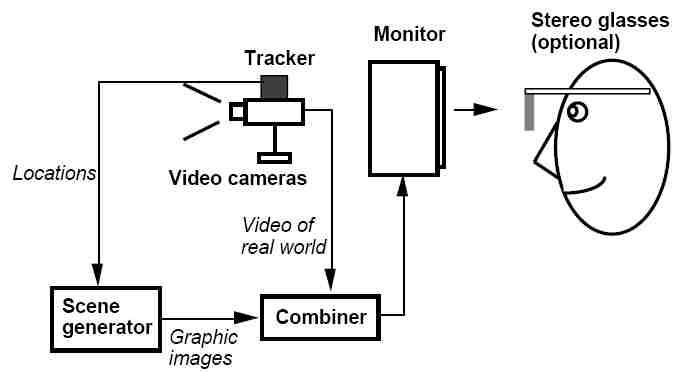
\includegraphics[scale=0.8, angle=0]{Files/Figures/monitor.jpg}
    \caption[Διάγραμμα συστήματος Monitor Display \cite{azuma1997}]{ Διάγραμμα συστήματος Monitor Display \cite{azuma1997}}
    \label{fig:monitor}
\end{figure}


\begin{figure}[H]
    \centering
    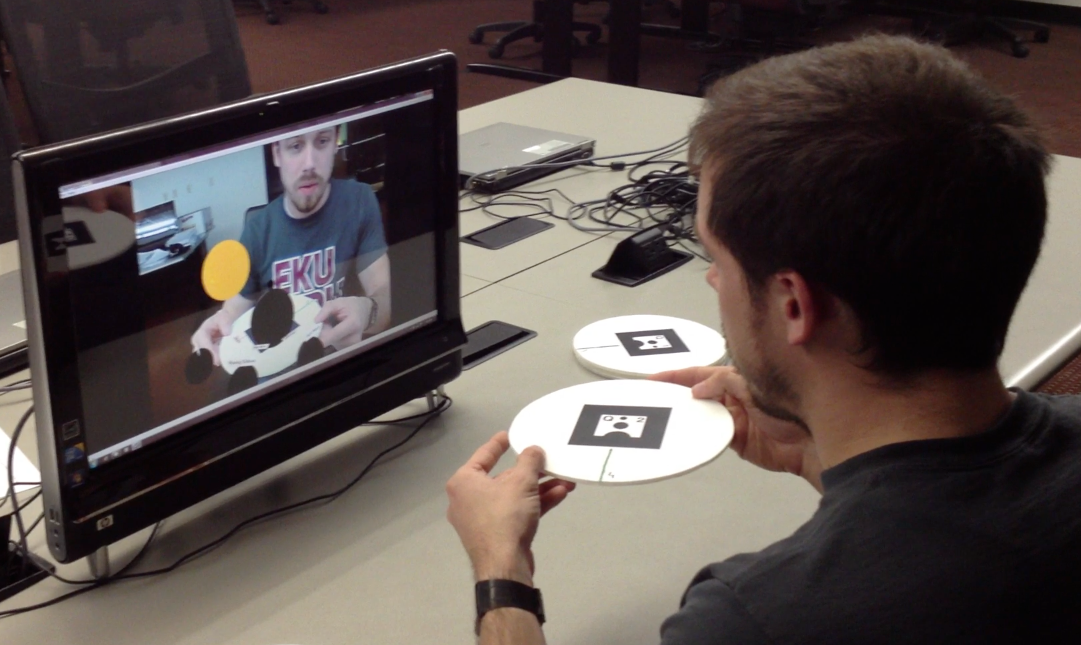
\includegraphics[scale=0.2, angle=0]{Files/Figures/monitor_example.png}
    \caption[Παράδειγμα εφαρμογής μέσω συσκευής απεικόνισης σε
οθόνη \cite{monitor_ar} .]{ Παράδειγμα εφαρμογής μέσω συσκευής απεικόνισης σε
οθόνη \cite{monitor_ar} .}
    \label{fig:monitor_example}
\end{figure}


\textbf{Φορητές Συσκευές}


Οι συσκευές αυτές, ευρέως γνωστές ως Handheld Displays (HDs), περιλαμβάνουν μία οθόνη, μέσω της οποίας είναι δυνατή η θέαση της επαυξημένης σκηνής, και είναι φορητές, μικρού μεγέθους, έτσι ώστε ο χρήστης να μπορεί να τις κρατήσει στο χέρι του και να τις μεταφέρει μαζί του. 

Τέτοιες συσκευές είναι τα κινητά τηλέφωνα – και συγκεκριμένα τα «έξυπνα» κινητά τηλέφωνα, γνωστά ως smartphones – τα tablet PCs και οι – λιγότερο χρησιμοποιούμενοι πλέον – προσωπικοί ψηφιακοί οδηγοί PDAs (Personal Digital Assistants). 

Στη μεγάλη πλειονότητα των εφαρμογών επαυξημένης πραγματικότητας που προορίζονται για φορητές συσκευές χειρός, η βιντεοκάμερα «αιχμαλωτίζει» τη ζωντανή εικόνα του πραγματικού περιβάλλοντος, η οποία επαυξάνεται με επιπρόσθετες γραφικές πληροφορίες πριν την απεικόνισή της στην οθόνη. 

Μέσω των συσκευών αυτών, ο χρήστης δεν «βυθίζεται» στο επαυξημένο περιβάλλον, αλλά το παρακολουθεί μέσω της οθόνης της συσκευής του, γεγονός το οποίο θα μπορούσε να θεωρηθεί ως μειονέκτημα. 

Επίσης, η συνήθως χαμηλή επεξεργαστική ισχύ και μνήμη τους, μπορεί να προκαλέσει καθυστερήσεις κατά την εκτέλεση της εφαρμογής. Ωστόσο οι συσκευές αυτές παρουσιάζουν το πλεονέκτημα του μικρότερου μεγέθους και βάρους \cite{wagner2007handheld} \cite{arth2015history} .

Τα τελευταία χρόνια έχουν αναπτυχθεί και σύγχρονα συστήματα απεικόνισης όπως ειδικοί φακοί επαφής, ωστόσο δε θα αναφέρουμε περισσότερα για τη συγκεκριμένη τεχνολογία.





\section{Marker-based Tracking}
%MONO FIDUCIAL MARKER TRACKING

%eisagogi enotitas
While some approaches seek natural features such as key points or textures,fiducial markers are still an attractive approach because they are easy to detect and high speed, as well as precision may be achieved.


Σε αυτό το κεφάλαιο γίνεται μία εισαγωγή στις μαθηματικές έννοιες της επαυξημένης πραγματικότητας, στις μεθόδους που χρησιμοποιούνται και στην αναγνώριση δεικτών.  
In this chapter, we review prior work in the field of augmented reality from which our research draws upon. We start by providing an introduction to the mathematical concepts of augmented reality, and describe how they relate to the registration problem. We then present a brief survey of various proposed solutions to the registration problem in the current augmented reality literature. We conclude by briefly describing some open issues.




Η επαυξημένη πραγματικότητα παρουσιάζει πληροφορίες στα πλαίσια του πραγματικού κόσμου. Για να συμβεί αυτό, το σύστημα πρέπει να γνωρίζει που βρίσκεται ο χρήστης και προς τα που κοιτά σε κάθε χρονική στιγμή. Συνήθως ο χρήστης εξερευνεί το περιβάλλον μέσα από μία οθόνη που απεικονίζει την εικόνα που καταγράφει η κάμερα μαζί με την επαυξημένη πληροφορία.  
Επομένως, το σύστημα χρειάζεται πρακτικά να ξέρει τη θέση και τον προσανατολισμό της κάμερας, έτσι ώστε να απεικονίσει τα εικονικά αντικείμενα στη σωστή θέση. Αυτή η διαδικασία ονομάζεται tracking και αναφέρεται στον υπολογισμό της σχετικής πόζας(pose) της κάμερας (θέση και προσανατολισμός) σε πραγματικό χρόνο και είναι ένα από τα βασικότερα μέρη ανάπτυξης εφαρμογών επαυξημένης πραγματικότητας.


Οι ερευνητές στα πεδία της όρασης υπολογιστών έχουν αναπτύξει έναν αξιοσημείωτο αριθμό μεθόδων tracking. Οι μέθοδοι αυτές μπορούν να ταξινομηθούν με βάση τον εξοπλισμό που χρησιμοποιείται σε μεθόδους sensor tracking, visual tracking και υβριδικές. Εφόσον στα περισσότερα συστήματα επαυξημένης πραγματικότητας χρησιμοποιείται συνήθως μία κάμερα, οι τεχνικές visual tracking είναι αυτές που παρουσιάζουν μεγαλύτερο ενδιαφέρον, οπότε θα επικεντρωθούμε σε αυτές.


Στα συστήματα visual tracking, η πόζα της κάμερας μπορεί να υπολογιστεί με βάση την παρατήρηση των σκηνών που καταγράφει. Σε ένα άγνωστο περιβάλλον, παρατηρούνται πολλές δυσκολίες, καθώς απαιτείται αρκετός χρόνος προκειμένου να γίνει η συλλογή αρκετών δεδομένων για τον υπολογισμό της πόζας και επιπλέον, η εκτίμηση των υπολογισμών ολισθαίνει με την πάροδο του χρόνου. Καθώς το περιβάλλον δεν είναι γνωστό στο σύστημα, ο προσανατολισμός του άξονα συντεταγμένων επιλέγεται τυχαία, κάτι το οποίο μπορεί να μην είναι ιδιαίτερα βολικό για το χρήστη. Επιπλέον, είναι αδύνατο να υπολογιστεί η σωστή κλίμακα μόνο με βάση τις οπτικές παρατηρήσεις. Μία λύση που θα μπορούσε να ξεπεράσει αυτές τις δυσκολίες, εντοπίζεται στην εισαγωγή ενός ανιχνεύσιμου προκαθορισμένου στόχου στο περιβάλλον και στη χρήση τεχνικών όρασης υπολογιστών για τον εντοπισμό του στη σκηνή. 

Ο στόχος αυτός είναι ουσιαστικά ένας δείκτης ή marker, ένα σημάδι ή μια εικόνα, που μπορεί να εντοπιστεί από ένα υπολογιστικό σύστημα μέσω του βίντεο χρησιμοποιώντας τεχνικές επεξεργασίας εικόνας, αναγνώρισης προτύπων και υπολογιστικής όρασης (π.χ~\ref{fig:marker})). Μόλις εντοπιστεί ένας marker, μπορεί να οριστεί η σωστή θέση και ο προσανατολισμός της κάμερας. Αυτή η προσέγγιση ονομάζεται ανίχνευση βασισμένη σε marker (marker-based tracking) και χρησιμοποιείται ευρύτατα στην επαυξημένη πραγματικότητα.%vale link

\begin{figure}[H]
    \centering
    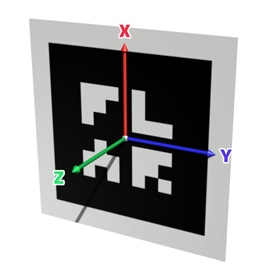
\includegraphics[scale=0.6, angle=0]{Files/Figures/marker-axis.jpg}
    \caption[Παράδειγμα marker]{ Παράδειγμα marker}
    \label{fig:marker}
\end{figure}




Άλλες προσεγγίσεις χρησιμοποιούν ανίχνευση με βάση τον εντοπισμό οπτικών χαρακτηριστικών και εντοπισμό προκαθορισμένων μοντέλων. Στον εντοπισμό με βάση προκαθορισμένα μοντέλα, το σύστημα γνωρίζει εκ των προτέρων τις ιδιότητες ενός μοντέλου ή μέρους της σκηνής (π.χ CAD μοντέλο). Πραγματοποιείται σύγκριση ανάμεσα στα frames που κταγράφονται και γίνεται προσπάθεια να γίνει αντιστοίχηση του μοντέλου με ένα μέρος της σκηνής. Μόλις συμβεί αυτό, μπορεί να υπολογιστεί και η πόζα της κάμερας. Στη διαδικασία feature-based tracking,το σύστημα προσπαθεί να ανιχνεύσει οπτικά χαρακτηριστικά της σκηνής μέσα από τις εικόνες και να γνωρίσει το περιβάλλον με βάση ορισμένες παρατηρήσεις κινήσεων ανάμεσα σε διαδοχικά frames. Αν και η επικρατούσα τάση στην έρευνα σχετικά με το visual tracking τείνει προς το feature-based tracking, που δεν απαιτεί την εκτύπωση και χρήση markers, οι μέθοδοι που βασίζονται σε markers παρουσιάζουν καλύτερες επιδόσεις από τις μεθόδους feature-based σε συγκεκριμένες περιπτώσεις και χρησιμοποιούνται ακόμα πολύ συχνά σε εφαρμογές επαυξημένης πραγματικότητας \cite{wagner2008robust} \cite{rabbi2014applications} .


Η ευρεία χρήση συστημάτων που λειτουργούν με βάση την ανίχνευση markers εξηγείται και από το γεγονός ότι είναι εύκολα στην υλοποίηση και υπάρχουν πολλά διαθέσιμα εργαλεία για την ανάπτυξη τέτοιων εφαρμογών (π.χ ARToolKit \cite{artoolkit}, ALVAR \cite{alvar}, ArUco \cite{aruco}). Τα εργαλεία αυτά αποτελούν μία καλή βάση για να ξεκινήσει κάποιος την ανάπτυξη εφαρμογών επαυξημένης πραγματικότητας. Επιπλέον, οι markers παρέχουν εκτιμήσεις για τη σωστή κλίμακα και βολικές συντεταγμένες για κάθε frame όπως αναφέρθηκε και προηγουμένως. Μπορούν να κωδικοποιήσουν πληροφορίες ή να έχουν απλά ένα ID. Κάτι τέτοιο, επιτρέπει στο σύστημα να επισυνάψει συγκεκριμένα αντικείμενα ή αλληλεπιδράσεις στα markers. Στη συστήματα που χρησιμοποιούν marker-based tracking, απαιτείται η ανίχνευση του marker, η ταυτοποίηση του και ο υπολογισμός της πόζας. 

Στις παρακάτω ενότητες, παρουσιάζεται η διαδικασία υπολογισμού της πόζας ενός δείκτη. Αρχικά παρουσιάζονται περιληπτικά οι βασικές αρχές της προβολικής γεωμετρίας και το μοντέλο κάμερας pinhole. Ύστερα αναλύεται η διαδικασία βαθμονόμησης κάμερας με αποτέλεσμα τον υπολογισμό των παραμέτρων της και ο τρόπος ανίχνευσης ενός marker. Στο τέλος της ενότητας παρουσιάζεται ένας τρόπος αξιοποίησης πολλαπλών markers με στόχο τη βελτίωση της επίδοσης του συστήματος.




\begin{figure}[H]
    \centering
    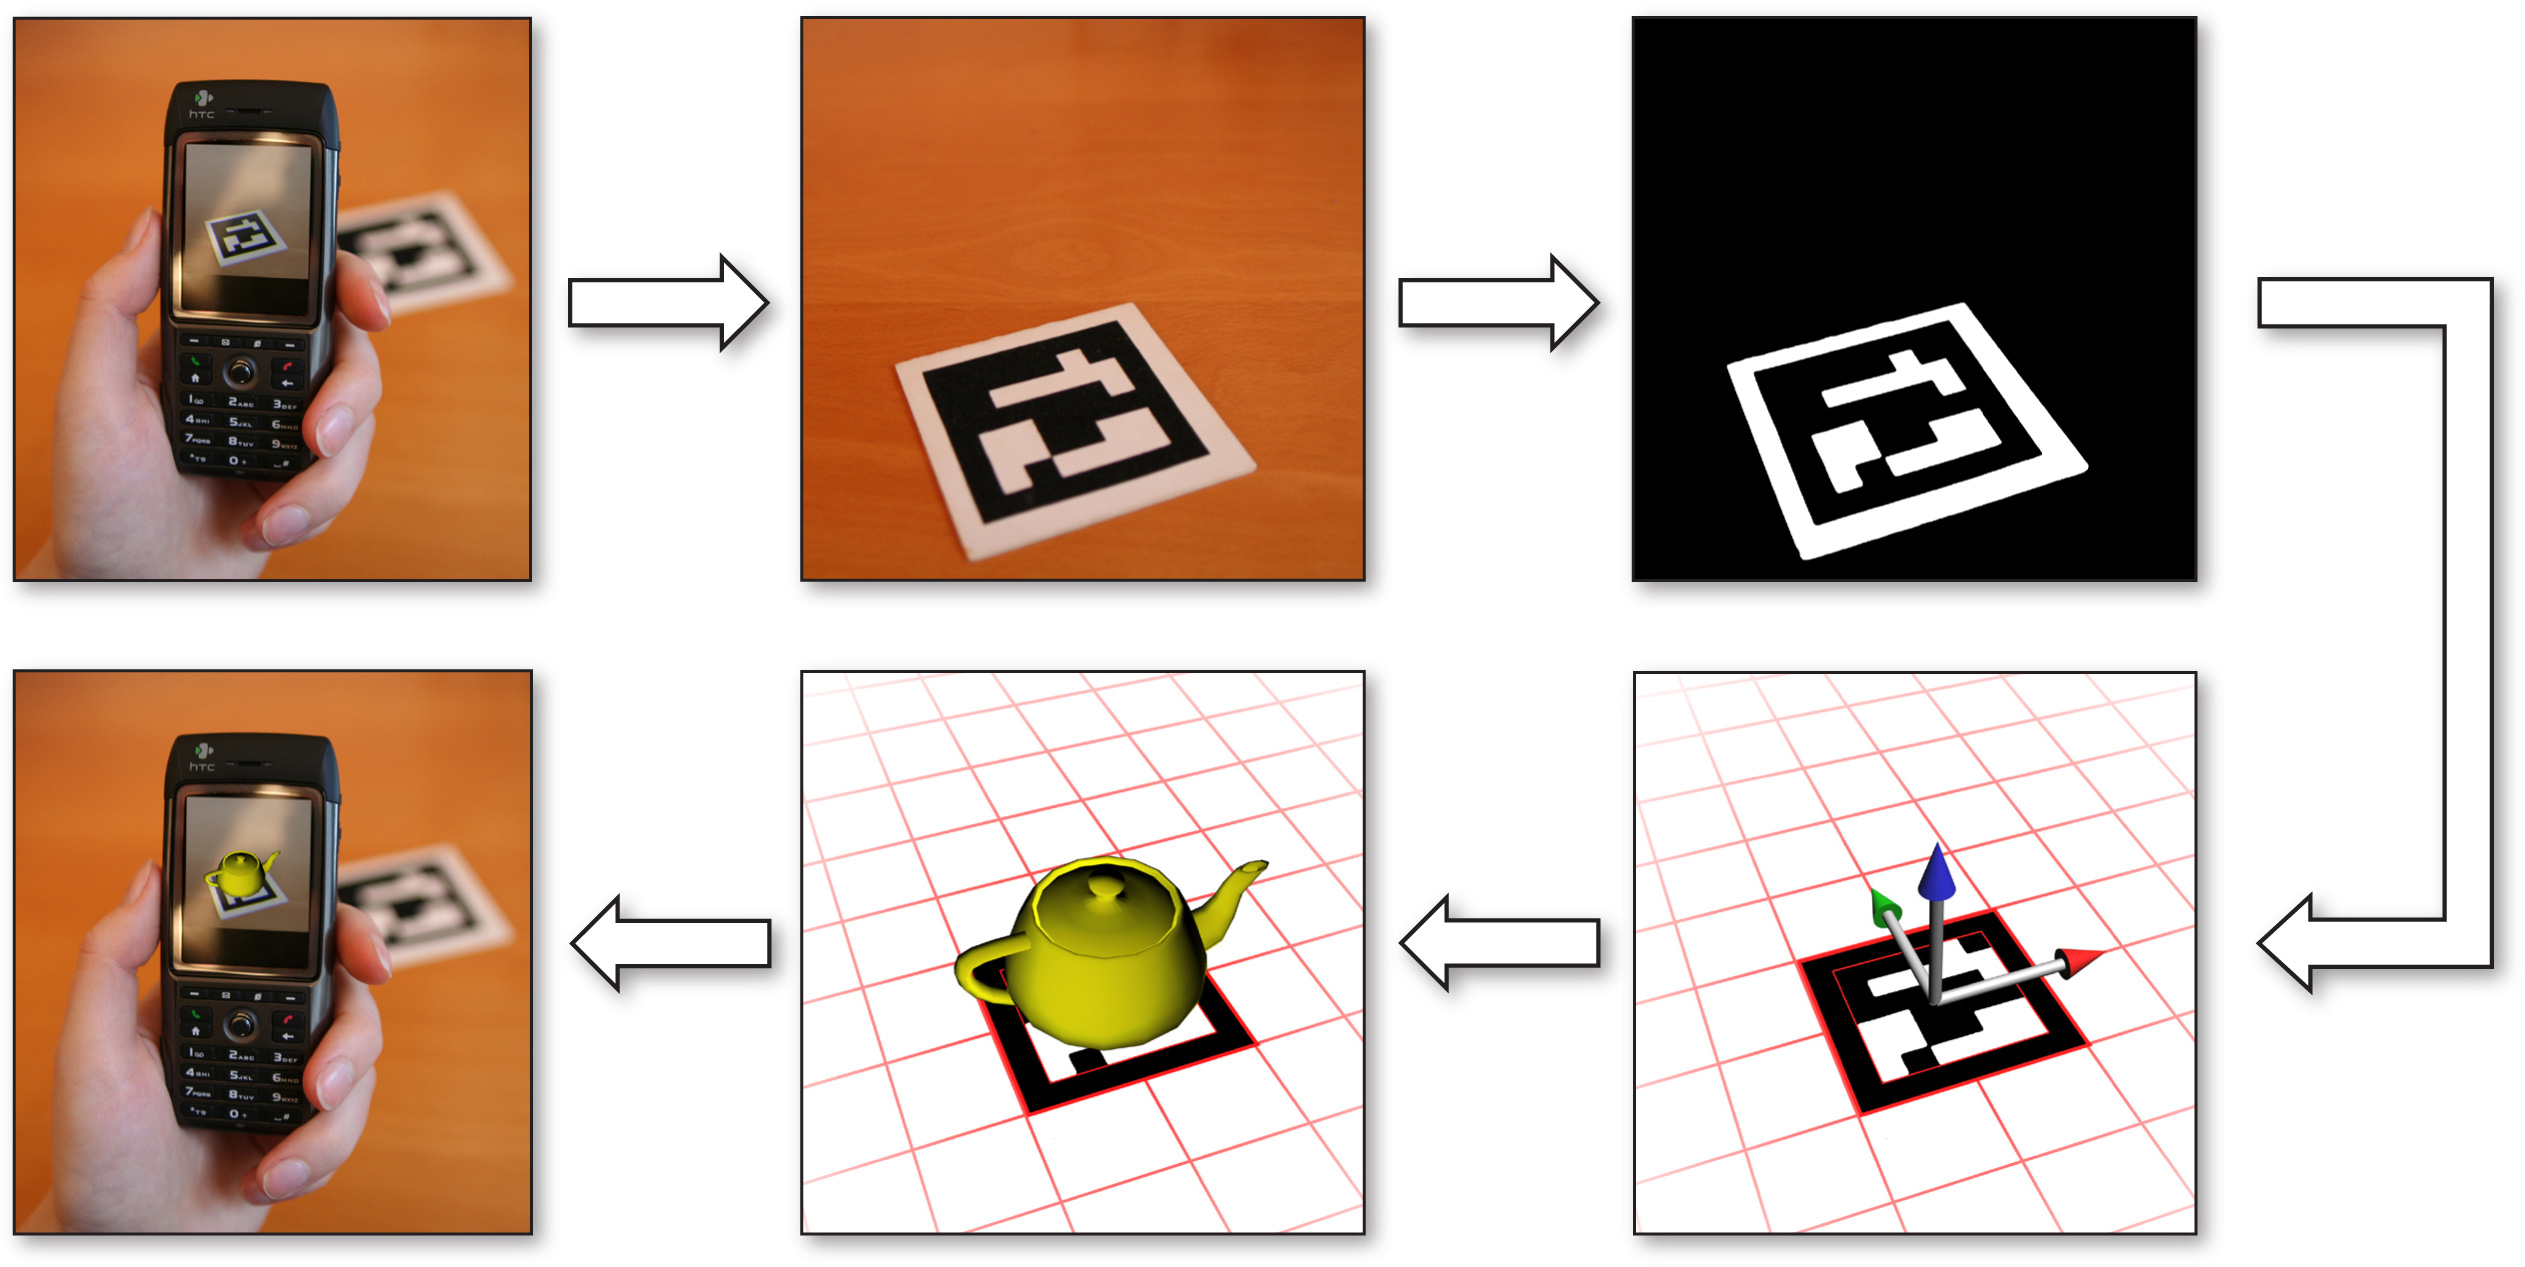
\includegraphics[scale=0.6, angle=0]{Files/Figures/HowMarkersWork.jpg}
    \caption[Παράδειγμα εντοπισμού marker και επαύξησης της σκηνής \cite{howmarkerswork}]{ Παράδειγμα εντοπισμού marker και επαύξησης της σκηνής \cite{howmarkerswork}}
    \label{fig:howmarkerswork}
\end{figure}


Στη συνέχεια του κεφαλαίου θα χρησιμοποιήσουμε ομογενείς συντεταγμένες. Οι ομογενείς συντεταγμένες (homogeneous coordinates) είναι ένα είδος συντεταγμένων που χρησιμοποιείται στην προβολική γεωμετρία, αντίστοιχα με τις καρτεσιανές συντεταγμένες που χρησιμοποιούνται στην ευκλείδεια γεωμετρία. Στα πλεονεκτήματά τους συγκαταλέγονται η δυνατότητα αναπαράστασης όλων των σημείων, ακόμα και των σημείων του απείρου, με πεπερασμένες συντεταγμένες, καθώς και η δυνατότητα έκφρασης ενός προβολικού μετασχηματισμού με τη βοήθεια ενός μόνο πίνακα.

Πιο συγκεκριμένα, έστω ένα σημείο της εικόνας με καρτεσιανές συντεταγμένες \[\begin{bmatrix} x \\ y \end{bmatrix}\]
Το αντίστοιχο σημείο, σε ομογενείς συντεταγμένες μπορεί να αναπαρασταθεί ως: \[\begin{bmatrix} wx \\ wy \\ w\end{bmatrix}=
\begin{bmatrix}x'\\y'\\w\end{bmatrix} , w\neq0 \].

Ομοίως στον 3D χώρο ένα σημείο με καρτεσιανές συντεταγμένες \[\begin{bmatrix} x \\ y \\ z \end{bmatrix}\] μπορεί να αναπαρασταθεί ως: \[\begin{bmatrix} wx \\ wy \\ wz \\ w\end{bmatrix}=
\begin{bmatrix}x'\\y'\\z' \\ w\end{bmatrix} , όπου w\neq0 \].


Παρά το γεγονός ότι μπορεί να χρησιμοποιηθεί ένας οποιοσδήποτε μη μηδενικός αριθμός $w$, συνήθως παίρνουμε $w=1$, ώστε η αλλαγή συστήματος συντεταγμένων να γίνεται ευκολότερα.

Ο παρακάτω πίνακας συνοψίζει την αναπαράσταση των σημείων που θα χρησιμοποιηθεί:




\begin{tabu} to 0.9\textwidth { | X[l] | X[c,m] | X[c,m] | }
   \hline
    & Ευκλείδεια Γεωμετρία & \vspace{0.3cm}Προβολική Γεωμετρία \\[0.5cm]
   \hline
   Σημείο στο 2Δ Χώρο  & $\begin{bmatrix} x \\ y\end{bmatrix}$  & \vspace{0.3cm}$\begin{bmatrix} x \\ y\\1\end{bmatrix}$  \\[1cm]
   \hline
   Σημείο στο 3Δ Χώρο  & $\begin{bmatrix} X \\ Y \\ Z\end{bmatrix}$  & \vspace{0.3cm}$\begin{bmatrix} X \\ Y\\Z\\1\end{bmatrix}$  \\[1cm]
   \hline
\end{tabu}






\subsection{Το Μοντέλο Κάμερας Pinhole}



Στα πεδία της υπολογιστικής όρασης και των γραφικών, το απλούστερο μαθηματικό μοντέλο, το οποίο περιγράφει τη σχέση μεταξύ των συντεταγμένων χώρου ενός αντικειμένου και της προβολής τους στην εικόνα είναι το μοντέλο κεντρικής προβολής. Στην πραγματικότητα, η κεντρική προβολή περιγράφει με ακρίβεια μόνο τη μηχανή σημειακής οπής (pinhole camera), με αποτέλεσμα να αναφέρεται συχνά και ως pinhole camera model \cite{hartley2003multiple} .


Το μοντέλο αυτό, βασίζεται στην θεώρηση ότι όλες οι ακτίνες φωτός περνούν μέσα από μία οπή αμελητέων διαστάσεων και το είδωλο ενός αντικειμένου προβάλλεται πάνω στο επίπεδο μιας εικόνας. Επειδή μέσω της κεντρικής προβολής δημιουργούνται ανεστραμμένες εικόνες \cite{fig:pinhole3}, πολλές φορές καθίσταται βολική η θεώρηση του επιπέδου προβολής μπροστά από την μικροσκοπική οπή, στην ίδια απόσταση που βρισκόταν και προηγουμένως, με αποτέλεσμα η φανταστική αυτή εικόνα να μην είναι ανεστραμμένη. 



\begin{figure}[H]
    \centering
    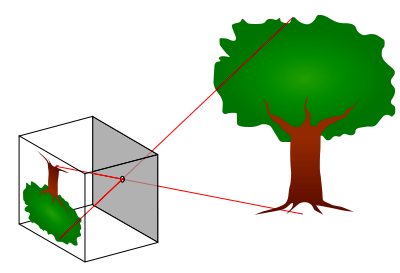
\includegraphics[scale=0.5, angle=0]{Files/Figures/pinhole3.png}
    \caption[Το μοντέλο κεντρικής προβολής (pinhole camera model)]{ Το μοντέλο κεντρικής προβολής (pinhole camera model) \cite{pinhole} .}
    \label{fig:pinhole3}
\end{figure}

%εδω ξεκιναμε να λέμε για τα focal length kai ideal to sensor 
Στις ψηφιακές κάμερες, η εικόνα εγγράφεται στον αισθητήρα της εικόνας με τις συντεταγμένες των στοιχείων του να διαφέρουν από τις ιδανικές συντεταγμένες, αφού η εικόνα της κάμερας εξαρτάται από τα φυσικά χαρακτηριστικά της κάμερας, όπως την εστιακή απόσταση, τον προσανατολισμό του αισθητήρα και το μέγεθος. H εικόνα, λοιπόν, η οποία δεν αποτελεί μία αυστηρά κεντρική προβολή, λόγω ποικίλων σφαλμάτων που οφείλονται στους φακούς, στην ατμόσφαιρα, κ.λπ., προσεγγίζεται γεωμετρικά από το μοντέλο αυτό, στο πλαίσιο της όρασης υπολογιστών. 

Το σχήμα~\ref{fig:pinhole2} δείχνει το μοντέλο κάμερας pinhole. 



%περιγραφη της εικονας γεωμετρικα

\begin{figure}[H]
    \centering
    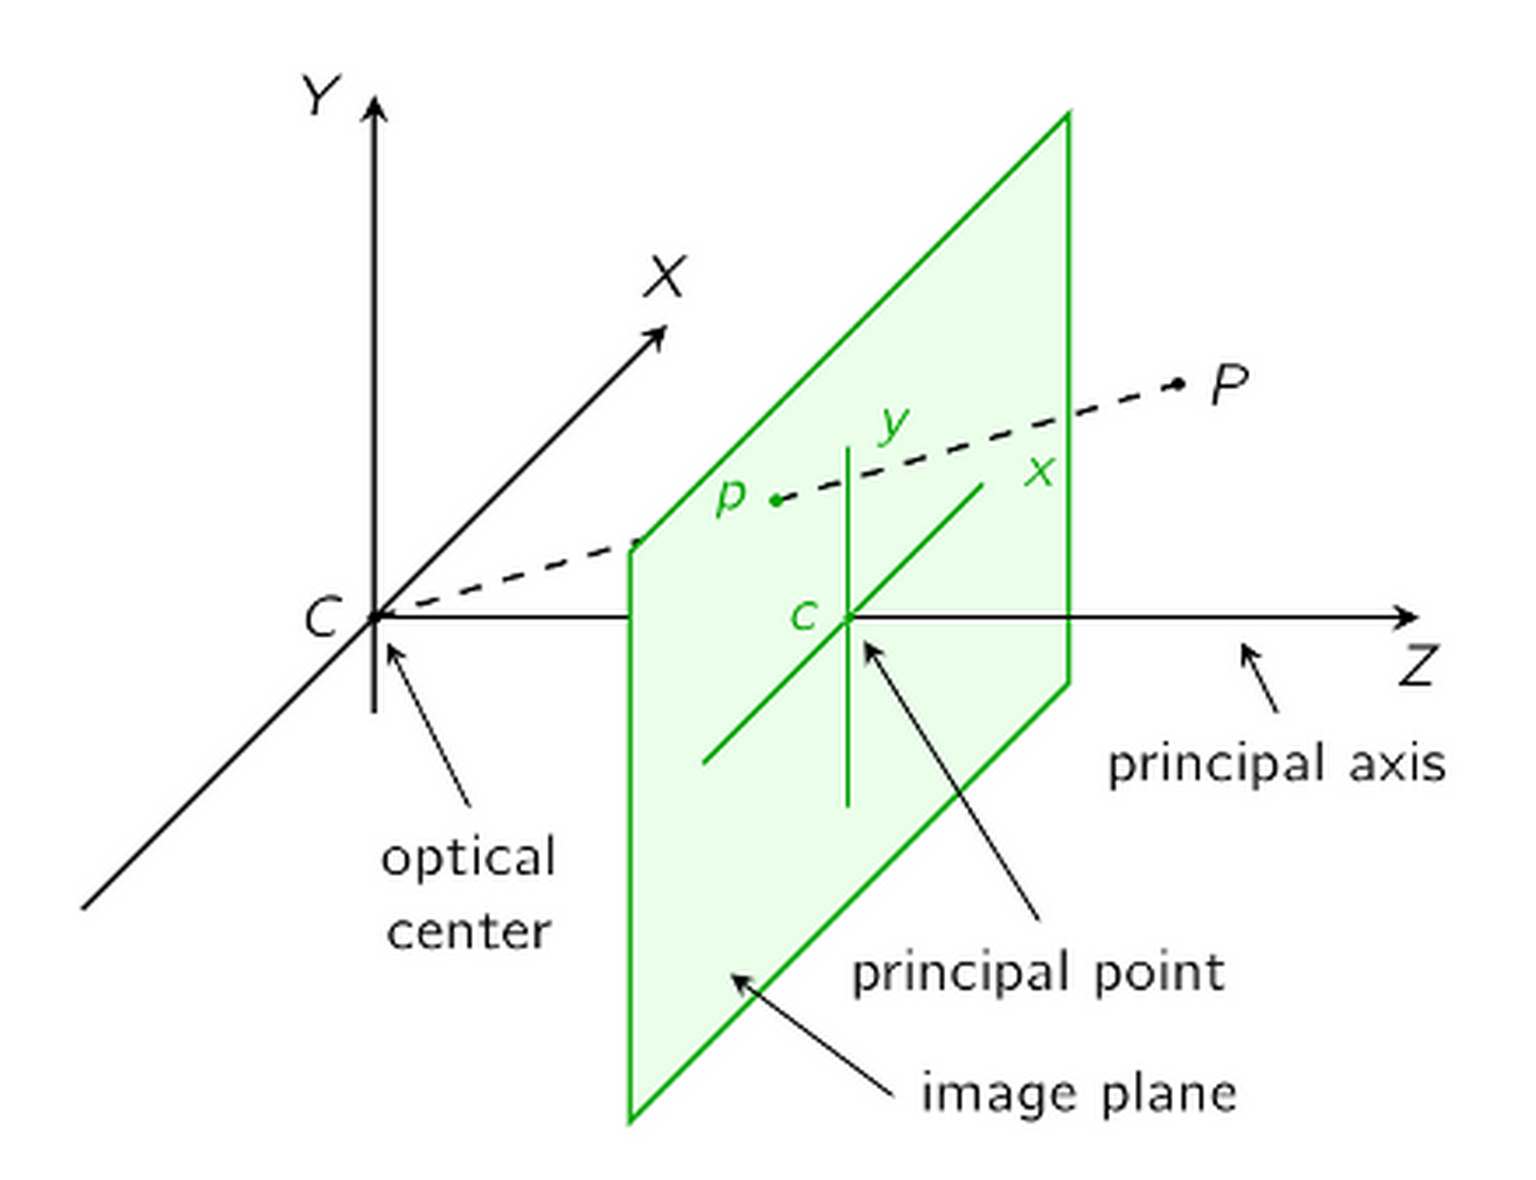
\includegraphics[scale=0.5, angle=0]{Files/Figures/pinhole1.png}
    \caption[Το μοντέλο κεντρικής προβολής στις 3 διαστάσεις (pinhole camera model)]{ Το μοντέλο κεντρικής προβολής (pinhole camera model) \cite{pinhole} .}
    \label{fig:pinhole1}
\end{figure}


\begin{figure}[H]
    \centering
    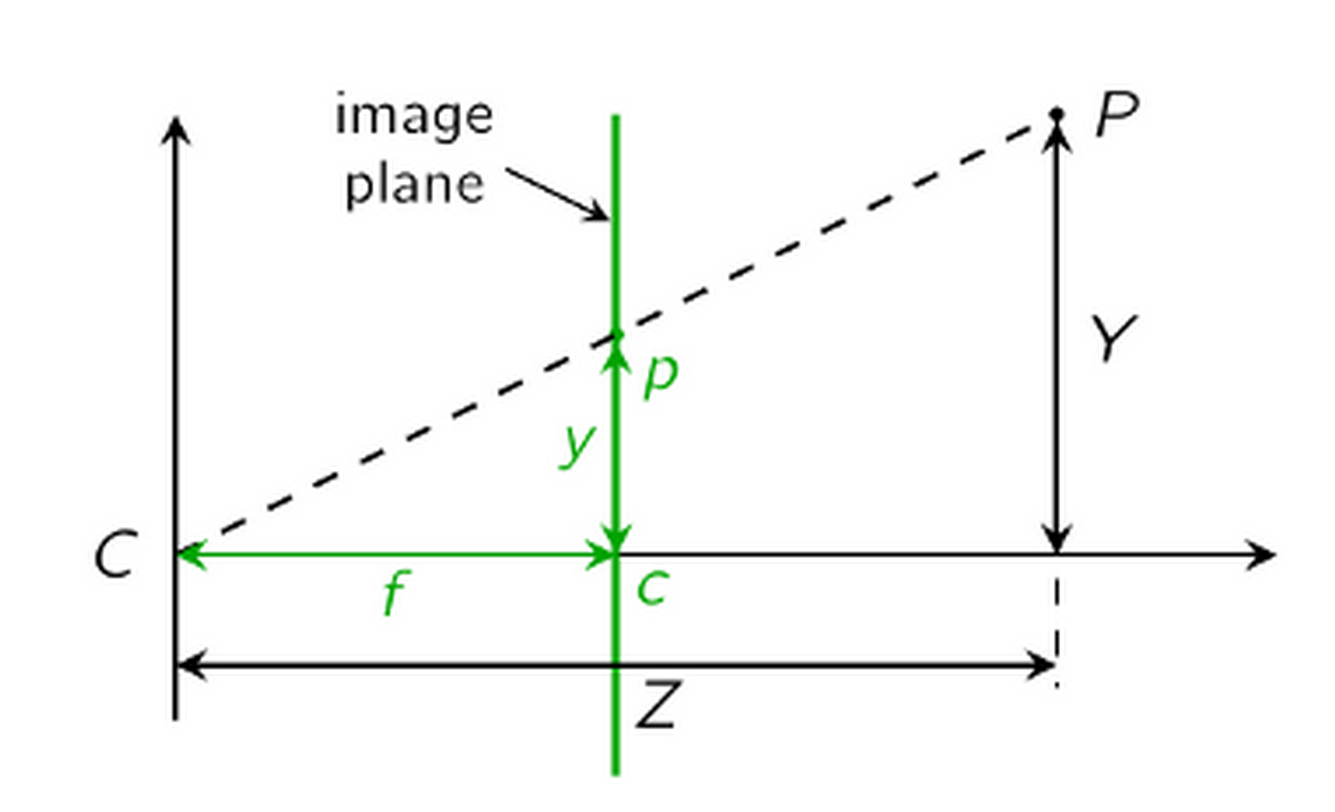
\includegraphics[scale=0.5, angle=0]{Files/Figures/pinhole2.png}
    \caption[Πλάγια όψη του μοντέλου κεντρικής προβολής 2D (pinhole camera model)]{ Πλάγια όψη του μοντέλου κεντρικής προβολής (pinhole camera model) \cite{pinhole} .}
    \label{fig:pinhole2}
\end{figure}

Ως principal point ορίζεται η τομή ανάμεσα στο principal axis και το επίπεδο της εικόνας. Το optical center είναι το σημείο pinhole, το οποίο παίζει κεντρικό ρόλο στην όλη διαδικασία. Η εικόνα μιας pinhole κάμερας σχηματίζεται στο επίπεδο $Z=f$, όπου f είναι το εστιακό μήκος κάμερας(focal length).
Το μοντέλο κάμερας pin-hole χρησιμοποιείται συχνά στην υπολογιστική όραση και τα γραφικά υπολογιστών για την μοντελοποίηση της προβολικής μετατροπής μίας τρισδιάστατης σκηνής σε ένα δισδιάστατο επίπεδο προβολής \cite{hartley2003multiple} .
Το επίπεδο αυτό, που περνάει από το principal point και είναι παράλληλο στο επίπεδο της εικόνα ονομάζεται image plane.
Ό άξονας που ξεκινά από το optical center και το principal point και διαπερνά κάθετα το image plane ονομάζεται principal axis.


Συμπεραίνοντας ότι έχουμε οποιοδήποτε σημείο $\mathbf{P} = \begin{bmatrix}X & Y &Z\end{bmatrix}$ στο 3Δ χώρο, και αν θεωρήσουμε το επίπεδο της εικόνας για να ορίσουμε τη δισδιάστατη εικόνα, η δισδιάστατη προβολή του $\mathbf{P}$ σχηματίζεται στο σημείο τομής ανάμεσα στο επίπεδο της εικόνας και της γραμμής που σχηματίζεται ανάμεσα στο κέντρο της εστίασης και το $\mathbf{p}$, που ορίζεται ως  $\mathbf{p} = \begin{bmatrix}x & y\end{bmatrix}$. 





\subsection{Παράμετροι Κάμερας}

%ksekinoun mathematics
Το μοντέλο της κάμερας έχει στόχο να μετασχηματίσει ένα οποιδήποτε 3D σημείο $\begin{bmatrix} X & Y & Z \end{bmatrix}$ σε ένα 2D σημείο $\begin{bmatrix} x & y\end{bmatrix}$. Για να συμβεί αυτό, αρκεί μία απλή προοπτική προβολή. Χρησιμοποιώντας τη μέθοδο όμοιων τριγώνων στο σχήμα~\ref{fig:pinhole2} παίρνουμε τις παρακάτω σχέσεις:


\begin{equation}
\begin{aligned}
X=f\frac{X}{Z}\\[0.2cm] 
Y=f\frac{Y}{Z}
\end{aligned}
\end{equation}


Η μεταβλητή $f$ συμβολίζει το εστιακό μήκος, ενώ σε μορφή ομογενών συντεταγμένων, η παραπάνω σχέση μπορεί να γραφτεί ως:

\begin{equation}
\begin{bmatrix}
x\\y\\1
\end{bmatrix}
=
\begin{bmatrix}
f & 0 & 0 & 0\\
0 & f & 0 & 0\\
0 & 0 & 1 & 0
\end{bmatrix}
\begin{bmatrix}
X\\
Y\\
Z\\
1
\end{bmatrix}
\end{equation}


Ο παραπάνω πίνακας που ορίζει τη σχέση ανάμεσα στα 3Δ και 2Δ σημεία ονομάζεται και πίνακας προβολής κάμερας (camera projection matrix).




%auto pou pirame einai se metrikes, diladi px metra, kai theloume n to kanoume pixel position



Στη συνέχεια, προκειμένου να μετατρέψουμε τα 2D σημεία αυτά σε pixels πάνω στην εικόνα, πρέπει να χρησιμοποιηθούν ορισμένες παράμετροι της κάμερας που χρησιμοποιείται και ονομάζονται εσωτερικοί παράμετροι κάμερας (intrinsics).
Οι εσωτερικές παράμετροι είναι αυτές που σχετίζονται με την εσωτερική γεωμετρία μίας κάμερας και ορίζουν την αντιστοίχιση των συντεταγμένων στο σύστημα συντεταγμένων της εικόνας (2D) και στο σύστημα συντεταγμένων της κάμερας \cite{Malik2002}. Με άλλα λόγια αναπαριστούν τα οπτικά, γεωμετρικά και ψηφιακα χαρακτηριστικά μιας κάμερας και είναι :

\begin{itemize}
\item Το εστιακό μήκος
\item Η θέση του principal point στο pixel space
\item Ο συντελεστής s σχετικά με το σχήμα των pixels του αισθητήρα
\item οι συντελεστές παραμόρφωσης του φακού
\end{itemize}



Για παράδειγμα, ενώ στο μοντέλο pinhole θεωρήθηκε ότι το σύστημα συντεταγμένων του επιπέδου της εικόνας έχει την αρχή των αξόνων του στο principal point, κάτι τέτοιο μπορεί να μην ισχύει πάντα, ανάλογα με τον αισθητήρα. Έτσι πρέπει να τροποιηθεί το παραπάνω μοντέλο ώστε να ληφθεί υπόψη αυτή η μετατόπιση του συστήματος συντεταγμένων.


\begin{equation}
\begin{aligned}
x_{pix}=x+c_{x}=f\frac{X}{Z}+c_{x}\\[0.3cm]
y_{pix}=y+c_{y}=f\frac{Y}{Z}+c_{y}
\end{aligned}
\end{equation}

όπου $(c_{x},c_{y})^{T}$ είναι οι συντεταγμένες του principal point, δηλαδή του σημείου στο οποίο, ο οπτικός άξονας τέμνει το επίπεδο της εικόνας. 

Οπότε και πάλι σε ομογενείς συντεταγμένες έχουμε τη νέα μορφή:

\begin{equation}
\begin{bmatrix}
x_{pix}\\y_{pix}\\1
\end{bmatrix}
=
\begin{bmatrix}
f & 0 & c_{x} \\
0 & f & c_{y} \\
0 & 0 & 1 
\end{bmatrix}
\begin{bmatrix}
x\\
y\\
1
\end{bmatrix}
=
\begin{bmatrix}
f & 0 & c_{x} & 0\\
0 & f & c_{y} & 0\\
0 & 0 & 1 & 0
\end{bmatrix}
\begin{bmatrix}
X\\
Y\\
Z\\
1
\end{bmatrix}
\end{equation}




Το μοντέλο αυτό, υποθέτει ότι έχουμε τετράγωνα pixels. Αν ωστόσο δε συμβαίνει κάτι τέτοιο, τότε ο μετασχηματισμός από κοσμικές συντεταγμένες σε συντεταγμένες pixel βρίσκεται πολλαπλασιάζοντας την προηγούμενη εξίσωση με το διάνυσμα $\begin{bmatrix}m_{x} & m_{y} & 1\end{bmatrix}$. 
Η αναπαράσταση του μοντέλου της κάμερας γίνεται με ένα πίνακα βαθμονόμησης κάμερας (intrinsic camera calibration matrix) $\mathbf{K}$, ή απλά πίνακα κάμερας (camera matrix).  
Ο πίνακας αυτός γράφεται ως:


\begin{equation}
K=
\begin{bmatrix}
f_{x} & s & c_{x}\\
0 & f_{y} & c_{y}\\
0 & 0 & 1
\end{bmatrix}
\end{equation}

όπου $f_{x}=fm_{x}$ και $f_{y}=fm_{y}$ είναι οι εστιακές αποστάσεις της κάμερας σε όρους διαστάσεων pixels στις κατευθύνσεις x και y αντίστοιχα και $s$ είναι μία παράμετρος λοξότητας (skew) των στοιχείων pixels, η οποία ορίζεται ως η γωνία των δύο πλευρών του κάθε pixel του αισθητήρα και θεωρεί ότι τα pixels δεν είναι πάντα ορθογώνια, αλλά μπορεί να είναι απλά παραλληλόγραμμα. Ωστόσο, με το σημερινό επίπεδο κατασκευής των αισθητήρων, μπορούμε να θεωρήσουμε με ασφάλεια, ότι η παράμετρος αυτή είναι 0, δηλαδή ότι τα pixels του αισθητήρα είναι ορθογώνια, ενώ παράλληλα, στις περισσότερες κάμερες $f_{x}=f_{y}=f$. Τα φυσικά χαρακτηριστικά μιας κάμερας, επομένως, είναι εκείνα που ορίζουν πώς θα διαμορφωθεί μία εικόνα στον αισθητήρα εικόνας μιας κάμερας.

\begin{figure}[H]
    \centering
    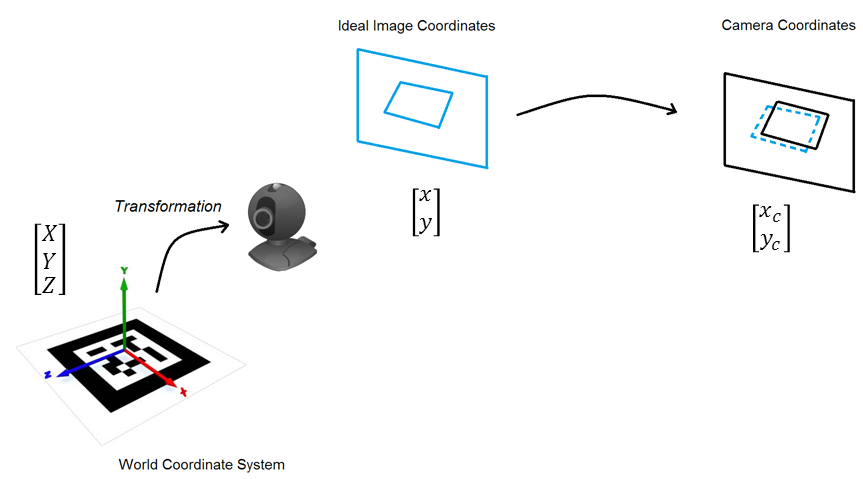
\includegraphics[scale=1.1, angle=0]{Files/Figures/transformation1.png}
    \caption[Μετασχηματισμοί κατά τον εντοπισμό ενός marker]{ Μετασχηματισμοί κατά τον εντοπισμό ενός marker}
    \label{fig:transformation1}
\end{figure}


Mία πραγματική κάμερα μπορεί, επίσης, να παράγει συστηματικά γεωμετρικά σφάλματα, που ονομάζονται παραμορφώσεις, λόγω ατελειών του φακού. 
Επομένως, αυτή η παραμόρφωση πρέπει να ληφθεί υπόψη.


\begin{equation}
D
\left(
\begin{bmatrix}
x_{pix}\\
y_{pix}   
\end{bmatrix}
\right )
=
\begin{bmatrix}
x_{d}\\
y_{d}   
\end{bmatrix}
\end{equation} 



Αυτή η μη-γραμμική παραμόρφωση μπορεί να μοντελοποιηθεί και να εφαρμοστεί όπως στις παρακάτω εξισώσεις. 



\begin{equation}
\begin{cases}x_{d}=x(1+k_{1}r^{2}+k_{2}r^{4}+k_{3}r^{6})+2p_{1}xy+p_{2}(r^{2}+2x^{2})\\
y_{d}=y(1+k_{1}r^{2}+k_{2}r^{4}+k_{3}r^{6})+2p_{2}xy+p_{1}(r^{2}+2y^{2})\end{cases}
\end{equation}

Με τη μοντελοποίηση των παραμορφώσεων αυτών, η αντιστοίχιση που περιγράφεται σε αυτή την ενότητα παίρνει τη μορφή:


\begin{equation}
\begin{bmatrix}
x'_{pix}\\y'_{pix}\\1
\end{bmatrix}
=
\mathbf{K}
\begin{bmatrix}
x_{d}\\
y_{d}\\
1
\end{bmatrix}
\end{equation}








%extrinsics
Οι παραπάνω διαδικασίες υπολογισμού των εσωτερικών παραμέτρων της κάμερας υποθέτουν ότι γνωρίζουμε την 3Δ θέση ενός σημείου ως προς το σύστημα συντεταγμένων της κάμερας. Ωστόσο, η αρχή των αξόνων του συστήματος συντεταγμένων της κάμερας συνήθως διαφέρει από την αρχή των αξόνων του συστήματος συντεταγμένων κόσμου.
Αν θέλουμε να βρούμε την προβολή του σημείου το οποίο ορίζεται ως προς ένα αυθαίρετο σύστημα συντεταγμένων, τότε πρέπει να βρούμε τις εξωτερικές παραμέτρους που ορίζουν το μετασχηματισμό. Οι εξωτερικές παράμετροι(extrinsics) ορίζουν τη θέση και το προσανατολισμό της κάμερας ( ή ακριβέστερα του συστήματος συντεταγμένων της κάμερας σε σχέση με τις κοσμικές συντεταγμένες της σκηνής). 

Έχουμε επομένως 2 συστήματα συντεταγμένων:

\begin{itemize}
\item Το σύστημα συντεταγμένων της κάμερας 
\item Το σύστημα συντεταγμένων του κόσμου (world coordinates system)
\end{itemize}



Ο μετασχηματισμός αυτός ορίζεται με τη μορφή ενός πίνακα διαστάσεων 3x4 $\mathbf{T}=\begin{bmatrix}\mathbf{R} & | & \!\mathbf{t}\end{bmatrix}$, ή σε ομογενείς συντεταγμένες :

\begin{equation}
\begin{bmatrix}
X_{cam} \\ Y_{cam} \\ Z_{cam}
\end{bmatrix}
=
\begin{bmatrix}
r_{1} & r_{2} & r_{3} & t_{x}\\
r_{4} & r_{5} & r_{6} & t_{y}\\
r_{7} & r_{8} & r_{9} & t_{z}
\end{bmatrix}
\begin{bmatrix}
X_{world}\\
Y_{world}\\
Z_{world}\\
1
\end{bmatrix}
=\mathbf{T}\begin{bmatrix}
X_{world}\\
Y_{world}\\
Z_{world}\\
1
\end{bmatrix}
\end{equation}

Όπως είναι γνωστό, ένας πίνακας περιστροφής έχει μόνο τρεις παραμέτρους $(\alpha, \beta, \gamma)$ και αναφέρονται στην περιστροφή ως προς τους 3 άξονες, οι οποίες ορίζουν τα 9 στοιχεία του. Ένα διάνυσμα μετατόπισης έχει επίσης 3 παραμέτρους και επομένως ο πίνακας πόζας έχει συνολικά $3+3=6$ ελεύθερες παραμέτρους. Όπως μπορεί να γίνει εύκολα αντιληπτό, ο συνδυασμός μετατόπισης και περιστροφής μπορεί να μοντελοποιήσει οποιαδήποτε κίνηση της κάμερας. Ένα σύστημα εντοπισμού marker πρέπει να λύνει αυτό τον πίνακα σε κάθε frame, όταν ανιχνεύει έναν marker.





%---------------------------------------------%

\subsection{Βαθμονόμηση Κάμερας}
%Η ΔΙΑΔΙΚΑΣΙΑ ΒΑΘΜΟΝΟΜΗΣΗΣ ΚΑΙ ΓΕΝΙΚΑ Η ΘΕΩΡΙΑ ΑΠΟ ΠΙΣΩ(ΤΟ ΠΩς ΓΙΝΕΤΑΙ ΣΤΟ ΚΕΦΑΛΑΙΟ 4)


Η διαδικασία υπολογισμού των εσωτερικών παραμέτρων της κάμερας ονομάζεται βαθμονόμηση κάμερας ή camera calibration. 
Η διαδικασία της βαθμονόμησης περιλαμβάνει, ουσιαστικά, την ταυτοποίηση των εσωτερικών παραμέτρων της κάμερας, δηλαδή του πίνακα κάμερας και την εκτίμηση των συντελεστών παραμόρφωσης $(k1, k2, p1, p2, k3)$.

Η συνολική απόδοση μιας εφαρμογής επαυξημένης πραγματικότητας, εξαρτάται άμεσα από την ακρίβεια της βαθμονόμησης της κάμερας. Παρά το γεγονός ότι το αντικείμενο παρουσιάζει ιδιαίτερο ερευνητικό ενδιαφέρον, δεν είναι στους στόχους της εργασίας η περαιτέρω ανάλυσή του.  
Καθώς οι παράμετροι εξαρτώνται μόνο από την ίδια την κάμερα ( και όχι από τη θέση και τον προσανατολισμό της), η διαδικασία της βαθμονόμησης, οι εφαρμογές επαυξημένης πραγματικότητας συχνά χρησιμοποιούν ξεχωριστά εργαλεία βαθμονόμησης ή διενεργούν την διαδικασία βαθμονόμησης ξεχωριστά από την εφαρμογή. 


Στα πλαίσια της διπλωματικής εργασίας απαιτείται η χρήση μιας απλής μεθόδου με αξιοποίηση συνηθισμένου εξοπλισμού για την βαθμονόμηση. Η διαδικασία της βαθμονόμησης απλοποιείται χρησιμοποιώντας ένα υπολογιστικό εργαλείο της OpenCV. Η διαδικασία περιλαμβάνει την καταγραφή ενός συνόλου φωτογραφιών ενός calibration board, και ο αλγόριθμος του εργαλείου υπολογίζει τις εσωτερικές παραμέτρους.
Το εργαλείο βαθμονόμησης αποθηκεύει τα αποτελέσματα σε ένα αρχείο, το οποίο διαβάζει η εφαρμογή επαυξημένης πραγματικότητας στην αρχή της εκτέλεσής της. Από εδώ και στο εξής θα θεωρούμε ότι η συνάρτηση αντίστροφης παραμόρφωσης (undistortion) $D^{-1}$ και ο πίνακας βαθμονόμησης Κ γίνονται γνωστά, μόλις γίνει η βαθμονόμηση μιας κάμερας.



%σκακιερα
Καταφεύγουμε λοιπόν, στη λύση του εργαλείου της Opencv για την βαθμονόμηση της κάμερας\cite{calibrationtool}, που προσφέρει μία έτοιμη και αποτελεσματική λύση, με χρήση μίας απλής κάμερας και μιας απλής επίπεδης εικόνας και συγκεκριμένα του μοτίβου τετραγώνων σκακιέρας, η οποία χρειάζεται απλά να εκτυπωθεί σε απλό χαρτί. 
Γενικά, η βαθμονόμηση μέσω της καταγραφής πολλαπλών λήψεων ενός επίπεδου αντικειμένου με χαρακτηριστικά σημεία, όπως είναι η σκακιέρα, επιτυγχάνεται με δεδομένα τις συντεταγμένες χώρου και εικόνας των αντίστοιχων σημείων, οι πρώτες εκ των οποίων προκύπτουν αυτόματα, ενώ οι τελευταίες αναγνωρίζονται στην εικόνα ομοίως με αυτόματο τρόπο. Ωστόσο, για την εξασφάλιση σωστών αποτελεσμάτων από τη διαδικασία της βαθμονόμησης, οι εικόνες του αντικειμένου πρέπει να ληφθούν από διαφορετικά σημεία και υπό διαφορετικές γωνίες. 


Αυτό το οποίο θα πρέπει να συγκρατήσει ο αναγνώστης, είναι ότι μέσω της διαδικασίας της βαθμονόμησης παίρνουμε τις εσωτερικές παραμέτρους της κάμερας μέσω μιας offline διαδικασίας που πραγματοποιείται μόνο μία φορά στην αρχή της διαδικασίας ανάπτυξης της εφαρμογής. Οι παράμετροι που υπολογίζονται, ορίζονται ως είσοδος στην εφαρμογή που θα αναπτυχθεί, προκειμένου να λειτουργήσει σωστά. Επομένως, δε χρειάζεται να πραγματοποιείται βαθμονόμηση κάθε φορά πριν ξεκινήσει μία εφαρμογή επαυξημένης πραγματικότητας. Αρκεί να γίνει μόνο μία φορά στην αρχή, εκτός και αν τα αποτελέσματα δεν έχουν αρκετή ακρίβεια. Ωστόσο αν σε ένα σύστημα επαυξημένης πραγματικότητας χρησιμοποιηθεί διαφορετική κάμερα, τότε πρέπει να γίνει εκ νέου βαθμονόμηση για τη νέα κάμερα.







\subsection{Εκτίμηση Θέσης Marker}

Ένα σύστημα εντοπισμού marker μπορεί να μετατρέψει τις συντεταγμένες εικόνας που παρατηρείται στην οθόνη (pixel coordinates) μιας βαθμονομημένης κάμερας σε ιδανικές συντεταγμένες συντεταγμένες εικόνας. 
Για να πάρουμε επομένως τον κατάλληλο πίνακα προβολής, για μία αυθαίρετη θέση της κάμερας στο χώρο, πρέπει να υπολογιστούν ανεξάρτητα οι εσωτερικές και οι εξωτερικές παράμετροι της κάμερας. 



Η παρακάτω εξίσωση δείχνει το πλήρες μοντέλο προοπτικής που χρησιμοποιείται κατά τη διαδικασία.


\begin{equation} 
\begin{split}
P
&=
\overbrace{
\mathbf{K}}^\text{Intrinsic Matrix} \times 
\overbrace{
\mathbf{T}
}^\text{Extrinsic Matrix} 
\\&=
\overbrace{
\begin{bmatrix}
1 & 0 & c_{x} \\ 
0 & 1 & c_{y} \\ 
0 & 0 & 1  
\end{bmatrix}
\times 
\begin{bmatrix}
f_{x} & 0 & 0 \\ 
0 & f_{y} & 0 \\ 
0 & 0 & 1  
\end{bmatrix}
\times
\begin{bmatrix}
1 & s/f_{x} & 0 \\ 
0 & 1 & 0 \\ 
0 & 0 & 1  
\end{bmatrix}
}^\text{Intrinsic Matrix}
\times
\overbrace{
\begin{bmatrix}
&\mathbf{I}& |& \mathbf{t}&
\end{bmatrix}
\times
\begin{bmatrix}
\mathbf{R} &    0 \\
0 &    1 
\end{bmatrix}}^\text{Extrinsic Matrix}
\end{split}
\end{equation}


Για να μπορέσει μία εφαρμογή επαυξημένης πραγματικότητας να απεικονίσει σωστά ένα εικονικό τρισδιάστατο αντικείμενο πάνω από μία πραγματική σκηνή, οι παραπάνω γεωμετρικοί μετασχηματισμοί πρέπει να είναι ακριβείς. H σημασία τους στην επαυξημένη πραγματικότητα είναι τεράστια. Ένα σφάλμα σε οποιαδήποτε από τις σχέσεις θα κάνει ανακριβές το registration, ελαττώνοντας το ρεαλισμό της τελικής επαυξημένης σκηνής. 


Η εύρεση των εξωτερικών παραμέτρων ( με δεδομένη την εκ των προτέρων γνώση των εσωτερικών παραμέτρων) δίνει τη θέση και τον προσανατολισμό της κάμερας σε σχέση με τον πραγματικό δισδιάστατο κόσμο είναι γνωστή σαν εκτίμηση πόζας (pose estimation).



\begin{figure}[H]
    \centering
    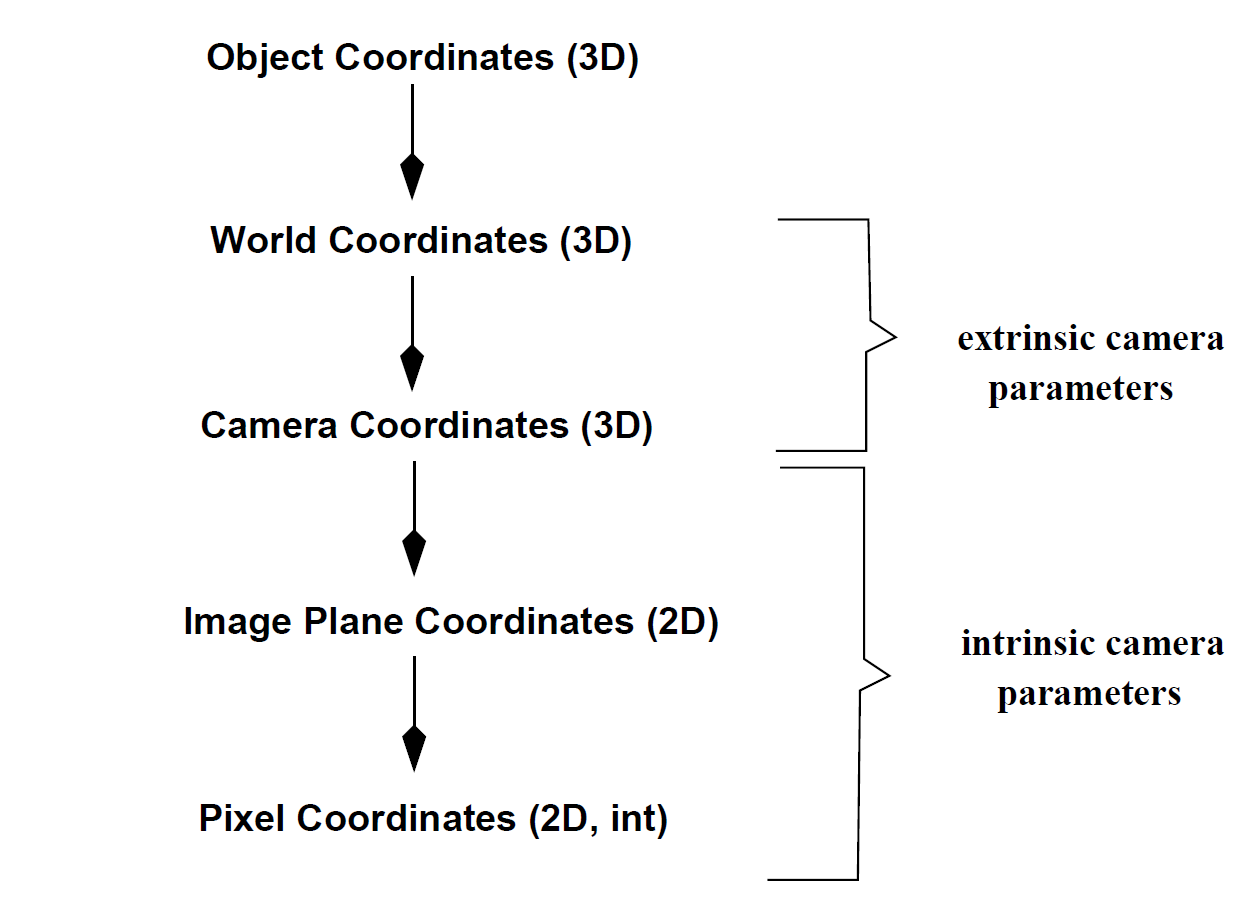
\includegraphics[scale=0.7, angle=0]{Files/Figures/coordinatesDiagram.png}
    \caption[Σειρά μετασχηματισμών]{ Σειρά μετασχηματισμών}
    \label{fig:coordinatesDiagram}
\end{figure}


\subsection{Ανίχνευση Marker}




%siltanen
Ένας καλός marker πρέπει να μπορεί να ανιχνευθεί εύκολα και αξιόπιστα κάτω από οποιοεσδήποτε συνθήκες. 
Ορισμένες διαφορές στην φωτεινότητα(luminance) εντοπίζονται ευκολότερα από διαφορές στο χρώμα (colour) αν χρησιμοποιηθούν τεχνικές όρασης υπολογιστών \cite{hartley2003multiple} . 
Επιπλέον, ο φωτισμός αλλάζει τα αντιληφθέντα χρώματα των αντικειμένων και επομένως η ανίχνευση χρώματος είναι δύσκολη. 
Φυσικά, όσο περισσότερη αντίθεση φωτισμού υπάρχει, τόσο ευκολότερα εντοπίζονται αντικείμενα. 


Υπό αυτή την έννοια, η χρήση ασπρόμαυρων markers βελτιστοποιεί την διαδικασία ανίχνευσης. Το σύστημα πρέπει επίσης να μπορεί να υπολογίζει την πόζα της κάμερας με βάση το marker που εντοπίστηκε. Για να συμβεί αυτό, αρκεί να εντοπιστούν 4 σημεία στην εικόνα και έτσι μπορούμε να υπολογίσουμε την μία και μοναδική λύση για την πόζα της κάμερας και ο ευκολότερος τρόπος για να συμβεί αυτό είναι η χρήση του σχήματος τετραγώνου για τα markers. 
Επιπλέον, οι θέσεις των γωνιακών σημείων είναι γενικά εύκολο να υπολογιστούν, καθώς αποτελούν ουσιαστικά την τομή των ακραίων ακμών ενός marker. Συμπερασματικά, τα περισσότερα συστήματα χρησιμοποιούν ασπρόμαυρους δείκτες και για αυτό το λόγο θα επεξηγηθεί στη συνέχεια η διαδικασία ανίχνευσης ασπρόμαυρων markers σε μία εικόνα.    




Ο πρωταρχικός στόχος μιας διαδικασίας ανίχνευσης marker είναι η εύρεση των περιγραμμάτων πιθανών markers και μετέπειτα η εξαγωγή των γωνιών τους στην εικόνα. Επιπλέον, το σύστημα ανίχνευσης πρέπει να εξακριβώσει ότι αυτό που βρέθηκε είναι όντως marker και να αποκωδικοποιήσει την ταυτότητα του. 
Τέλος το σύστημα υπολογίζει την πόζα, με βάση τις πληροφορίες από τη θέση στην οποία ανιχνεύθηκε ο marker.

Τα βασικά βήματα ανίχνευσης είναι τα παρακάτω:


\begin{description}

\item[Ανάκτηση εικόνας]
Ανάκτηση μίας εικόνας έντασης επιπέδων του γκρι.
Το στάδιο της απόκτησης εικόνας είναι ουσιαστικά μια ξεχωριστή διαδικασία. Πριν από την πραγματική ανίχνευση ενός marker, το σύστημα πρέπει να πάρει μία εικόνας έντασης (greyscale image) για να ξεκινήσει η διαδικασία ανίχνευσης. Aν το format της εικόνας που καταγράφηκε είναι άλλου τύπου, πχ RGB, τότε θα μετασχηματιστεί σε εικόνας κλίμακας γκρι χρησιμοποιώντας μία γνωστές τεχνικές \cite{Gonzalez}. 


\item[Προεπεξεργασία] Αφού γίνει αντιστροφή της παραμόρφωσης λόγω του φακού της κάμερας, πρώτος στόχος είναι η ανίχνευση των ακμών πιθανών markers. 
Συνήθως, είτε γίνεται πρώτα κατωφλίωση της εικόνας και έπειτα αναζήτηση για markers από τη δυαδική εικόνα που προκύπτει, είτε γίνεται ανίχνευση ακμών από την εικόνα κλίμακας του γκρι. Αυτές οι μέθοδοι επεξεργασίας χαμηλού επιπέδου(thresholding,
edge detection, line fitting, etc.) είναι γνωστές \cite{Gonzalez}, \cite{szeliski2010computer} και επομένως δε θα αναλυθούν περαιτέρω στη συγκεκριμένα εργασία. 


Τα συστήματα τα οποία χρησιμοποιούν προσεγγίσεις κατωφλίωσης, συνήθως χρησιμοποιούν μεθόδους προσαρμοστικής κατωφλίωσης ώστε να αντιμετωπίσουν τις τοπικές αλλαγές φωτεινότητας. 
Μετά την κατωφλίωση το σύστημα έχει μία δυαδική εικόνα που αποτελείται από το παρασκήνιο και τα αντικείμενα. Όλα τα αντικείμενα είναι πιθανοί υποψήφιοι markers σε αυτό το στάδιο.
Συνήθως η επόμενη φάση είναι η επισήμανσή τους ή ο συνεχής εντοπισμός τους. \\
Κατά τη διαδικασία της επισήμανσης το σύστημα μπορεί να απορρίψει αντικείμενα τα οποία είτε είναι πολύ μικρά είτε είναι οτιδήποτε άλλο εκτός από marker. Τέλος οι ακμές όλων των πιθανών markers επισημαίνονται και οι θέσεις τους εξομαλύνονται(undistort) για το στάδιο του line fitting. 
Έπειτα, το σύστημα εξετάζει και πάλι πιθανά markers, ελέγχοντας αν έχουν 4 ευθείες γραμμές και 4 γωνίες. Τέλος, το σύστημα βελτιστοποιεί τις θέσεις των γωνιών με ακρίβει sub-pixel. 
Η ανίχνευση ακμών σε εικόνες κλίμακας του γκρι είναι μία διαδικασία που παίρνει αρκετό χρόνο και επομένως τα συστήματα συνήθως χρησιμοποιούν υποδειγματοληψία και ανιχνεύουν ακμές μόνο σε ένα προκαθορισμένο πλέγμα.
Συνήθως οι εικόνες δεν είναι παραμορφωμένες, αφού χρησιμοποιείται η αντίστροφη διαδικασία παραμόρφωσης η οποία υπολογίστηκε κατά τη διαδικασία της βαθμονόμησης. Ωστόσο στα συστήματα πραγματικού χρόνου, εξομαλύνονται μόνο οι θέσεις των σημείων χαρακτηριστικών, π.χ οι ακμές ενός marker που ανιχνεύθηκαν για να επιταχυνθεί η διαδικασία. 

Ακόμα και μικρά λάθη σε εντοπισμένες δισδιάστατες θέσεις ακμών και γωνιών επηρεάζουν την πόζα της κάμερας όταν υπολογίζεται. Λάθη ανίχνευσης μπορεί να συμβούν λόγω σφάλματος κβαντοποίησης pixel, λαθασμένης τιμής ορίου κατωφλίωσης, θολώματος κίνησης, θορύβου κλπ. Αυτά τα σφάλματα προκαλούν ενοχλητικό τρέμουλο (jitter) στην πόζα ενός αντικειμένου, ακόμα και αν η κάμερα κινείται ελάχιστα. 
Για να βελτιωθεί η ακρίβεια, τα συστήματα βελτιστοποιούν τις θέσεις μετά την αρχική ανίχνευση.


\item[Ανίχνευση πιθανών markers και απόρριψη non-markers ] Οι εφαρμογές επαυξημένης πραγματικότητας στοχεύουν σε επεξεργασία πραγματικού χρόνου και γρήγορες αποδόσεις, καθώς αυτές θεωρούνται επιτακτικές. Τα συστήματα δεν μπορούν να σπαταλήσουν πολύτιμο χρόνο υπολογισμών στην επεξεργασία στοιχείων που δεν είναι markers. Επομένως, πολλές υλοποιήσεις χρησιμοποιούν κριτήρια αποδοχής / απόρριψης για να ξεχωρίσουν τα πραγματικά markers από τα αντικείμενα που προφανώς είναι οτιδήποτε άλλο.Στη συνέχεια αναλύουμε ορισμένα τέτοια τεστ που χρησιμοποιούνται συχνά.


Ένα σύστημα μπορεί να απορρίψει περιοχές που αποτελούνται μόνο από μερικά pixels. Συνήθως οι περιοχές αυτές δεν είναι markers, αλλά και να ήταν, το μικρό μέγεθός τους θα σήμαινε ότι το marker είναι πολύ μακριά από την κάμερα. Σε αυτή την περίπτωση η πόζα του marker δε θα ήταν πολύ ακριβής και απομένως άχρηστη. Επιπλέον, αν το marker συρρικνωθεί σε μέγεθος μερικών μόνο pixels, το σύστημα δε θα μπορεί να το αναγνωρίσει, εκτός αν κρατά ιστορικό εμφάνισης κάθε marker.


Το σύστημα πρέπει να δίνει προσοχή σε περιοχές στο εσωτερικό των markers και να σιγουρευτεί ότι δεν αφαιρεί κομμάτια ή στοιχεία που ανήκουν στο marker. Το ιστόγραμμα ενός ασπρόμαυρου marker είναι διπολικό και το σύστημα μπορεί να αξιοποιήσει τη διπολικότητα αυτή ως ένα κριτήριο για γρήγορη αποδοχή ή απόρριψη. Ωστόσο, το τεστ πρέπει να λάβει υπόψη του τις αντανακλάσεις, οι οποίες μπορεί να δημιουργήσουν τιμές στη μέση του ιστογράμματος (γκρι περιοχές). 


Ο υπολογισμός του αριθμού των εικονοστοιχείων που ανήκουν στην περίμετρο είναι μία γρήγορη διαδικασία η οποία μπορεί να πραγματοποιηθεί στο στάδιο της επισήμανσης, σε αντίθεση με τον υπολογισμό του μεγέθους του αντικειμένου που είναι πιο περίπλοκο και απαιτεί χρόνο. Ένα άλλο γρήγορο κριτήριο που χρησιμοποιείται για την εκτίμηση της περιοχής, είναι η μέγιστη διαγώνιος ή άνοιγμα. Μερικές φορές ένα σύστημα μπορεί να απορρίψει περιοχές που είναι πολύ μεγάλες αν έχει γνώση για να δικαιολογήσει το συμπέρασμα ότι είναι κάτι άλλο εκτός από marker.


Το βέλτιστο όριο για το μέγεθος ενός marker εξαρτάται από την εφαρμογή και τον τύπο του marker. Για παράδειγμα, το ARToolKit συμπεραίνει ότι τα markers είναι σε μία λογική απόσταση από την κάμερα. Η ανίχνευση markers του ARToolKit παραβλέπει περιοχές που είναι πολύ μεγάλες ή πολύ μικρές μετά την επισήμανση. Με άλλα λόγια, κρατά τις περιοχές όπου ο αριθμός των pixels που ανήκουν σε αυτές είναι μέσα στα όρια για περαιτέρω ανάλυση.


Ανάλογα με τον τύπο του marker, ένα σύστημα μπορεί να γνωρίζει κάτι για την συνολική εμφάνιση του marker. Για παράδειγμα, τα απλά πρότυπα markers έχουν μία μαύρη εκόνα σε μία λευκή περιοχή που περιβάλλεται από μία μαύρη ακμή.
Σε μία ιδεατή περίπτωση, οι markers έχουν ένα γνωστό αριθμό από οπές (λευκές περιοχές) μέσα σε μία μαύρη περιοχή του marker. Επιπλέον οι περιοχές που είναι εντελώς μαύρες, δεν είναι markers σίγουρα. Ο υπολογισμός του αριθμού των οπών είναι γρήγορος και επομένως ένα σύστημα μπορεί να εφαρμόσει σαν κριτήριο απόρριψης τον αριθμό των οπών, κατά την προεπεξεργασία.


Μια ευρετική μέθοδος απόρριψης προφανών μη-markers είναι ο υπολογισμός αριθμού αλλαγών έντασης σε δύο κάθετες κατευθύνσεις. Αν ο αριθμός αλλαγών είναι χαμηλός, τότε δεν μπορεί να είναι marker. Αυτό το κριτήριο λειτουργεί μόνο σε τύπους markers όπου η κωδικοποίηση εγγυάται υψηλή διακύμανση και μη ύπαρξη σχεδόν λευκών ή σχεδόν μαύρων markers. 


Μία προοπτική εικόνα ενός τετραγώνου είναι πάντα τετράπλευρη. Επομένως, βολεύει να εφαρμοστεί ένα τεστ τετραπλεύρων για τετράγωνα markers. Ο αριθμός γραμμών και γωνιών είναι εύκολο να υπολογίστει και επομένως οι υλοποιήσεις ανίχνευσης markers χρησιμοποιούν το συγκεκριμένο κριτήριο.Για παράδειγμα το ARToolKit χρησιμοποιεί line fitting για τα pixels των ακμών για να ελέγξει την ύπαρξη ακριβώς 4 γραμμών στην περίμετρο.


Στην επεξεργασία πραγματικού χρόνου, το σύστημα πρέπει να επικεντρώνεται στην επεξεργασία σχετικών πληροφοριών και επομένως αυτά τα γρήγορα τεστ είναι ιδιαίτερα σημαντικά. Τα τεστ αυτά πραγματοποιούνται από τα συστήματα καθόλη τη διάρκεια της ανίχνευσης markers και της διαδικασίας ταυτοποίησης. 


\item [Aποκωδικοποίηση markers] Στο στάδιο αυτό, πρέπει να πάρουμε μία εμπροσθια όψη του marker χρησιμοποιώντας τις αρχές της ομογραφίας (homography) και να αντιστοιχίσουμε τον κωδικό με μία δομή που περιγράφει το αντικείμενο το οποίο αντιστοιχεί στο marker.


\item Υπολογισμός πόζας marker Το στάδιο αυτό αναλύθηκε στην προηγούμενη ενότητα. Ουσιαστικά γίνεται εκτίμηση της θέσης του marker ως προς την κάμερα, καθώς επίσης πραγματοποιείται επαναληπτικός υπολογισμός της πόζας του για μεγαλύτερη ακρίβεια.


\end{description}



Γενικά οι διαδικασίες ανίχνευσης marker μπορούν να διαφέρουν από την παραπάνω σειρά βημάτων. Μπορεί η σειρά εκτέλεσης να είναι διαφορετική ή το σύστημα να συνενώσει βήματα στον ίδιο αλγόριθμο. Συγκεκριμένα, πολλές υλοποιήσεις συνδυάζουν τεστ αποδοχής/απόρριψης με άλλες διεργασίες. Το σύστημα μπορεί να απορρίψει ένα υποψήφιο marker σε οποιοδήποτε στάδιο της ανίχνευσης, μόλις παρατηρήσει ότι ο υποψήφιος δεν μπορεί να είναι marker. Ωστόσο η βασική αρχή είναι η ίδια συνήθως. 




%aruco
Στην διπλωματική αυτή εργασία, χρησιμοποιήθηκε η βιβλιοθήκη επαυξημένης πραγματικότητας ArUco. Η διαδικασία που χρησιμοποιείται για την ανίχνευση ενός marker κρίνεται σκόπιμο να αναλυθεί στη συνέχεια.



\begin{itemize}
\item Αρχικά εφαρμόζεται αλγόριθμος προσαρμοστικής κατωφλίωσης για την λήψη των ακμών σχημάτων (Figure 1)

\begin{figure}[H]
    \centering
    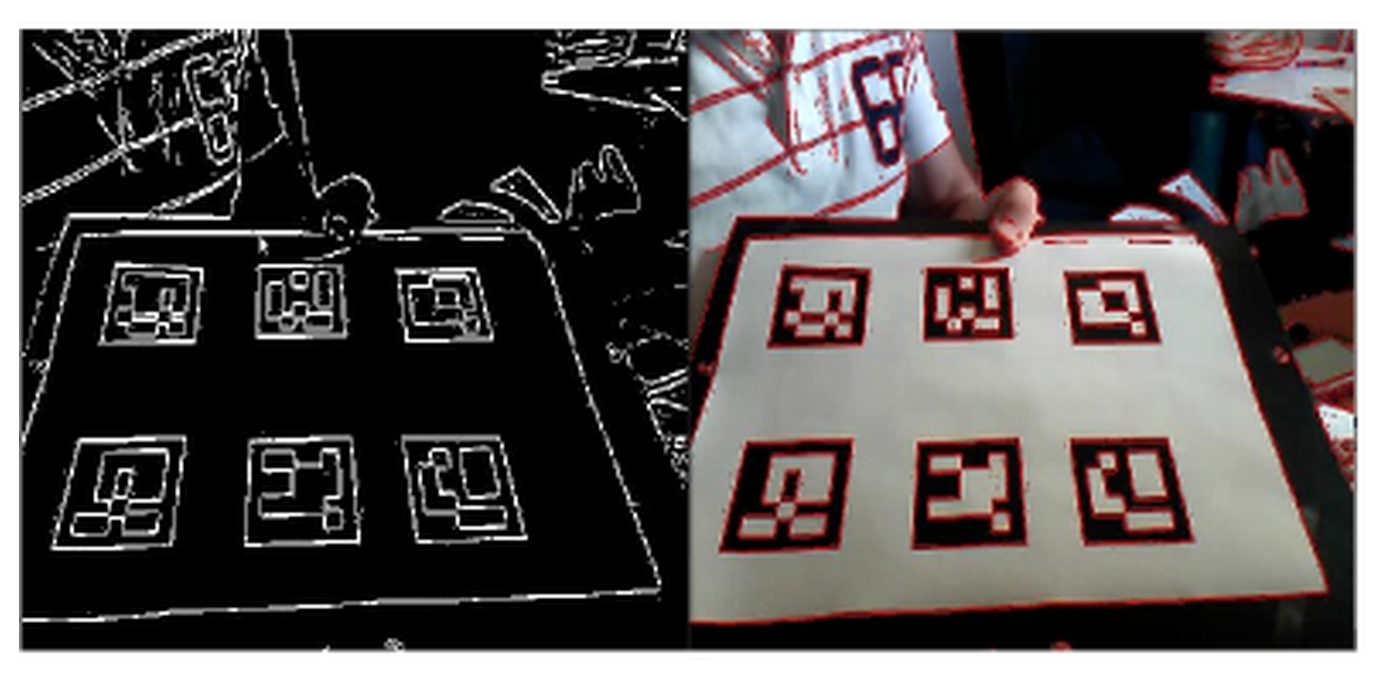
\includegraphics[scale=0.6, angle=0]{Files/Figures/aruco1.png}
    \caption[Παράδειγμα εντοπισμού marker και επαύξησης της σκηνής \cite{howmarkerswork}]{ Παράδειγμα εντοπισμού marker και επαύξησης της σκηνής }
    \label{fig:aruco1}
\end{figure}


\item  Στη συνέχεια γίνεται εντοπισμός των περιγραμμάτων της εικόνας.Βέβαια, έτσι ανιχνεύονται όχι μόνο τα πραγματικά markers, αλλά και πολλά σύνορα σχημάτων που δε χρειάζονται. Για το λόγο αυτό, χρειάζεται να φιλτραριστούν τα εικονοστοιχεία των συνόρων που δεν χρειάζονται. 

Επομένως, αρχικά αφαιρούνται τα σύνορα που έχουν μικρό αριθμό σημείων.


\begin{figure}[H]
    \centering
    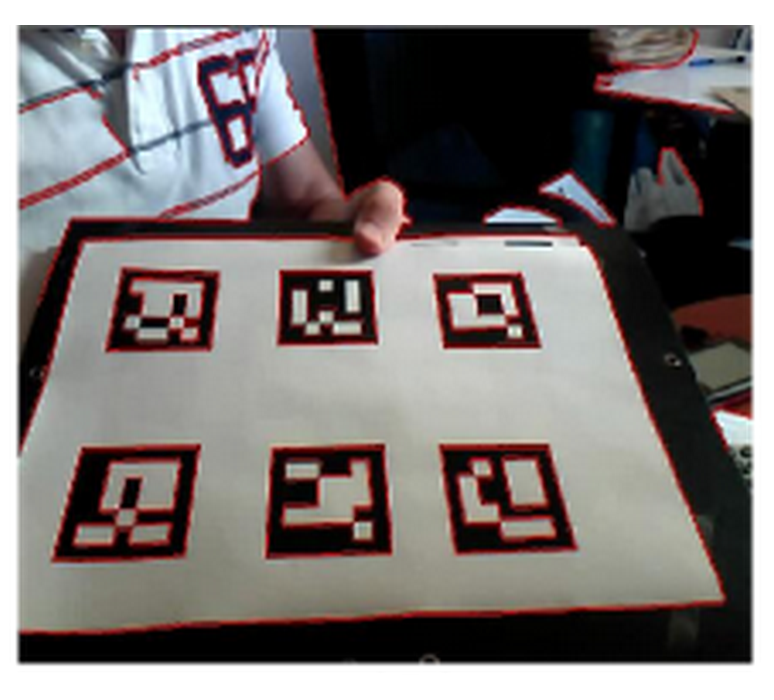
\includegraphics[scale=0.6, angle=0]{Files/Figures/aruco2.png}
    \caption[Παράδειγμα εντοπισμού marker και επαύξησης της σκηνής \cite{howmarkerswork}]{ Παράδειγμα εντοπισμού marker και επαύξησης της σκηνής \cite{howmarkerswork}}
    \label{fig:aruco2}
\end{figure}



Μετέπειτα, πραγματοποιείται πολυγωνική προσέγγιση των περιγραμμάτων και διατηρούνται τα κοίλα περιγράμματα 4 γωνιών (π.χ τετραγώνων). 


\begin{figure}[H]
    \centering
    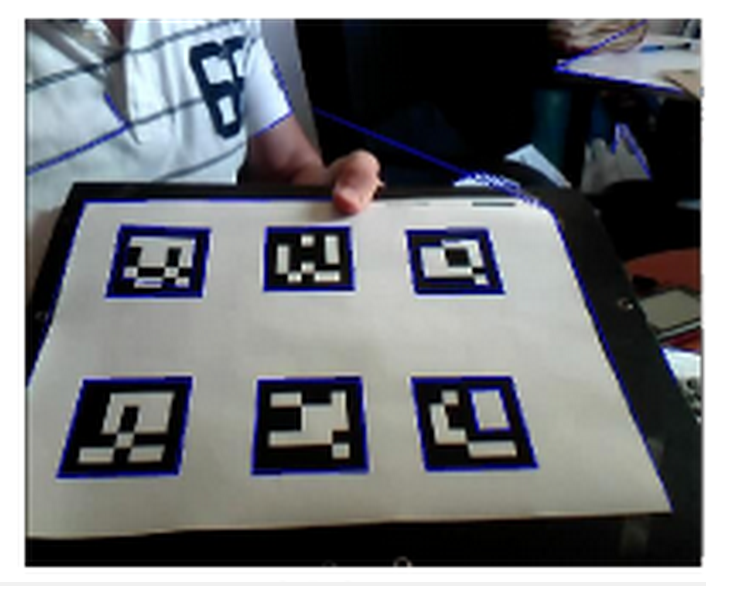
\includegraphics[scale=0.6, angle=0]{Files/Figures/aruco3.png}
    \caption[Παράδειγμα εντοπισμού marker και επαύξησης της σκηνής \cite{howmarkerswork}]{ Παράδειγμα εντοπισμού marker και επαύξησης της σκηνής \cite{howmarkerswork}}
    \label{fig:aruco3}
\end{figure}



\item Ταξινόμηση των γωνιών με φορά ανίθετης της κατεύθυνσης του ρολογιού.


\item Αφαίρεση των ορθογωνίων που βρίσκονται πολύ κοντά το ένα με το άλλο. Αυτό απαιτείται διότι η προσαρμοστική κατωφλίωση συνήθως ανιχνεύει το εξωτερικό μέρος του συνόρου ενός marker. Σε αυτό το στάδιο κρατάμε το σύνορο που βρίσκεται πιο έξω.


\begin{figure}[H]
    \centering
    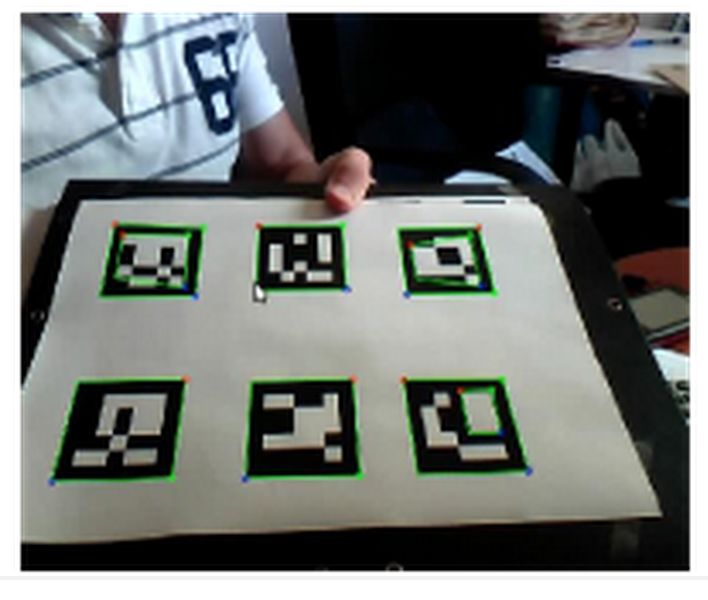
\includegraphics[scale=0.6, angle=0]{Files/Figures/aruco4.png}
    \caption[Παράδειγμα εντοπισμού marker και επαύξησης της σκηνής \cite{howmarkerswork}]{ Παράδειγμα εντοπισμού marker και επαύξησης της σκηνής \cite{howmarkerswork}}
    \label{fig:aruco4}
\end{figure}




\item Ταυτοποίηση Marker (Marker Identification)



\begin{itemize}


\item Κατά τη διαδικασία της ταυτοποίησης, πραγματοποιείται αφαίρεση της προοπτικής προβολής ώστε να πάρουμε μία εμπροσθια όψη της τετραγωνικής περιοχής χρησιμοποιώντας τις αρχές της ομογραφίας (homography).


\begin{figure}[H]
    \centering
    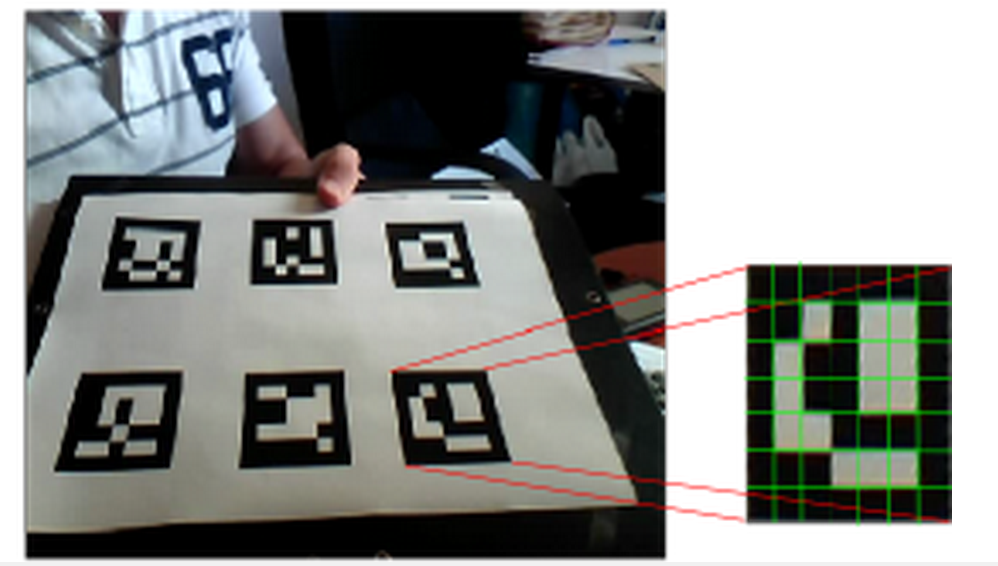
\includegraphics[scale=0.6, angle=0]{Files/Figures/aruco5.png}
    \caption[Παράδειγμα εντοπισμού marker και επαύξησης της σκηνής \cite{howmarkerswork}]{ Παράδειγμα εντοπισμού marker και επαύξησης της σκηνής \cite{howmarkerswork}}
    \label{fig:aruco5}
\end{figure}



\item Πραγματοποιείται κατωφλίωση της εικόνας χρησιμοποιώντας τη μέθοδο Otsu. Η μέθοδος αυτή είναι μια μη παραμετρική μέθοδος κατωφλίωσης η οποία βασίζεται στο ιστόγραμμα της εικόνας. Πιο συγκεκριμένα βρίσκει εκείνο το κατώτατο όριο το οποίο ελαχιστοποιεί τη διακύμανση κάθε κλάσης των οριοθετημένων μαύρων και άσπρων pixels. Με άλλα λόγια η προσέγγιση αυτή επιλέγει το κατώφλι το οποίο έχει ως αποτέλεσμα την πιο σφιχτή ομαδοποίηση των δύο ομάδων που αναπαρίστανται από τα pixels παρασκηνίου και προσκηνίου. 


\item Ταυτοποίηση του εσωτερικού κωδικού. Το marker υποδιαιρείται σε ένα πλέγμα 6x6, όπου τα εσωτερικά 5x5 κελιά περιέχουν την πληροφορία για το ID του marker. Τα υπόλοιπα αντιστοιχούν σε ένα εξωτερικό μαύρο σύνορο. Η βιβλιοθήκη της ArUco ελέγχει πρώτα αν το εξωτερικό μαύρο σύνορο υπάρχει. Έπειτα, γίνεται ανάγνωση των εσωτερικών 5x5 κελιών και έλεγχος σχετικά με το αν παρέχουν έναν έγκυρο κωδικό (ίσως χρειαστεί η περιστροφή του κωδικού για να πάρουμε έγκυρο κωδικό). 



\begin{figure}[H]
    \centering
    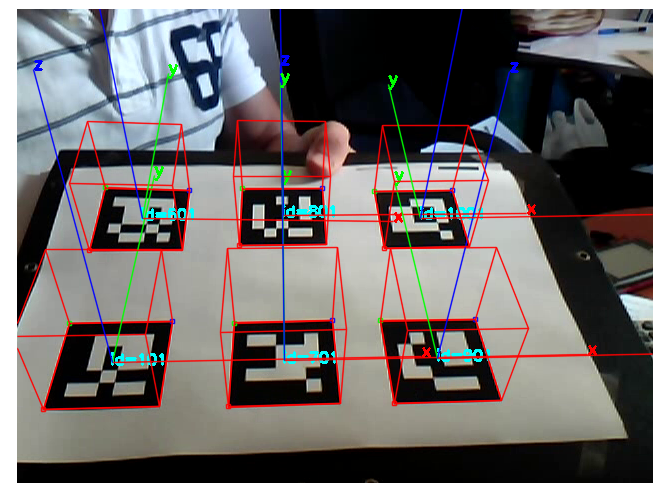
\includegraphics[scale=0.6, angle=0]{Files/Figures/aruco6.png}
    \caption[Παράδειγμα εντοπισμού marker και επαύξησης της σκηνής \cite{howmarkerswork}]{ Παράδειγμα εντοπισμού marker και επαύξησης της σκηνής \cite{howmarkerswork}}
    \label{fig:aruco5}
\end{figure}

\end{itemize}

\item Για τα έγκυρα markers, βελτιώνουμε τις γωνίες χρησιμοποιώντας subpixel παρεμβολή.


\item Τέλος, αν δίνονται οι παράμετροι της κάμερας (intrinsics), υπολογίζεται η σχετική θέση του marker ως προς την κάμερα.
\end{itemize}



Αφού εντοπιστεί η θέση του marker, ένα εικονικό μοντέλο τοποθετείται στην ίδια θέση της των συντεταγμένων της εικόνας σε σχέση με το δείκτη. Αυτό δίνει στο χρήστη την εντύπωση ότι το εικονικό αντικείμενο είναι κολλημένο πάνω στο δείκτη και η διαδικασία αυτή ονομάζεται registration. Η τελική εικόνα απεικονίζεται στην οθόνη, όπου ο χρήστης βλέπει το εικονικό αντικείμενο πάνω από την πραγματική σκηνή. Η διαδικασία πραγματοποιείται δυναμικά και αρκετά γρήγορα, ώστε να δίνεται η αίσθηση ότι της αλληλοσυσχέτισης πραγματικού και εικονικού κόσμου. Δεν είναι υπολογιστικά ακριβή διαδικασία, αλλά το marker πρέπει να αναγνωρίζεται εύκολα, π.χ οι συνθήκες φωτισμού πρέπει να είναι ευνοϊκές και δεν πρέπει να γίνεται επικάλυψη του marker, π.χ από τα χέρια του χρήστη, διότι τότε θα αποτύχει η διαδικασία της ανίχνευσης. 



\subsection{Διάταξη Πολλαπλών Markers}



Στις προηγούμενες ενότητες αναφερθήκαμε στις διαδικασίες, εκείνες, που είναι απαραίτητες για την ανίχνευση markers σε μία σκηνή με στόχο την εύρεση της σχετικής θέσης της κάμερας ως προς το marker. Ωστόσο ο εντοπισμός ενός marker μπορεί να αποτύχει για διάφορους λόγους όπως οι κακές συνθήκες φωτισμού της σκηνής, ορισμένες γρήγορες κινήσεις της κάμερας, αποκρύψεις του marker από άλλα αντικείμενα ή από τα χέρια του χρήστη κ.λ.π. 


Ένα γνωστό πρόβλημα στο tracking είναι, επίσης, το γεγονός ότι το πεδίο όρασης των καμερών (field-of-view) είναι στενό ειδικά σε φορητές συσκευές. Αν ο χρήστης μετακινήσει την κάμερα, τότε χάνεται η θέαση του marker. Έπομένως η χρήση ενός συστήματος ανίχνευσης ενός marker περιορίζει τις επιτρεπτές κινήσεις του χρήστη, καθώς η κάμερα πρέπει να βλέπει το marker συνεχώς. Για να λυθεί αυτό το πρόβλημα, ορισμένες βιβλιοθήκες επιτρέπουν τη χρήση πολλαπλών markers μαζί, τα οποία ονομάζονται πεδία markers ή markerboards. 


Ένα markerboard δεν είναι τίποτα άλλο, παρά ένας marker που αποτελείται από αρκετούς άλλους markers καθορισμένους σε μία διάταξη και παρουσιάζει δύο κύρια πλεονεκτήματα. Πρώτα απ'όλα έχει περισσότερα από ένα markers, που σημαίνει ότι είναι δυσκολότερο να χαθούν όλα την ίδια στιμή. Επίσης όσο περισσότερα markers ανιχνευθούν, τόσο περισσότερα σημεία είναι διαθέσιμα για τον υπολογισμό των εξωτερικών παραμέτρων της κάμερας. Τα συστήματα πολλαπλών markers ή αλλιώς πεδία markers (marker fields ή markerboards), συνδυάζουν την πληροφορία από όλα τα markers και επομένως παρουσιάζουν μεγαλύτερη ακρίβεια.\cite{yoon2006increasing}.



Τα συστήματα επαυξημένης πραγματικότητας καλούνται, επομένως, να βελτιώσουν την χρησιμότητα και τη ανθεκτικότητα ενός συστήματος αξιοποιώντας markersboards. Σε αυτή την ενότητα, περιγράφουμε πώς ένα σύστημα επαυξημένης πραγματικότητας μπορεί να ορίσει και να ανιχνεύσει μια διάταξη από markers.



Συγκεκριμένα, μπορούν να διαχειριστούν μερικές αποκρύψεις και να εξάγουν τη θέση ενός marker ακόμα και αν είναι αόρατο, αρκεί να γίνει η ανίχνευση άλλων markers που ανήκουν στο ίδιο πεδίο των markers. Προκειμένου να εξάγουμε τη θέση ενός μη εντοπισμένου marker, ένα σύστημα πρέπει να ξέρει τη σχετική θέση ενός marker σε σχέση με τα άλλα. Είτε η σχετική θέση των markers πρέπει να είναι προκαθορισμένη, ή το σύστημα πρέπει να επιτρέψει την ελεύθερη κατανομή των markers και να εξάγει μία διάταξη δεικτών καθώς τα ανιχνεύει. 


Προκαθορισμένα συστήματα πολλαπλών markers χρησιμοποιούνται ευρέως και υποστηρίζονται από αρκετά εργαλεία και βιβλιοθήκες. 
Για παράδειγμα, το ARToolKit \cite{artoolkit}, η ALVAR \cite{alvar} και η ArUco\cite{aruco} διαθέτουν δυνατότητες αξιοποίησης των markerboards. Η προσέγγιση είναι η ίδια με τη χρήση ενός μεγάλου marker με περισσότερα από 4 σημεία. Ουσιαστικά, ένα markerboard είναι ένα μεγάλο marker και τα markers μέσα σε αυτό είναι υπο-χαρακτηριστικά. Ένα σύστημα multi-marker μπορεί, επίσης, να χρησιμοποιήσει ένα ανεπίπεδο προκαθορισμένο marker επίσης, για παράδειγμα οι marker μπορούν να καλύπτουν τις πλευρές ενός κύβου, ορισμένοι να είναι σε ένα τοίχο κλπ.\cite{uematsu2005ar}.


\begin{figure}[H]
    \centering
    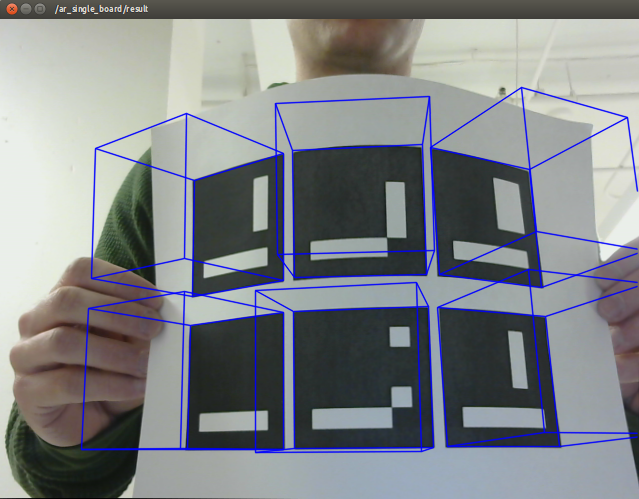
\includegraphics[scale=0.7, angle=0]{Files/Figures/markerboard_example.png}
    \caption[Παράδειγμα markerboard]{Παράδειγμα markerboard}
    \label{fig:coordinatesDiagram}
\end{figure}


Τα markers τα οποία επισυνάπτονται πάνω σε τρισδιάστατα αντικείμενα επιτρέπουν στο σύστημα να τα ανγνωρίσει από διαφορετικές οπτικές γωνίες, κάτι το οποίο είναι επιθυμητό με tangible διεπαφές.Το πρόβλημα με τις ανεπίπεδες προσεγγίσεις έχει να κάνει με το γεγονός ότι είναι δύσκολο να μετρηθεί η φυσική θέση και ο προσανατολισμός κάθε marker σε σχέση με ένα άλλο, με τη διαδικασία βαθμονόμησης να απαιτεί χρόνο και να είναι ανακριβής αν γίνει χειροκίνητα.




\section{Αναγνώριση Χειρονομιών}
%ΓΕΝΙΚΑ ΓΙΑ ΤΗΝ ΑΝΑΓΝΩΡΙΣΗ ΧΕΙΡΟΝΟΜΙΩΝ ΚΑΙ ΤΗΝ ΚΟΙΝΩΝΙΚΗ ΑΠΟΔΟΧΗ ΚΑΙ ΤΗ ΧΡΗΣΙΜΟΤΗΤΑ ΣΕ ΕΦΑΡΜΟΓΕΣ


%Από εργασία μου δερματά
Η αλληλεπίδραση του ανθρώπου με την τεχνολογία των υπολογιστών υπήρξε για πολλά χρόνια μια μηχανοκεντρική μορφή επικοινωνίας. Βασίστηκε στην ικανότητα του χρήστη να συμβιβάζεται με στρατηγικές διεπαφών που ταιριάζουν περισσότερο με την ίδια την τεχνολογία παρά με το χρήστη. Καθώς η χρήση της τεχνολογίας υπολογιστών εξαπλώνεται, οι φυσικοί και εκφραστικοί περιορισμοί των μεθόδων τους κάνει ραγδαία αντιπαραγωγικούς. Τη µεγαλύτερη ώθηση στη δηµιουργία interfaces που βασίζονται στην αναγνώριση χειρονοµίας έδωσε η ανάπτυξη εφαρµογών της περιοχής της εικονικής πραγµατικότητας, τα λεγόµενα εικονικά περιβάλλοντα. 

Οι χειρονοµίες µπορούν να ενισχύσουν τη διαδραστικότητα σε κλασσικές εφαρµογές του υπολογιστή αντικαθιστώντας το ποντίκι και ίσως σε ένα βαθµό το πληκτρολόγιο. Μπορούν επίσης να αντικαταστήσουν µοχλούς και κουµπιά σε µηχανές βασισµένες στον υπολογιστή και ακόµη µπορούν να χρησιµοποιηθούν ώς βοήθηµα για τα άτοµα µε ειδικές ανάγκες ή µε βλάβη στην όραση/ακοή ώστε να επικοινωνούν ευκολότερα µε τους συνανθρώπους τους. 


Ως αναγνώριση χειρονομιών ορίζεται η διαδικασία κατά την οποία οι χειρονομίες, οι οποίες γίνονται από τον χρήστη, αναγνωρίζονται από έναν δέκτη. Η αναγνώριση και η ερμηνεία των χειρονομιών απαιτεί από μία μηχανή την ικανότητα να μετρήσει τις δυναμικές ή στατικές παραμορφώσεις του χεριού, του βραχίονα ή ακόμα και άλλων μερών του ανθρωπίνου σώματος, τα οποία συμμετέχουν στην κίνηση.

Σε κάθε σύστημα αναγνώρισης χειρονομιών το πρώτο στάδιο είναι η συλλογή δεδομένων κατά την καταγραφή κινήσεων του χρήστη. Οι πρώτες συσκευές συλλογής δεδομένων βασιζόντουσαν στη χρήση γαντιών δεδομένων και καλωδίων, πράγμα που εμπόδιζε την φυσικότητα στην αλληλεπίδραση και περιόριζε το χρήστη και την κίνησή του μέσα στο περιβάλλον. Οι σημερινές προσεγγίσεις αξιοποιούν την χρήση βιντεοκαμερών και τεχνικών υπολογιστικής όρασης που καταγράφουν την κίνηση και με τεχνικές αναγνώρισης αναλύουν και ερμηνεύουν τις χειρονομίες.

Πολλές και ποικίλες είναι οι προσεγγίσεις των ερευνητών στο πεδίο της αναγνώρισης χειρονομιών. Αυτά που διαφέρουν σε κάθε προσέγγιση είναι ο τρόπος με τον οποίο κάθε ερευνητής κατάφερνει να συλλέξει δεδομένα και οι τεχνικές επεξεργασίας εικόνας που εφάρμόζει για να εξάγει χαρακτηριστικά. 
Οι χειρονομίες μπορούν να είναι πολύ σύνθετες, περιέχοντας ταυτόχρονες κινήσεις διάφορων σημείων, ωστόσο πρέπει η περιγραφή τους στον υπολογιστή να γίνεται με τρόπο απλό και σαφή.



%mcdonald
Έχουν προταθεί πολλές τεχνικές για την καταγραφή και την αναγνώριση των χειρονομιών [OKA02, ULHA01, CROW95]. Η ερμηνεία των χειρονομιών για το πεδίο της αλληλεπίδρασης ανθρώπου - υπολογιστή, αρχικά έγινε δυνατή χρησιμοποιώντας μετρήσεις σχετικά με την κίνηση του χεριού φορώντας ειδικά γάντια. 

Για να εφευρεθούν νέες μέθοδοι που δεν βασίζονται στην ερμηνεία επαφής με γάντια, απαιτείται η αξιοποίηση μεθόδων υπολογιστικής όρασης. Καθώς η ισχύς των επεξεργαστών συνεχίζει να αυξάνεται, οι αλγόριθμοι που κάποτε θεωρούνταν πολύπλοκοι, γίνονται διαθέσιμοι σε εφαρμογές πραγματικού χρόνου.


Το κλειδί για την απλοποίηση της δημιουργίας ενός συστήματος αναγνώρισης χειρονομιών είναι η κατασκευή ενός μοντέλου που περιγράφει ξεκάθαρα το είδος της χειρονομίας που θα ταξινομηθεί με το σχετικό σύστημα. Για να βρεθεί το μοντέλο αυτό, η εφαρμογή πρέπει να έχει οριστεί με σαφήνεια. Οι απλές απαιτήσεις χειρονομιών έχουν σαν αποτέλεσμα απλά μοντέλα χειρονομιών.

Είναι ιδιαίτερα σημαντικό, κάθε σύστημα αναγνώρισης χειρονομιών να μπορεί να διαχωρίσει την αναγνώριση μιας χειρονομίας σε σχέση με ακούσιες κινήσεις. Έχει προταθεί, για παράδειγμα, ότι το χρονικό πεδίο της ανθρώπινης χειρονομίας μπορεί να βοηθήσει στην ταξινόμηση μιας χειρονομίας έναντι μιας ακούσιας κίνησης. 



Δύο μορφές μοντελοποίησης είναι η μοντελοποίηση εμφάνισης και η μοντελοποίηση που βασίζεται σε 3Δ μοντέλο. Το πρώτο είδος μοντελοποίησης ασχολείται με την άμεση ερμηνεία της χειρονομίας από εικόνες χρησιμοποιώντας πρότυπα. Τα χαρακτηριστικά του περιεχομένου της εικόνας όπως περιγράμματα, ακμές, ορμές, ακόμα και ακροδάκτυλα μπορούν να σχηματίσουν μία βάση για την εξαγωγή παραμέτρων ως προς το μοντέλο χειρονομίας που επιλέχθηκε. Το δεύερο είδος μοντελοποίησης χρησιμοποιείται για να περιγράψει την κίνηση και τη στάση ώστε να συναχθεί η πληροφορία για τη χειρονομία. Ορισμένα σκελετικά μοντέλα περιγράφουν τις γωνίες των συνδέσμων οι οποίες μπορούν να χρησιμοποιηθούν για να συναχθεί η στάση και η ανίχνευση κίνησης.


%greek thesis
Ωστόσο δεν πρέπει να ξεχνάµε και την πολυπλοκότητα στην ανάλυση και αναγνώριση των χειρονοµιών.Τα 3D µοντέλα απαιτούν µεγάλη υπολογιστική ικανότητα απαγορευτική της χρήσης σε πραγµατικό χρόνο ενώ τα µοντέλα βασισµένα στην εµφάνιση αν και επιτρέπουν γρήγορους υπολογισµούς προσφέρονται πιο πολύ για χειρονοµίες επικοινωνίας. 




Στο κεφάλαιο αυτό παρουσιάζεται αρχικά η γενική θεωρία γύρω από το πρόβλημα της ανίχνευσης και παρακολούθησης χειρονομιών (detection and tracking of hand gestures) σε ακολουθίες εικόνων (video). Στη συνέχεια του κεφαλαίου η προσοχή επικεντρώνεται σε μια εφαρμογή του προβλήματος αυτού,
την αναγνώριση της κίνησης των ανθρώπινων χειρονομιών, που αποτελεί και το αντικείμενο της παρούσας εργασίας. Γίνεται έτσι μια εισαγωγή στη δομή του συστήματος αναγνώρισης χειρονομιών που υλοποιήθηκε, ενώ αναλυτικά το σύστημα που υλοποιήθηκε περιγράφεται στο κεφάλαιο 4.


\subsection{Εξαγωγή Blob}

Το αρχικό βήμα σε συστήματα αναγνώρισης χειρονομιών είναι η ανίχνευση των χεριών και η κατάτμηση των αντίστοιχων περιοχών της εικόνας. Η κατάτμηση αυτή είναι κρίσιμης σημασίας, διότι απομονώνει τις περιοχές ενδιαφέροντος από το παρασκήνιο της εικόνας, πριν περάσουν στην μετέπειτα παρακολούθηση τους και τα στάδια αναγνώρισης.


Στο πεδίο της όρασης υπολογιστών, η εξαγωγή blob στοχεύει στην κατηγοριοποίηση εικονοστοιχείων μιας ψηφιακής εικόνας σε ξεχωριστές ομάδες, δηλαδή στην ανίχνευση περιοχών σε μία εικόνα που διαφέρει σε ιδιότητες, όπως σε φωτεινότητα ή χρώμα σε σχέση με τις γύρω περιοχές. Άτυπα, ένα blob είναι μία περιοχή μιας εικόνας όπου κάποιες ιδιότητες είναι συνεχείς ή σχετικά συνεχείς, δηλαδή κάθε σημείο σε ένα blob μπορεί να θεωρηθεί κατά κάποιο τρόπο παρόμοιο με ένα άλλο στο ίδιο blob. Σε αυτό το πλαίσιο, ένα blob είναι ουσιαστικά ένα σχήμα που αναγνωρίζεται σε μία εικόνα και αναπαριστά ένα συγκεκριμένο αντικείμενο.


Μία εικόνα κατάτμησης είναι μία εικόνα που αναπαριστά ένα και μόνο blob, όπου τα pixels του blob είναι λευκά (255) και τα pixels του παρασκηνίου (δηλαδή όλα τα υπόλοιπα) είναι μαύρα (0). Ως ακμές των περιγραμμάτων ορίζονται οι εξωτερικές και εσωτερικές συνοριακές ακμές που διαφοροποιούν το αντικείμενο από το παρασκήνιο. 

Οι εικόνες~\ref{fig:blob1} και~\ref{fig:blob2} δείχνουν παράδειγμα μιας εικόνας κατάτμησης με τα περιγράμματά της. Η λευκή περιοχή είναι το blob που αναπαριστά το αντικείμενο, οι μαύρες περιοχές είναι το παρασκήνιο και οι κόκκινες γραμμές είναι οι γραμμές των περιγραμμάτων. Το αντικείμενο στο παράδειγμα έχει μία "τρύπα" μέσα του και επομένως έχει και μία εσωτερική ακμή περιγράμματος πέρα από το εξωτερικό περίγραμμα. 



\begin{figure}[H]
    \centering
    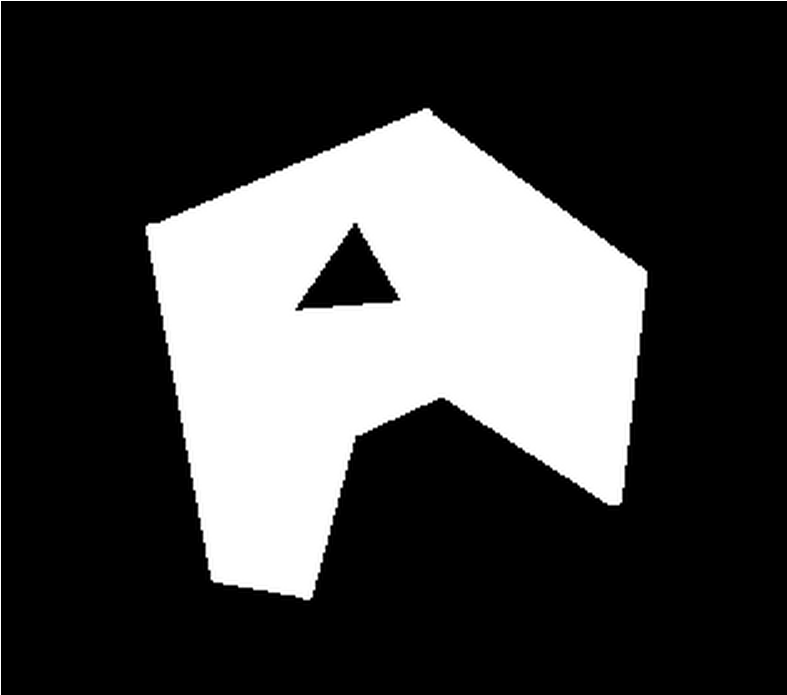
\includegraphics[scale=0.6, angle=0]{Files/Figures/blob1.png}
    \caption[Εικόνα κατάτμησης - Blob]{Εικόνα κατάτμησης - Blob}
    \label{fig:blob1}
\end{figure}



\begin{figure}[H]
    \centering
    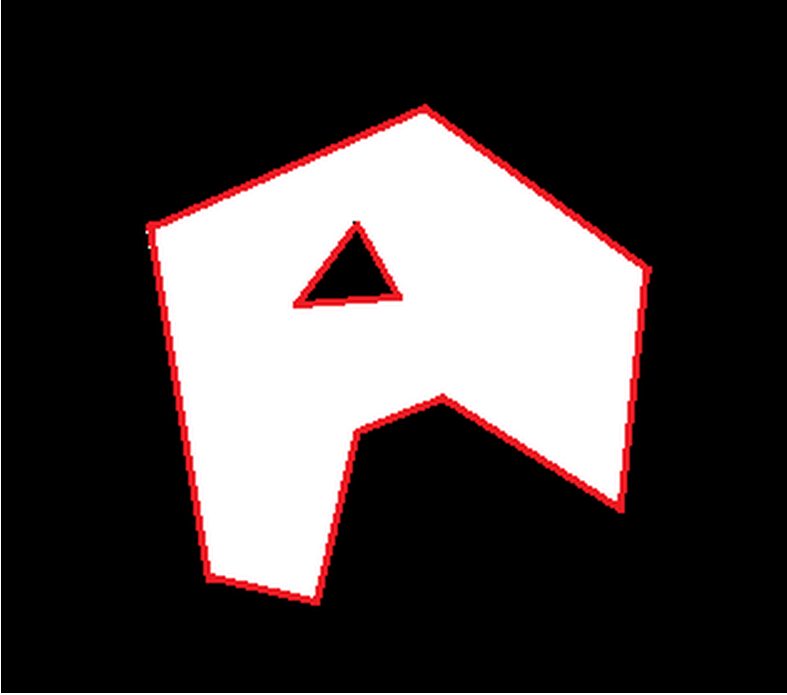
\includegraphics[scale=0.6, angle=0]{Files/Figures/blob2.png}
    \caption[Ακμές περιγραμμάτων]{Ακμές περιγραμμάτων}
    \label{fig:blob2}
\end{figure}



Μερικές προσεγγίσεις ανιχνεύουν τα χέρια, σε επίπεδο εικόνας blob σε κάθε καρέ και χρονικά αντιστοιχούν τα blob στις αντίστοιχες κοντινές περιοχές σε όλα τα frames. Οι προσεγγίσεις που βασίζονται στα blobs είναι σε θέση να διατηρήσουν την παρακολούθηση του χεριού, ακόμη και όταν υπάρχουν μεγάλες χρονικά διαστήματα από καρέ σε καρέ.



\subsection{Αναγνώριση Χειρονομίας Τσιμπήματος}
%ANALYΣΕ ΤΟ PINCH, ΠΩΣ ΓΙΝΕΤΑΙ, ΓΙΑΤΙ ΕΙΝΑΙ ΕΥΚΟΛΟ,ΠΟΥ ΧΡΗΣΙΜΟΠΟΙΕΙΤΑΙ, ΠΩΣ ΑΝΙΧΝΕΥΕΤΑΙ(WILSON,ETC)

%hoggan
Οι χειρονομίες χρησιμοποιούνται ως μέσο αλληλεπίδρασης σε πολλά διαφορετικά είδη συσκευών και εφαρμογών. Μία από τις πιο γνωστές χειρονομίες είναι αυτή της χειρονομίας του "τσιμπήματος", που περιλαμβάνει την διαστολή ή συστολή της έκτασης των δακτύλων \cite{hoggan2013multi}.


Η χειρονομία "τσιμπήματος" θεωρείται μία από τις κοινότερες χειρονομίες για αλληλεπίδραση με ψηφιακές διεπαφές. 
Έχει χρησιμοποιηθεί για διαφορετικούς σκοπούς ανάλογα με το πεδίο των εφαρμογών, όπως για παράδειγμα ως μεταφορική χειρονομία για μεγέθυνση, κλιμάκωση ή επιλογή. Μοιάζει με κίνηση αρπαγής (grabbing) ή επιλογής και δείχνει ένα φυσικό σήμα επιλογής ή μετακίνησης ενός αντικειμένου σε ένα διαδραστικό σύστημα. 

Κατά τη διάρκεια της αλληλεπίδρασης με πραγματικά αντικείμενα, χρησιμοποιείται για το άρπαγμα μικρών κομματιών ή μαλακών αντικειμένων όπως υφάσματα. Μοιάζει με μία κίνηση αρπαγής ή επιλογής και προσφέρει ένα φυσικό σήμα για την επιλογή ή τη μετακίνηση ενός αντικειμένου σε ένα διαδραστικό σύστημα.



Η χειρονομία αυτή μπορεί να εντοπιστεί σχετικά εύκολα, διότι δεν υπάρχει αμφιβολία αν ο αντίχειρας αγγίζει τον δείκτη ή όχι. Μάλιστα, λόγω της φύσης των δακτύλων δείκτη και αντίχειρα, η χειρονομία τσιμπήματος είναι ακριβής και υψηλών επιδόσεων.



Αν και οι προσεγγίσεις που βασίζονται σε 3Δ μοντέλα μπορούν να καταγράψουν το μεγαλύτερο σύνολο των χειρονομιών στο πεδίο της αλληλεπίδρασης ανθρώπου-υπολογιστή, οι εφαρμογές που χρησιμοποιούν αυτές τις μεθόδους λειτουργούν σπάνια σε πραγματικό χρόνο. Οι περισσότερες προσεγγίσεις αξιοποιούν μοντέλα που βασίζονται στην εμφάνιση (appearance-based models) \cite{Wang2011}.

Για τους σκοπούς της συγκεκριμένης εργασίας και με βάση τις πιο κοινά χρησιμοποιημένες χειρονομίες όπως περιγράφονται στο \cite{Piumsomboon2013}, το "τσίμπημα" είναι μία καίρια χειρονομία για την υλοποίηση αλληλεπιδράσεων μέσα στο χώρο της επαυξημένης πραγματικότητας.

Η χειρονομία αυτή είναι ιδανική για την αλληλεπίδραση μέσω χειρονομιών, καθώς είναι εύκολο να πραγματοποιηθεί και να εντοπιστεί και σε αντίθεση με άλλες χειρονομίες δεν απαιτεί χρονικό όριο, ενώ μπορεί να ανιχνευθεί εύκολα, διότι κατά τη διεξαγωγή της, αρκεί να εντοπιστεί η "τρύπα" που σημιουργείται στο χέρι, μόλις ο δείκτης αγγίξει τον αντίχειρα με χρήση τεχνικών υπολογιστικής όρασης.



\section{Σχετικές Ερευνητικές Εργασίες}
%ΑΝΑΦΕΡΕ ΠΑΡΟΜΟΙΕΣ ΕΡΓΑΣΙΕΣ ΓΙΑ GESTURE INTERACTION, AR TABLETOP GAMING
%ΠΕΣ ΣΙΓΟΥΡΑ ΓΙΑ ΠΑΡΟΜΟΙΑ ΣΚΑΚΙΑ ΣΤΟ ΤΕΛΟΣ
%ΨΑΧΝΟΝΤΑΣ ΣΕ PAPERS ΑΝΑΦΕΡΕ ΠΑΡΟΜΟΙΕΣ ΕΡΓΑΣΙΕΣ ΝΑ ΕΧΟΥΝ ΣΧΕΣΗ ΜΕ GESTURE RECOGNITION FOR AR, VIRTUAL OBJECT MANIPULATION, AR TABLETOP GAMES


Σε προηγούμενες ερευνητικές εργασίες, παρουσιάστηκαν διαφορετικές προσεγγίσεις για την κατανόηση των δυνατοτήτων που προσφέρουν οι χειρονομίες στην αλληλεπίδραση με εικονικά αντικείμενα σε ένα περιβάλλον επαυξημένης πραγματικότητας. Επιπλέον, σε βιβλιογραφικές αναφορές μπορούμε να εντοπίσουμε τις δυνατότητες της επαυξημένης πραγματικότητας στον χώρο της ψυχαγωγίας και συγκεκριμένα των βιντεοπαιχνιδιών, τις βασικές έννοιες της αλληλεπίδρασης μεσω χειρονομιών και της ρεαλιστικής απεικόνισης εικονικών αντικειμένων.



%AR TABLETOP GAMING

Ένα παιχνίδι επαυξημένης πραγματικότητας με την ονομασία Facade, επεκτάθηκε σε μία επαυξημένη έκδοση με χρηση ενός HMD. Το παιχνίδι αυτό \cite{Dow2007} διέφερε πολύ από τις παραδοσιακές ιδέες για βιντεοπαιχνίδια επαυξημένης πραγματικότητας που είχαν υλοποιηθεί προηγουμένως. Πρόκειται για ένα περίπλοκο παιχνίδι ρόλων που μοιάζει με διαδραστικό θέατρο. Το συγκεκριμένο βιντεοπαιχνίδι χρησιμοποιεί χειρονομίες και φωνητικές εντολές ως κύριες μορφές αλληλεπίδρασης. Τα αντικείμενα τα οποία μπορούσαν να χειριστούν τόσο οι εικονικοί, όσο και οι πραγματικοί χρήστες παρουσιάζονταν ως αντικείμενα επαυξημένης πραγματικότητας στον παίκτη μέσω του HMD.


%playstation app with board and monitor for AR
Το βιντεοπαιχνίδι Eye of Judgement της πλατφόρμας Sony PS3 είναι ένα βιντεοπαιχνίδι επαυξημένης πραγματικότητας σε τρίτο πρόσωπο, που περιλαμβάνει μία ψηφιακή βιντεοκάμερα η οποία καταγράφει το ταμπλό του παιχνιδιού και απεικονίζει μία επαυξημένη του έκδοση στην τηλεόραση. Αυτός ο τύπος παιχνιδιού απαιτεί από τους χρήστες να επικεντρώνουν την προσοχή τους τόσο στο πραγματικό ταμπλό, όσο και στην έκδοση που παρουσιάζεται στην οθόνη. Μόλις οι κάρτες του παιχνιδιού τοποθετηθούν πάνω στο ταμπλό, δρουν ως καθοδηγητικοί δείκτες(markers) για τον εντοπισμό τεράτων επαυξημένης πραγματικότητας και τα κομμάτια του παιχνιδιού απεικονίζονται επάνω τους. Η μηχανή παιχνιδιών αναλαμβάνει τα τρισδιάστατα γραφικά των καρτών μόλις εντοπιστούν. Το παιχνιδί αυτό, ήταν ένα από τα πρώτα εμπορικά βιντεοπαιχνίδια επαυξημένης πραγματικότητας που κυκλοφόρησαν στην αγορά που επέτρεπε τη χρήση καθογητητικών δεικτών (fiducial markers) \cite{Thomas2010}.



\begin{figure}[H]
    \centering
    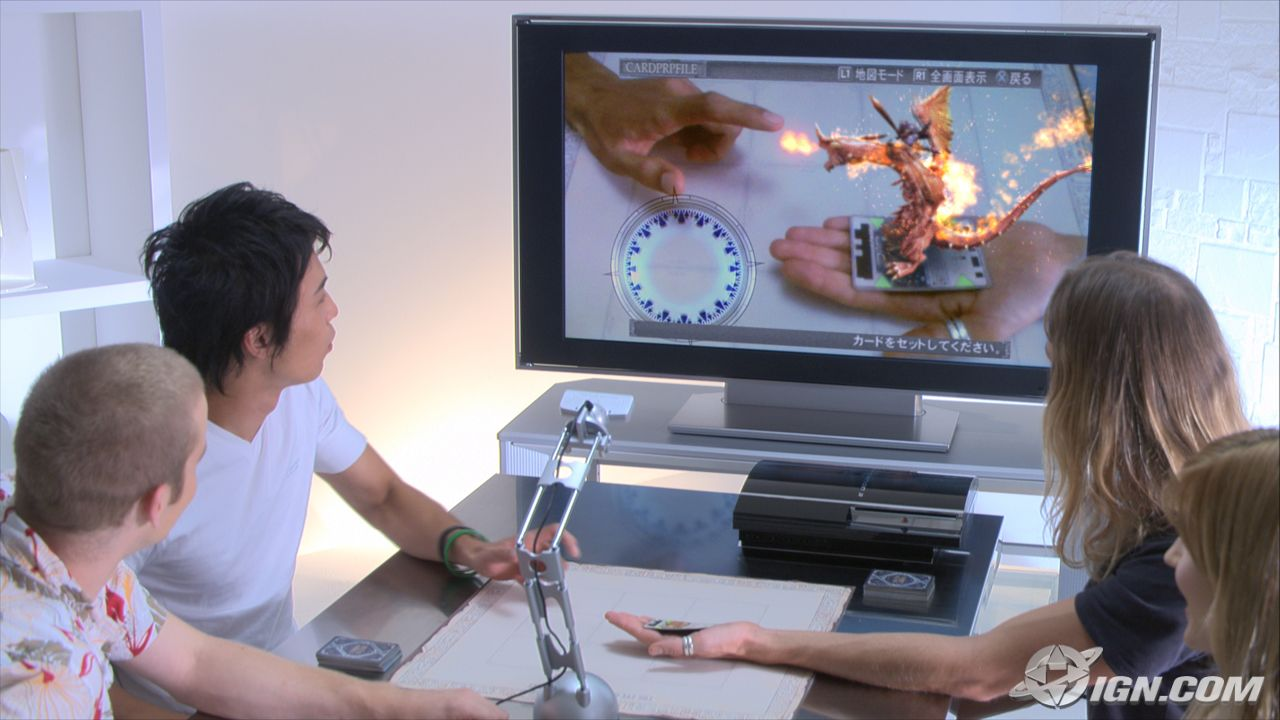
\includegraphics[scale=0.2, angle=0]{Files/Figures/eyejudgment.jpg}
    \caption[Eye of Judgement Game]{Eye of Judgement Game}
    \label{fig:ps3game}
\end{figure}



%GESTURES IN AR

Το 2006 ο A. Wilson παρουσίασε μία τεχνική όρασης υπολογιστών που επιτρέπει την ανίχνευση της επαφής ενός δείκτη με τον αντίχειρα ενός χρήστη (χειρονομία "τσιμπήματος" υπό συνθήκες κοντινών αποστάσεων \cite{Wilson2006}. Η τεχνική αυτή αποφέυγει πολύπλοκους και εύθραυστους αλγορίθμους ανίχνευσης χεριών εντοπίζοντας απλά την "τρύπα" που δημιοργείται όταν ο δείκτης ακουμπήσει τον αντίχειρα. Η εργασία αυτή χρησιμοποιήθηκε από μεγάλο εύρος επιστημονικών εργασιών για το χειρισμό εικονικών αντικειμένων και όχι μόνο.



Για παράδειγμα, με βάση την παραπάνω τεχνική, το 2009, ο Hilliges και συνάδελφοί του χρησιμοποίησαν μία κάμερα βάθους για τον εντοπισμό χειρονομιών "τσιμπήματος" πάνω από ένα τραπέζι \cite{Wilson2}. Ενώ συνήθως ο χειρισμός των αντικειμένων που απεικονίζονταν στην επιφάνεια ενός ειδικού διαδραστικού τραπεζιού γινόταν σε 2 διαστάσεις, η εργασία αυτή κατάφερε να σχεδιάσει μια τεχνική που επιτρέπει στα εικονικά αντικείμενα να επιλεγούν και να μετακινηθούν και στις 3 διαστάσεις. Οι χρήστες είχαν τη δυνατότητα να σηκώσουν τα αντικείμενα και να τα αφήσουν σε κάποια άλλη θέση.




Σε μία άλλη εργασία \cite{Lee2008}, περιγράφεται ένα σύστημα που βασίζεται σε τεχνικές όρασης υπολογιστών για τον εντοπισμό των χεριών στο 3D χώρο με στόχο τη δημιουργίας μιας διεπαφής επαυξημένης πραγματικότητας.  Υλοποιήθηκε μία φυσική μέθοδος αλληλεπίδρασης με τα χέρια που βασίζεται στην 3D όραση και αποτελείται από 4 βήματα που περιλαμβάνουν την κατάτμηση με βάση το χρώμα του δέρματος, την εύρεση χαρακτηριστικών σημείων, τον υπολογισμό της κατεύθυνσης του χεριού και την ανίχνευση συγκρούσεων με βάση μία μικρή ακτίνα από το δάκτυλο του χρήστη για την αλληλεπίδραση ανάμεσα στο χέρι του χρήστη και τα εικονικά αντικείμενα. Παρά το γεγονός ότι οι χρήστες μπορούν να χρησιμοποιήσουν το σύστημα της διεπαφής για αλληλεπίδραση σε περιβάλλοντα επαυξημένης πραγματικότητας, η χρήση ενός και μόνο δακτύλου (του δείκτη) για την αλληλεπίδραση φάνηκε επιρρεπής σε λάθη διότι το δάκτυλο είναι πολύ λεπτό για να υπολογιστεί η στερεοσκοπική διαφορά. Επίσης οι συγγραφείς πιστεύουν ότι χρειάζεται περισσότερη ακρίβεια, φυσικότητα και ταχύτητα.



Το 2013 ο Bai κ.α παρουσίασαν μία μέθοδο αλληλεπίδρασης μέσω χειρονομιών για εφαρμογές επαυξημένης πραγματικότητας σε φορητές συσκευές \cite{Bai2013}. Για να συμβεί αυτό, χρειάστηκε η σύνδεση ενός αισθητήρα χρώματος - βάθους με ένα tablet.
Συνδυάζοντας την πληροφορία βάθους με τις χειρονομίες, η αλληλεπίδραση μπορεί να επεκταθεί σε ολόκληρο το 3D χώρο. Στο σύστημα που αναπτύχθηκε, γίνεται ανάκτηση του 3D σκελετού του χεριού από τα frames χρώματος και βάθους και τα αποτελέσματα αντιστοιχίζονται στο χειρισμό των εικονικών αντικειμένων στην επαυξημένη σκηνή. Η μέθοδος αυτή επιτρέπει τον έλεγχο των εικονικών αντικειμένων στον 3D χώρο με τη χρήση γυμνών χεριών και την εκτέλεση διεργασιών όπως η μετακίνηση, η περιστροφή και η μεγέθυνση. 

\begin{figure}[H]
    \centering
    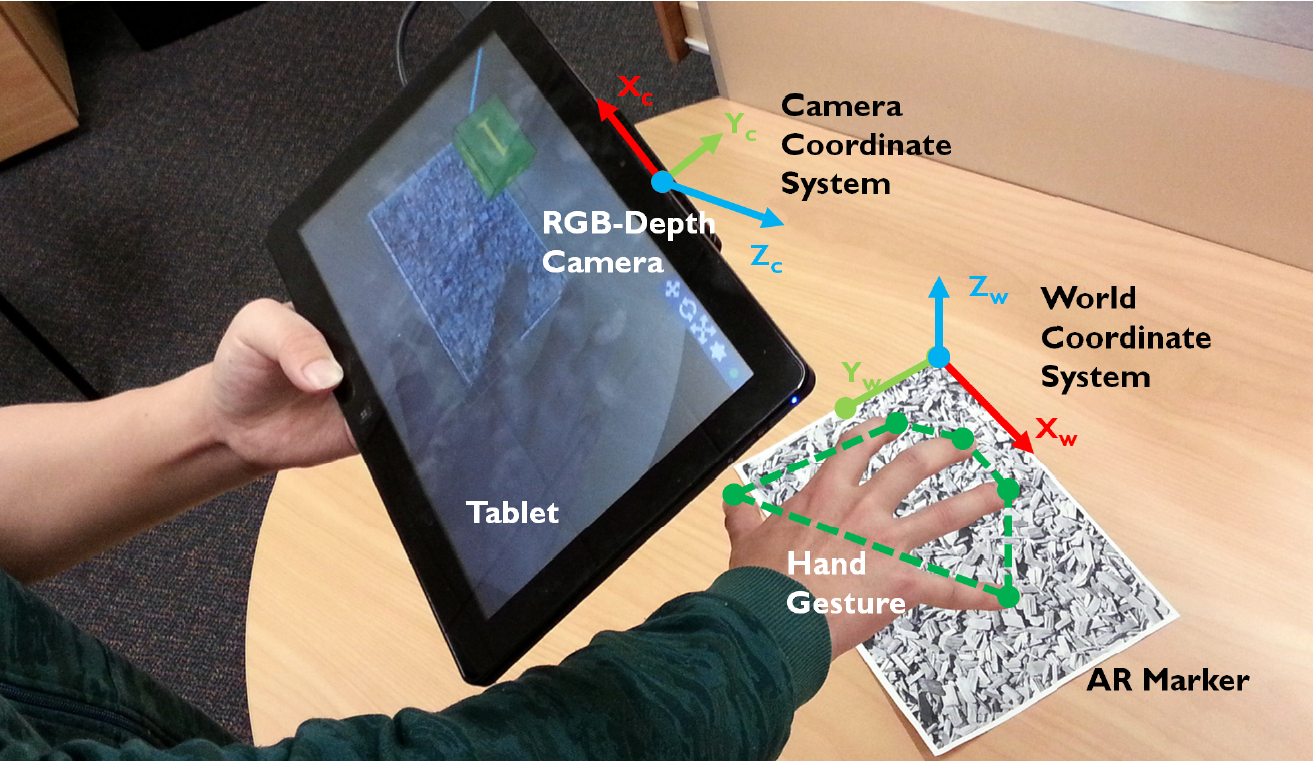
\includegraphics[scale=0.5, angle=0]{Files/Figures/BaiApp.png}
    \caption[Το σύστημα που αναπτύχθηκε για φορητές συσκευές]{Το σύστημα που αναπτύχθηκε για φορητές συσκευές}
    \label{fig:ps3game}
\end{figure}



%google glass manipulation project
Η αλληλεπίδραση με εικονικά αντικείμενα μέσω χειρονομιών για εφαρμογές επαυξημένης πραγματικότητας επιχειρήθηκε και για συσκευές όπως το Google Glass \cite{Bai2014} . Όπως επισημαίνουν οι συγγραφείς, ο εντοπισμός του χειριού είναι ιδιαίτερα δύσκολος, αν κάποιος θέλει να δημιουργήσει ένα ολοκληρωμένο 3D σκελετικό μοντέλο, ενώ το Google Glass δεν έχει τους κατάλληλους αισθητήρες και την υπολογιστική δύναμη για να πραγματοποιήσει κάτι τέτοιο σε πραγματικό χρόνο.
Για το λόγο αυτό, πραγματοποίησαν τον εντοπισμό του χεριού σε έναν υπολογιστή και επέλεξαν να στείλουν το αποτέλεσμα στο Glass για την απεικόνιση και την αλληλεπίδραση. Αυτό επιτρέπει την ολοκληρωμένη 3D αλληλεπίδραση σε πραγματικό χρόνο. Συγκεκριμένα σύνδεσαν έναν αισθητήρα χρώματος - βάθους με έναν υπολογιστή για την παραγωγή 3D μοντέλα πραγματικού χρόνου και των δυο χεριών στο χώρο από κάτω από τον αισθητήρα, ενώ χρησιμοποιήσαν μία εικόνα σαν ως σημείο αναφοράς για τις συντεταγμένες. Έτσι συνδύασαν το σύστημα συντεταγμένων του αισθητήρα χρώματος - βάθους και του Google Glass στην ίδια σκηνή, με αποτέλεσμα να μοιράζονται το ίδιο σύστημα συντεταγμένων κόσμου με βάση το marker εικόνα. Το 3Δ μοντέλο χεριού που εντοπίζεται από τον υπολογιστή μπορεί να μεταδοθεί στο Glass μέσω ενός ασύρματου δικτύου σε πραγματικό χρόνο. Έτσι γίνεται δυνατή η χρήση του χεριού ως 3D είσοδος στο σύστημα. Πέρα από τον εντοπισμό της θέσης του χεριού και του σχήματος του, το λογισμικό που υλοποιήθηκε επιτρέπει την αναγνώριση απλών χειρονομιών όπως είναι η χειρονομία "τσιμπήματος". 


\begin{figure}[H]
    \centering
    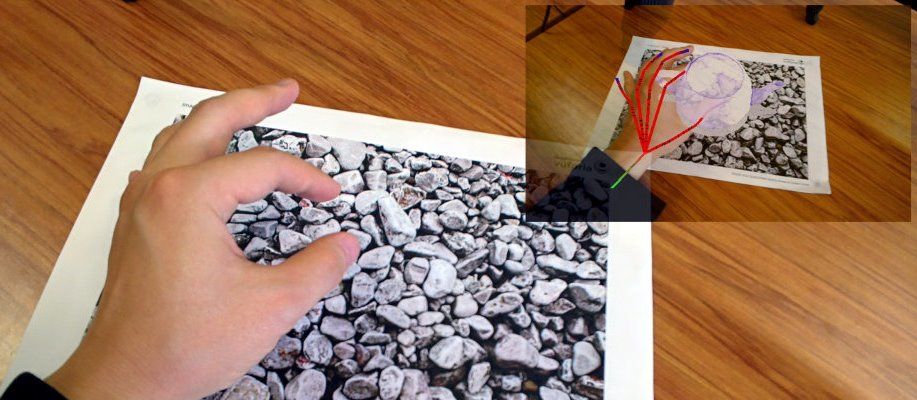
\includegraphics[scale=0.3, angle=0]{Files/Figures/GestureBannerFinal1.png}
    \caption[Google Glass interaction]{Google Glass interaction}
    \label{fig:ps3game}
\end{figure}






%SKAKIA APO TUGRAZ
Στη βιβλιογραφία εντοπίζονται 2 επιστημονικές εργασίες, όπου παρουσιάζονται υλοποιήσεις σκακιών επαυξημένης πραγματικότητας. Στην πρώτη εργασία \cite{Reitmayr2001}, χρησιμοποιήθηκε ένα 
φορητό βοήθημα σαν στυλό, πάνω στο οποίο τοποθετήθηκε ένας κύβος, οι πλευρές του οποίου είχαν ένα marker. Με αυτό τον τρόπο γινόταν δυνατή η αλληλεπίδραση με ψηφιακά πιόνια σκακιού Όπως παραδέχονται και οι συγγραφείς, ο εντοπισμός των markers πάνω στο στυλό δεν ήταν ιδιαίτερα ακριβής, ενώ παράλληλα ήταν αργός για να επιτευχθεί απρόσκοπτη και φυσική χρήση.

Την ίδια χρονιά, οι Dorfmuller-Ulhaas και Schmalstieg δημιούργησαν ένα σύστημα οπτικής ανίχνευσης δακτύλων, με απώτερο σκοπό την αφαίρεση των ενοχλητικών καλωδίων κατά τη διάρκεια της αλληλεπίδρασης με τα εικονικά αντικείμενα \cite{Dorfmuller-Ulhaas2001}. Μάλιστα, η τεχνολογίας που ανέπτυξαν, παρουσιάστηκε μέσα από μία επαυξημένη έκδοση ενός παιχνιδιού σκακιού. Οι συγγραφείς αξιοποίησαν τεχνικές εντοπισμού των δακτύλων για την αλληλεπίδραση μέσω χειρονομιών με εικονικά πιόνια.  Πιο συγκεκριμένα χρησιμοποίησαν χειρονομίες αρπαγής και αποδέσμευσης (grab and release gestures), καθώς και τεχνικές επεξεργασίας εικόνας για τον εντοπισμό των χειρονομιών, μέσω μιας κάμερας. Ο ανιχνευτής δακτύλων που υλοποιείται αξιοποιεί ένα 3D μοντέλο χεριού, το οποίο μπορεί να καθορίσει αρκετές πληροφορίες για τον απρόσκοπτο εντοπισμό της θέσης, του προσανατολισμού και της πόζας του δείκτη των χρηστών. Ωστόσο, η προσέγγιση αυτή απαιτεί τη χρήση ενός γαντιού με σφαίρες αντανάκλασης που τοποθετούνται ακριβώς πάνω από τους συνδέσμους των δακτύλων, κάτι το οποίο μπορεί να ενοχλεί τους χρήστες και σίγουρα δεν ενθαρρύνει έναν φυσικό τρόπο αλληλεπίδρασης με το εικονικό περιεχόμενο. 



%pes kai gia skaki tis meta
Το 2014, η εταιρία Meta δημιούργησε μια σειρά ειδικών γυαλιών επαυξημένης πραγματικότητας με την ονομασία Meta One και Meta Pro, που συνδυάζουν τον πραγματικό κόσμο με ολογραφικές εικόνες. Για την προώθηση των συγκεκριμένων προϊόντων, δημιούργησαν ένα διαφημιστικό βίντεο \cite{metaglasses}, όπου παρουσιάζονται δύο χρήστες να παίζουν σκάκι με εικονικά πιόνια και σκακιέρα, χρησιμοποιώντας τα γυαλιά και τα χέρια τους, χωρίς κάποιο άλλο βοήθημα, όπως γάντια, markers κ.λπ. Παρά το γεγονός ότι το βίντεο αυτό παρουσιάζει μία ιδανική προσέγγιση για ένα σκάκι επαυξημένης πραγματικότητας, δεν αποτελεί πραγματικά υλοποιημένη εφαρμογή, ωστόσο αποτέλεσε πηγή έμπνευσης για τη συγκεκριμένη εργασία.




%epilogos
Η ποικιλομορφία συσκευών, εργαλείων και εφαρμογών επαυξημένης πραγματικότητας είναι εντυπωσιακή. Γενικά, η τεχνολογία της επαυξημένης πραγματικότητας είναι μια μέθοδος απεικόνισης που μπορεί να χρησιμοποιηθεί σε πολλές εφαρμογές, ενώ παράλληλα επιτρέπει φυσικές αλληλεπιδράσεις και είναι ένα καλό εργαλείο ανάπτυξης διαδραστικών βιντεοπαιχνιδιών που μπορεί να ενισχύσει την εμπειρία που βιώνουν οι χρήστες. Σε αυτή την εργασία, στοχεύουμε στη δημιουργία μιας μεθόδου αναγνώρισης χειρονομιών τσιμπήματος που μπορεί να χρησιμοποιηθεί για το διαδραστικό, απλό και γρήγορο χειρισμό εικονικών αντικειμένων σε περιβάλλοντα επαυξημένης πραγματικότητας. Οι αλγόριθμοι που αναπτύσσονται, εξετάζονται και αξιολογούνται υλοποιώντας ένα βιντεοπαιχνίδι επαυξημένης πραγματικότητας του γνωστού επιτραπέζιου παιχνιδιού, του σκακιού.




 
